\documentclass{phyasgn}\usepackage{nag}
\phyasgn{classname=挑战杯五四青年科学项目}
\usepackage{siunitx}
\usepackage{subfig}
%\ctexset{punct=kaiming}
\setCJKmainfont[ItalicFont=FZKTK.TTF,BoldFont=FZXBSK.TTF]{FZSSK.TTF}
\setCJKsansfont[BoldFont=FZHTK.TTF]{FZXH1K.TTF}
\setCJKmonofont[ItalicFont=FZKTK.TTF]{FZFSK.TTF}
\newCJKfontfamily\FZSS{FZSSK.TTF}
\newCJKfontfamily\FZKT{FZKTK.TTF}
\newCJKfontfamily\FZFS{FZFSK.TTF}
\newCJKfontfamily\FZHT{FZHTK.TTF}
\setmainfont{TeX Gyre Termes}
\setsansfont{TeX Gyre Heros}[Scale=MatchLowercase]
\setmonofont{Ubuntu Mono}%[Scale=MatchLowercase]
\newfontfamily\lm{Latin Modern Roman}
\usepackage{unicode-math}
\setmathfont{TeX Gyre Termes Math}
\newcommand\keywords[1]{\textbf{关键词}: #1}
\newcommand{\enabstractname}{Abstract}
\newenvironment{enabstract}{%
  \par\small
  \noindent\mbox{}\hfill{\bfseries \enabstractname}\hfill\mbox{}\par
  \vskip 1ex}{\par\vskip 1ex}
\newcommand\pkg[1]{\textsf{#1}}
\newenvironment{csop}{\vskip\topsep\noindent\hspace{2em}\ttfamily\small\ignorespaces}{\vskip\topsep\par}
\usepackage{float}
\usepackage{booktabs,metalogo,siunitx,marginnote,manfnt,url}
\usepackage[unicode]{hyperref}
\hypersetup{pdfstartview=XYZ,hidelinks,pdfcreator=XeTeX Output,pdfauthor=xxx,
pdftitle=抗议、镇压与宣传反制:来自哥伦比亚的证据}
\urlstyle{same} 
\usepackage{geometry,fancyhdr}
\geometry{left=3cm,right=3cm,marginparwidth=4em}
\fancyhead[L]
{\begin{tabular}[b]{@{}l@{}}
  \hyperref{https://www.pku.edu.cn/}{}{}{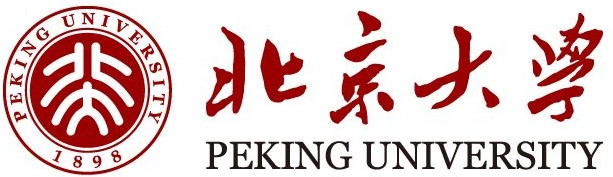
\includegraphics[height=2.12em]{pkulogo.jpg}}
\end{tabular}}
\fancyhead[C]
{
  \large 
  抗议、镇压与宣传反制:来自哥伦比亚的证据
}

\usepackage{shortvrb,fancyvrb}
\MakeShortVerb|
\fvset{xleftmargin=2em,fontsize=\small}
\makeatletter
\ifx\l@nohyphenation\undefined
  \newlanguage\l@nohyphenation
\fi
\DeclareRobustCommand\meta[1]{%
  \ensuremath\langle
  \ifmmode \expandafter \nfss@text \fi
  {%
    \rmfamily\itshape
    \edef\meta@hyphen@restore
    {\hyphenchar\the\font\the\hyphenchar\font}%
  \hyphenchar\font\m@ne
  \language\l@nohyphenation
  #1\/%
  \meta@hyphen@restore
  }\ensuremath\rangle
}
\makeatother

\def\phyasgn{\pkg{phyasgn}}
\def\version{0.2 $\upbeta$}

\title{
  {抗议、镇压与宣传反制:来自哥伦比亚的证据}\\[-8pt]
    {\Large ——附录部分}
}
\author{小组成员:张维翰\thanks{200001694
8@stu.pku.edu.cn,政府管理学院,公共管理类},邓晨钰\thanks{dengcheny
u11@126.com,外国语学院,西班牙语专业},范一苇\thanks{fyw233@outlook.com,外国语学院,西班牙语专业},姜雨玥\thanks{2100018504@stu.pku.edu.cn,外国语学院,西班牙语专业},邱文治\thanks{own@pku.edu.cn,历史学系,外国语言与外国历史专业},吴熙楠\thanks{xinanwu@pku.edu.cn,物理学院,物理专业}}
\date{\today}
\begin{document}
\maketitle
\tableofcontents
\clearpage
\appendix
\section{数据检验}
\begin{figure}[!h]
                    	\centering
                    	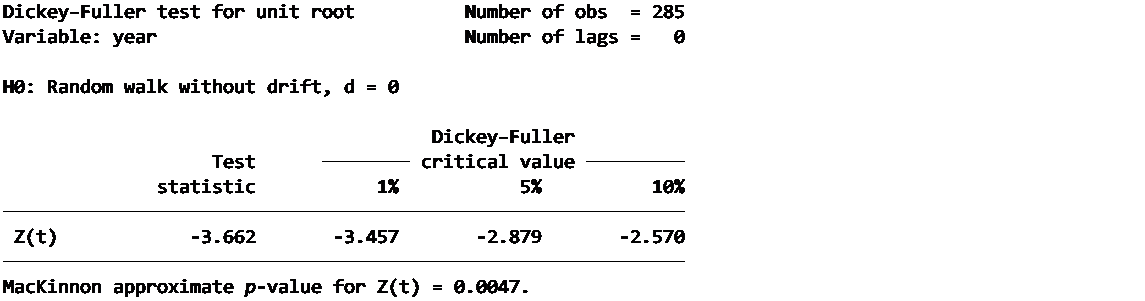
\includegraphics[width=1.0\linewidth]{pic/18.png}
                    	\caption{平稳性检验结果}
                    	\end{figure}
\begin{figure}[!h]
                    	\centering
                    	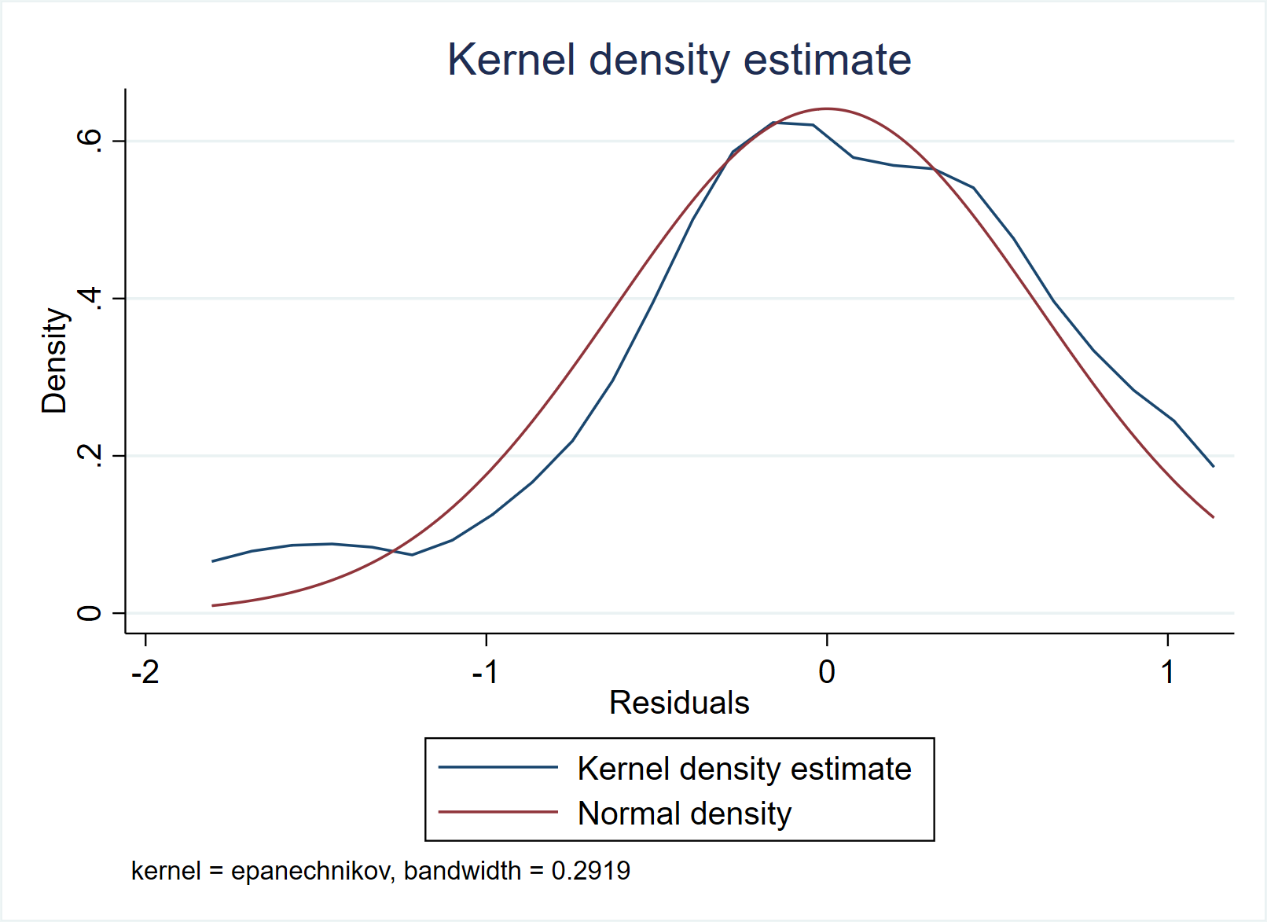
\includegraphics[width=1.0\linewidth]{pic/19.png}
                    	\caption{残差正态性检验结果(1)}
                    	\end{figure}
\begin{figure}[!h]
                    	\centering
                    	
\includegraphics[width=1.0\linewidth]{pic/20.png}
                    	\caption{残差正态性检验结果(2)}
                    	\end{figure}
\begin{figure}[!h]
                    	\centering
                    	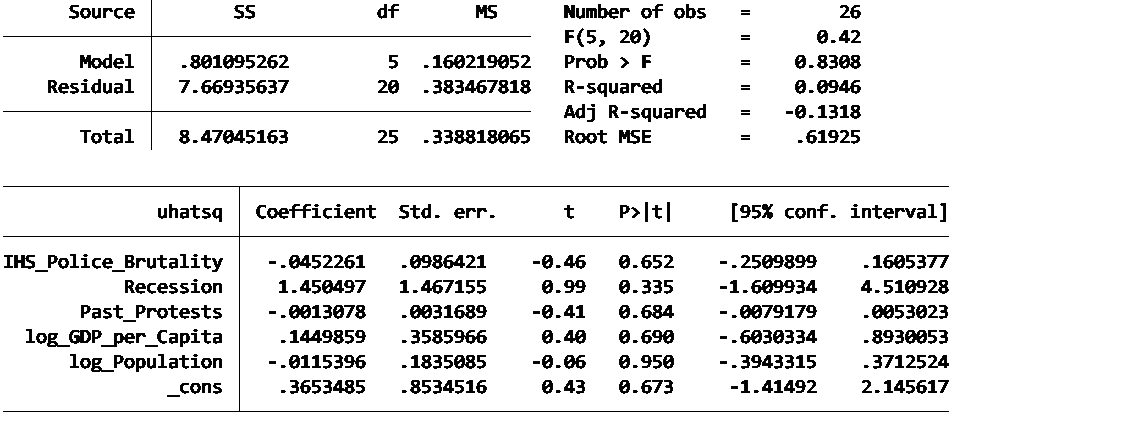
\includegraphics[width=1.0\linewidth]{pic/21.png}
                    	\caption{异方差检验结果}
                    	\end{figure}
\begin{figure}[!h]
                    	\centering
                    	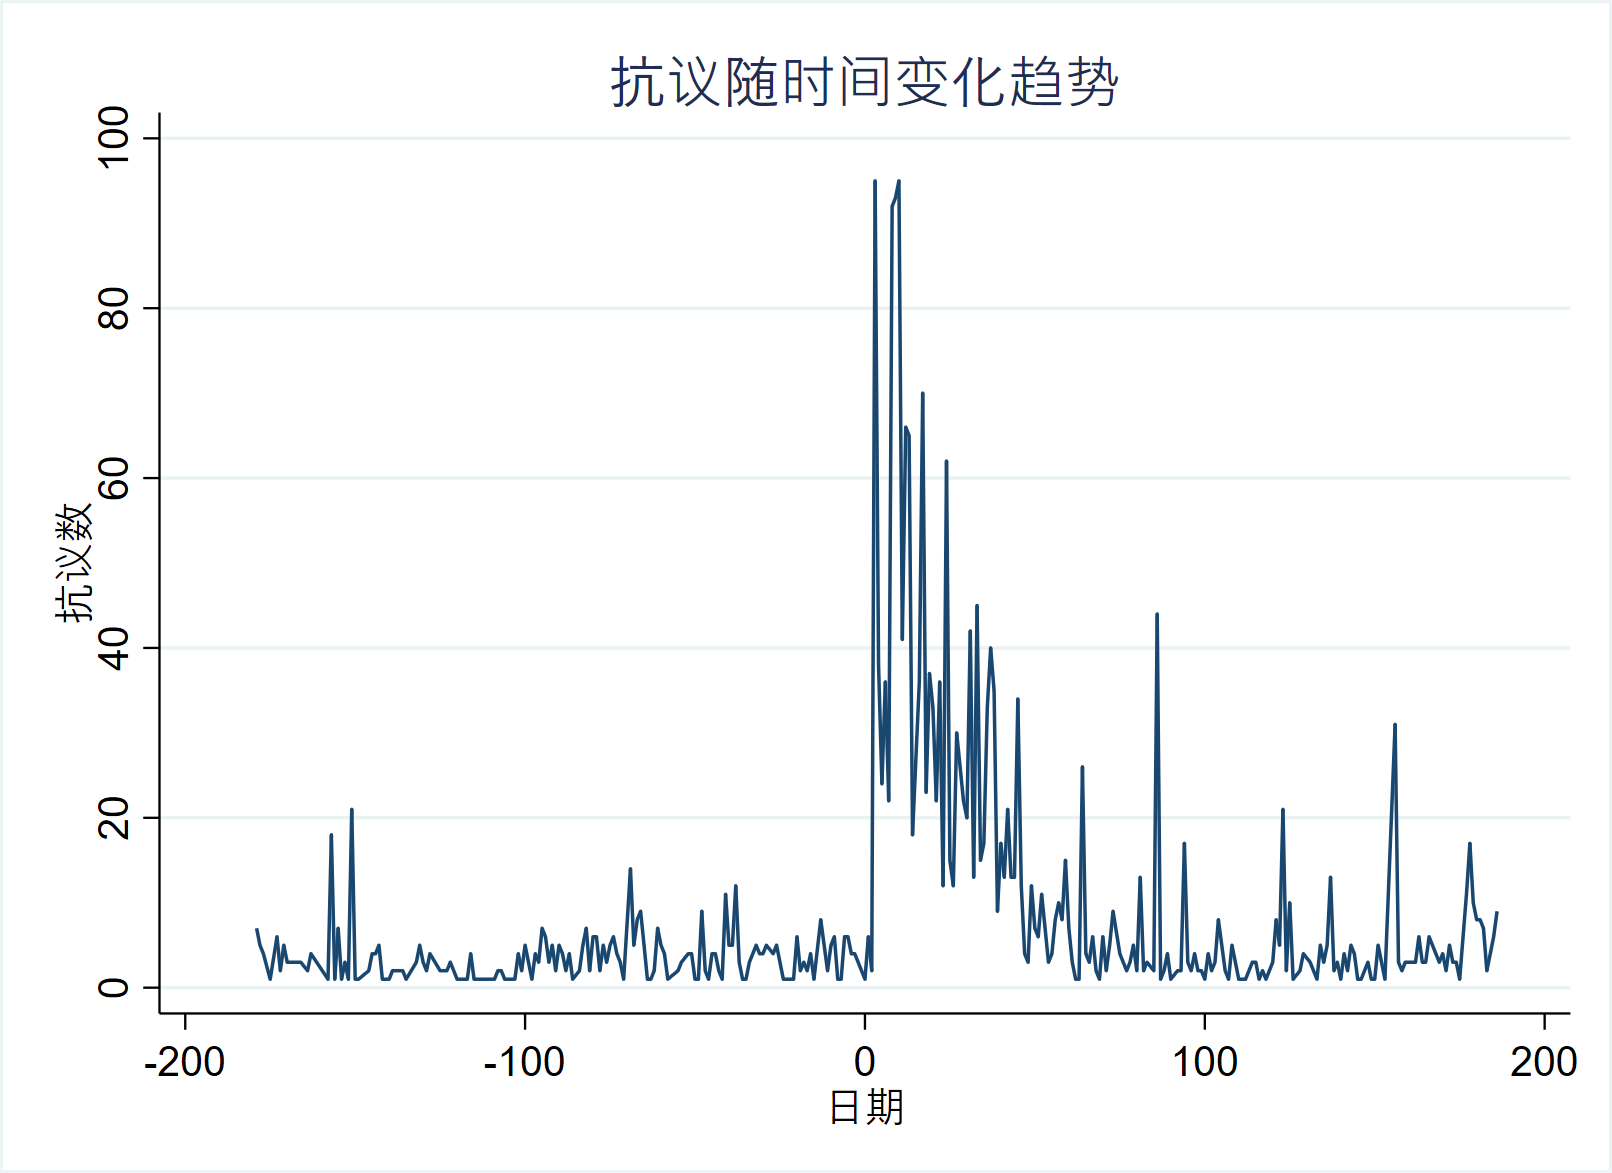
\includegraphics[width=1.0\linewidth]{pic/22.png}
                    	\caption{抗议随时间变化趋势}
                    	\end{figure}
\begin{figure}[!h]
                    	\centering
                    	\includegraphics[width=1.0\linewidth]{pic/chart.pdf}
                    	\caption{总抗议的区域分布图}
                    	\end{figure}
\begin{figure}[!h]
                    	\centering
                    	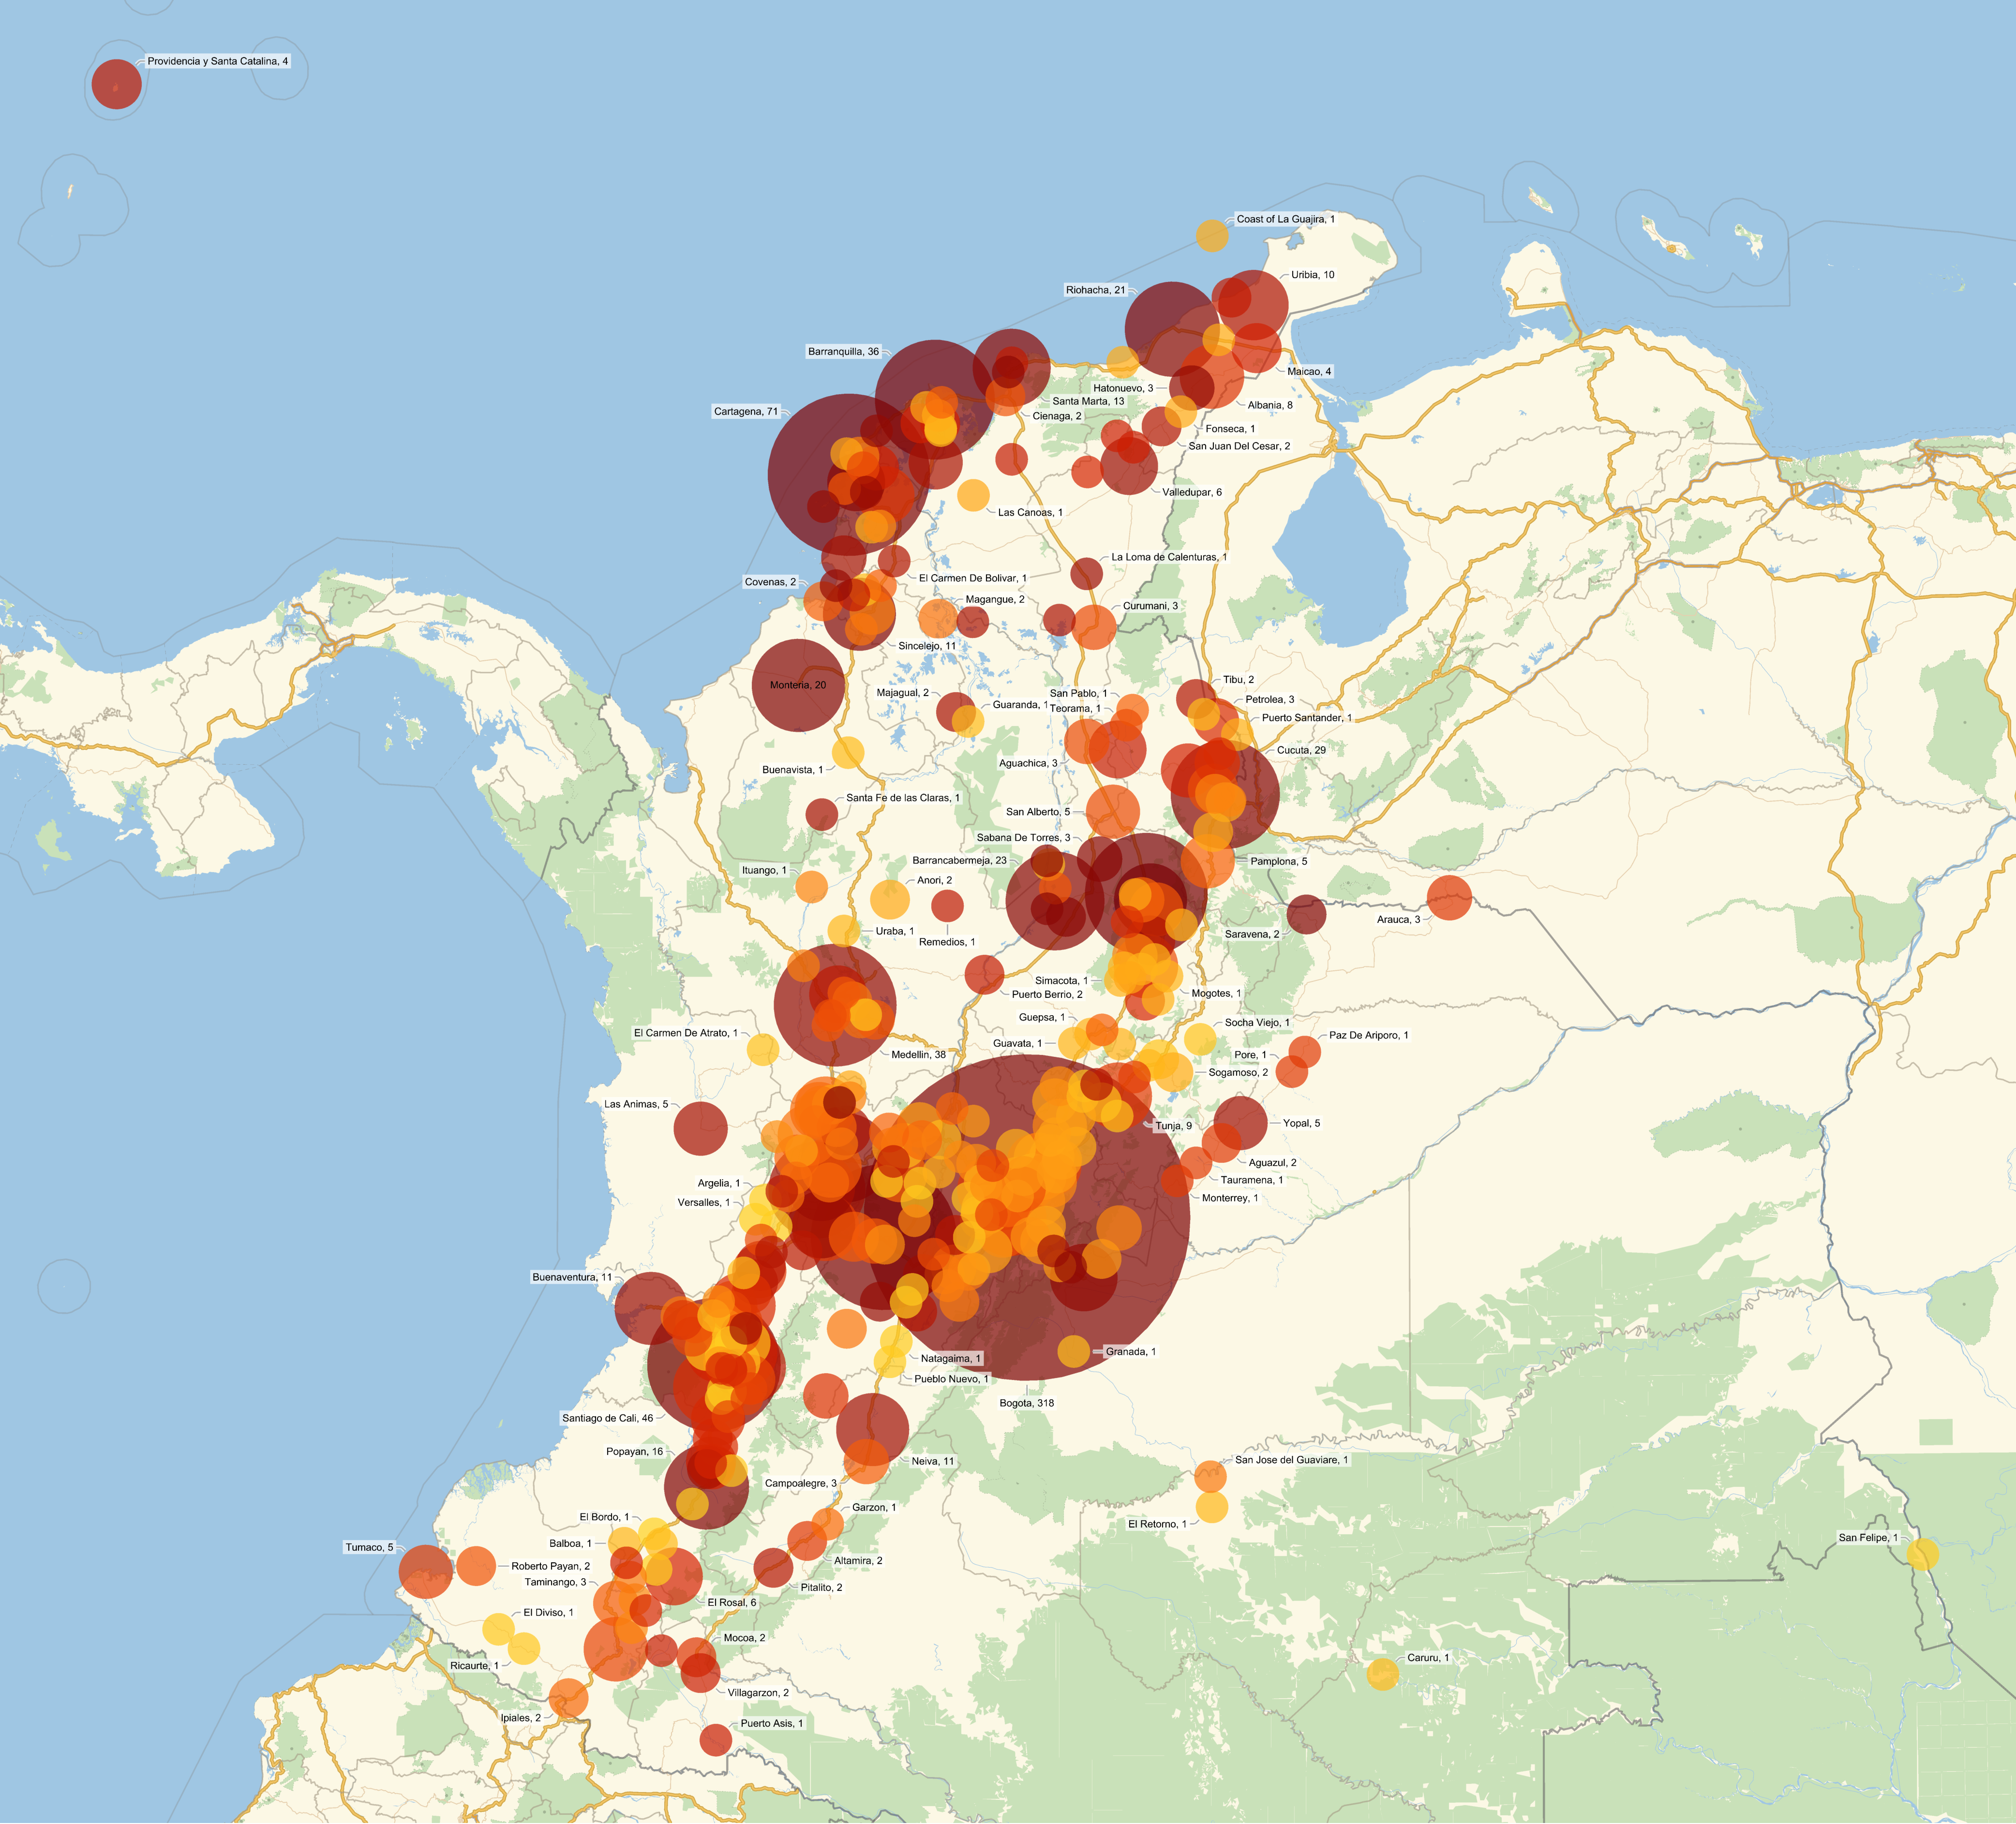
\includegraphics[width=1.0\linewidth]{pic/chart_peaceful.pdf}
                    	\caption{和平抗议的区域分布图}
                    	\end{figure}
\clearpage
\section{四月份与七月份税收目录}
\textbf{[四月份税收草案的目录]}
\par 第一编:重新定义财政规则,将其作为实现公平可持续性的工具
\par ·第一章:财政规则
\par =第一节:财政规则的参数
\par =第二节:自治财政规则委员会
\par 第二编:加强和确定社会支出的目标
\par ·第一章:实施团结收入计划以消除贫困和极端贫困
\par ·第二章:其他投资和社会支出机制
\par ·第三章:支出方面的紧缩和效率措施
\par 第三编:税收和环境负担的再分配的公平性
\par ·第一章:税收负担再分配的公平性
\par =第一节:增值税(IVA)
\par =第二节:增值税(IVA)豁免
\par =第三节:所得税和补充税
\par =第四节:个人所得税
\par =第五节:法人所得税
\par =第六节:临时团结财富税
\par =第七节:作为所得税和临时性团结财富税的补充的税收正常化税种
\par =第八节:临时高收入团结税
\par =第九节:税收程序、正式职责和处罚
\par =第十节:车用汽油和ACPM附加费
\par =第十一节:杂项规定
\par ·第二章:环境负担再分配的公平性
\par =第一节:减少对气候变化和污染的脆弱性的工具
\par =第二节:国家碳税
\par =第三节:对用于包裹、包装货物的一次性塑料制品征收国家税
\par =第四节:农药的国家消费税
\par =第五节:国家车辆税
\par =第六节:首府城市的收费
\par =第七节:单一能源解决方案基金
\par 第四编:补充规定
\par ·第一章:预算措施\vspace{1em}\\
\textbf{[七月份税收草案的目录]}
\par ·第一章:收入措施
\par =第一节:税收正常化 税收对所得税的补充
\par =第二节:所得税
\par ·第二章:反逃税机制
\par ·第三章:紧缩开支,提高效率
\par ·第四章:加强社会支出和经济复苏
\par =第一节:团结收入计划
\par =第二节:经济复苏措施
\par ·第五章:作为公共财政可持续性机制的财政规则
\par ·第六章:最后条款
\section{访谈稿}
\subsection{Camilo Mundólogo访谈稿}
\par (1)访谈时间:2022年2月25 日
\par (2)访谈地点:线上
\par (3)记录者:姜雨玥
\par (4)访谈方式:集体访谈(网络访谈)
\par (5)受访者基本信息:
\par 姓名:Camilo Mundólogo
\par 年龄:36岁
\par 职业:作家
\par 住址:现居北京(20年至今大部分时间在中国)
\par 家庭状况:父亲是产业工人和牧师,母亲是护士,总体经济状况良好
\par (6)访谈实录\\
\textbf{Politics}\\
Question: Do you have confidence in the current government of Colombia? From 0-5, could you please give us a score and explain the reason?\\
Answer: A lame 0. The thing is that the government didn’t start in a trustworthy way and the whole development of the decisions that the government made during the past 4 years has been really difficult to accept for most of the people. In my personal opinion, I can’t trust the government and the background of the government is also really dark.\\
\\
Question: Do you have confidence in the police of Colombia? Could you please give us a score?\\
Answer: It’s kind of difficult because I think there’s some willingness to do good in the institution. But at the same time, certain officers or certain people inside the institution made things really bad. It’s difficult to trust the police, but at the same time we trust the institution itself. For example, if you talk to a policeman, that man probably will be a lawful person. But at the same time there’s some kind of distrust because a great majority of the officers don’t act according to the laws. It’s difficult to answer but I will say a 1 and I’m still giving the chance for that answer to improve.\\
\\
Question: According to you, is corruption the main problem of the police department?\\
Answer: I think that there’s corruption in the institution. But at the same time, the values and the principles of the institution are based on respect and democracy. So when you get in to this kind of predicament that you trust the institution and the values of it, but at the same time there’s so much corruption and so many people inside it that make things looking really bad.\\
\\
Question: What is your opinion of the 2022 presidential election? What’s your opinion about Gustavo Petro, Sergio Fajardo and Rodolfo Hernández.\\
Answer: First of all, this election is quite a difficult one. (I guess that all the presidential elections in Colombia have something really concerning for the people, because there’s always some of a big deal to ) The election this year is very important because in one hand you have the people more and more uncomfortable everyday with what is going on not only in Colombia but also in the neighboring countries which is a critical situation. On the other hand, inside Colombia and its borders, the last 20 years have been really difficult because the democracy has turned into some kind of not really a democracy what probably could be in the 20th century. But now there’re other powers, not only the people or the institutions and the dark power behind the institutions that manipulates people. So right now the things to be decided in this election are really delicate. About these candidates you mentioned, Gustavo Petro has been a great figure during the past 20 years or so. He’s had a great political career and has also been fighting against many dark powers. Thanks to him, his political willingness, his intelligence and his investigations, we got to know a lot of things that probably were hidden by the institutions but people deserve to know. He has built confidence among the people and he has earned people’s trust throughout the years. Sergio Fajardo is kind of a confusing person because he has this kind of educational speech and his always talking about education. The thing is that his ideas lack of argument. He’s a renowned teacher and once was the mayor of some cities. He also has a great background. But the other thing is that his speech is always flat. He’s not confronting the real issues in Colombia. He never goes to the point while Gustavo Petro does. He’s totally the opposite of Gustavo Petro. He wants to give this image of (himself being) correct and the rightful person. But at the end of the day his whole image seems a little fake. And it doesn’t get much impresion of a trustworthy person. And Rodolfo Hernández is someone that just appear in the political scene. At the beginning of his career of being the mayor of Bucaramanga, he gained a lot of followers and a lot of people paid attention to him for the way he treated corruption and faced certain issues that needed to be faced in our country. But since he started with this presidential election, we get to know more about him. And also his latest media appearance has made it diffucult to understand his ideas. That guy sometimes doesn’t make any sense of what he’s saying. And the latest thing I’ve heard from him is that he was asked to talk about some province in Colombia which probably is one of the most forgotten by the government and not many people know about the province. He didn’t know how to answer. He just acted like he was talking to some fan or some follower in the street. But he couldn’t give a reasonable answer. For me and many other people it was disappointing that he didn’t know about that province. So I guess Rodolfo Hernández is not a good candidate for the presidency in Colombia. \\
\\
Question: What is your opinion of Uribe? What is the influence of him on Colombia? El País said that Uribe is the political shadow of Colombia, what do you think about the statement?\\
Answer: Uribe represents part of our history in the last 20 years or more and sadly in a nefarious(?) way. Because I think at the beginning he seemed to be a strong politician with strong values like he represented a great deal of Colombians’ way of thinking. But throughout the years, things have been changing. And that kind of thinking is everyday falling behind because the new generations want something different for our country. One of the things is that when Uribe was president, a lot of dark things happened in Colombia. There was the situation of civil war in Colombia since the 1950s. Later the army understood that they couldn’t face the situation with illegal armies. So many people in the countryside started to create another illegal army calld paramilitaries. Those paramilitaries started to face the other issue that was the first situation with the illegal army(?). So the thing is that after tons and tons of investigations, we now find out how Uribe was related to the creation of all this kind of illegal armies. And the way his party has been manipulating the public view and the way they’re still doing a lot of horrible things to the people. And many things that happened in Colombia during the past 20 years have been because of Uribe and his people. The thing is that Uribe has represented one of the darkest moments in our history. We don’t know if this is gonna end in any time soon but probably this could end or at least start to vanish in the next presidential election. But they still have a lot of power and a lot of money from all the killings, from all the land they stole and from all the drugs they have sold. They still have a lot of powers. So it’s been like a really dark moment for Colombian history.\\
\\
Question: Do you think the status quo has been better since the Peace Deal was signed?\\
Answer: The Peace Deal represented the hopes of many people. I have felt it like a fresh wind of hope because I grow up watching the news about all these killings, all these horrible situations and my family was even the direct victim of the war. My mother’s parents were killed around 17 years ago. Many people of Colombia have been victims of this war. When the Peace Deal was signed, as well as many others, I felt that could be a change and a different path. In fact, the different path was taken, but with this government of Uribe’s side, they don’t want a different country. They want to keep getting money from the war. It’s been a different situation and a different problem since the Peace Deal was signed. Because before that, it was clear who and who was the the enemy. But after the Peace Deal, many other situations started to come up. Because all the time the news has been saying that the main problem of Colombia is the war with the FARC, which was the most powerful illegal army that was fighting the government. They have been saying that all bad things happened in Colombia were because of that(the war). But when this illegal army and the government were williing to sign a peace deal, a lot of other things started to come up. And then people started to realize that the war wasn’t the problem. That war was the result of a bigger problem that existed before this war. Then things have started to change. A lot of other institutions were created thanks to the Peace Deal and older people started to feel that it’s been a slow, step by step situation that people started to understand the power they have and why they need to participate in every decision, otherwise the war situation will never end. So many things have changed since the Peace Deal, but still the “bad guys” are trying to destroy that peace deal. I think that’s also a reason why there were so many demostration and protests in Colombia during the past 2 or 3 years. Because somehow people are tired and really want this to change. \\
\\
Question: Do you think it is reasonable for the government to spend more money on armies because of the existence of such threat to people?\\
Answer: Definitely not. The Colombian government has been spending a lot of money on all the armies and all these “killing systems”. They(the armies) have been receiving a lot of money all the time and that also has been taking the resources from all the other important parts of our economy and society, like specifically the education. Thanks to the Peace Deal, we start to see that education is important but why all this time the government just put money into the army and no money for schools, colleges and universities? So there’s no reason to accept more money in the army. And now this is the situation. By the way, another illegal army that is now causing so much trouble is the ELN. This illegal army is also willing to sign a peace deal, but I think the situation with them is more complicated. Definitely the army has enough money and enough tools(?) so they don’t need any more.\\
\\
Question: Gustavo Petro was once a member of the guerrilla groups. Does that experience influence people’s opinion towards him?\\
Answer: Definitely. On one hand, in my personal opinion, that experience made him more capable of understanding the difficult situation in our country. Also I think we can take it as a good example that the former president of Uruguay, José Mujica, was also member of a illegal guerrilla. I guess that the new Chile president was also member of some kind of group. But Gustavo Petro was more like someone in the “ideology” part but not so much in the “killing” part. I guess that experience gave him a lot of understanding of the way things happened in Colombia. But on the other hand, you have to understand that after all these 50 years of war, people tend to just assume one side or the other. It’s more like a bidimensional way of thinking. If you were a guerrilla member, people will think that you were a butcher, a killer, a rapist or other things. I think many people still don’t understand the way that things happen. Also a lot of people in Colombia don’t understand why we’re in such situation right now. They might think that Gustavo Petro was once a guerrilla and thus a bad person. Most of the people that have a bad impression of Gustavo Petro have never listened to any of his speech or interpretation(?) in the Congress. I have some family members who just think that way and don’t listen to his speeches or to investigate and go deeper. They just have this two-side mindset and stay on the surface. It’s really sad that some people think that way.\\
\\
\textbf{Reform and Protests}\\
Question: What do you know about the fiscal reform? Are you against it? Why?\\
Answer: The thing is that our Congress has a lot of people(officers) that don’t work for the people. They just work for coorperations and even the illegal groups that have a lot of power. Usually when they make this kind of reforms, they just want to keep taxing the common people and keep getting money out of everybody. In Colombia, every year 5 billion pesos are stolen from the people and the government by corrupted officers. So when the government is running out of money, they just make up this kind of reforms and they want to get money from the common people. It’s kind of crazy that they keep “milking the cow until the cow has no milk”. That’s basically what happened with this reform. The government is broken because of the COVID-19, the Venezuela migration crisis and other things. So they’re going to put more taxes, and the people want to end (all the taxes). If you see the situation on the streets, you’ll see a lot of people with (失业,没有财务能力维持生意和生活) Basically the only people that are getting money are people with some kind of relationship with the corruption or illegal groups. So basically the people that were protesting during that time were the people in hunger and tired of all the situation. \\
\\
Question: What was the demands of protesters in 2021?\\
Answer: I guess in Colombia people are probably not that aware of the history of Colombia and Latin America. They know something bad has been happening all this time because there’s no way to explain how bad the situation is now. Because for most of the people, that’s all the things they saw during their entire lives. Somehow I think everything always reaches to a point when there’s no return. So I think many different sides have come to the same point, like (the lack of) social justice, the economy breaking down and the government corruption. I think if you ask the people on the streets who’re living out of what they can get (by protesting) on the streets, they will just say that they’re tired. I guess that every citizen in Colombia trying to make a living in a good way, no matter rich or poor, is tired. \\
\\
Question: Did the protesters’ demands change during the period? Did the responses of the government change the process and the goals of the protest?\\
Answer: It’s difficult because one of the things that the protest left everyone with is that somehow people need to work and can’t live in a protest. But I think that people still believe in institutions and that things can change in a proper way following the democracy procedure. I think after all these years with the war, the killings and all the bad things, people still believe in the institutions. So probably the government or all these corrupted politicians understood that they couldn’t mess with the people any more. They even tried to find some other ways to manipulate people’s minds and to generate confusion. I think it’s kind of difficult to answer for me. Probably you can say that we didn’t get any result, but I think one of the greatest results of this protest is that people were more aware of their power and more aware of what they can do to remove government’s decisions by protesting.\\
\\
Question: What do you think of the violent conflicts between the police and the people? Were there more violent protests than peaceful ones?\\
Answer: There were more peaceful protests. As I heard from all the information on social media, violent protests were basically a provocation created by the police or the government. There were more peaceful protests.\\
\\
Question: Some people say that la Primera Línea is a group of terrorists that conduct violent actions like breaking into banks. What do you think of it?\\
Answer: I think la Primera Línea was the result of protesters’ organization. It was more like a citizenship organization, more like people coming to terms of what they’re doing. Definitely they’re not terrorists as we know what terrorist means. But the people that usually call them terrorists are the people who want to manipulate people’s mind and want to create all this confusion. But at the end of the day, I guess we all know that they were just doing what they had to do, which was to defend their ideas and the principles or values of democracy although in a violent way.\\
\\
Question: Do you think that guerrillas and other armed groups participated in or even organized some protests during that period?\\
Answer: I find it really hard to believe. Because they have different ways to operate. And the thing is that these guerrillas or illegal groups have been fighting for a long time and what was going on the streets was probably more like a popular reaction to the current situation. It was more like people’s reaction but not something related to illegal groups. It was hard to prove that there was any connection with illegal groups since that kind of thing has been said only to deminish and cease what people really want. They told every citizen that some groups are terrorists just because they’re defending their point of view or they’re against the methods taken by the governmet. Usually the government says that kind of thing just because they don’t know how to face the real problems. They just want to criminalize the citizens.\\
\\
Question: Do you think that police violence caused more protesters to behave violently or the violent protests forced the police to fight back? Are there any cause-and-effect relationships?\\
Answer: I think the police were mostly the ones causing people’s reactions. Because sometimes people are stopping the traffic or doing some kind of demostration and the orders that police recerved are to move those people no matter what they(the police) have to do. Eventually there’s going to be a confrontation between the people and the police. \\
\\
Question: After the protests, have anything changed in people’s lives? Do the government implement what people’re asking for? Do you think the protests have been useful?\\
Answer: Things have changed but not percisely in a good way. I think the police keeps acting in a really un(?)lawful way and the government is still doing what they do which is giving contracts and work to people not prepared for what they have to do. Basically the economy keeps going down. Probably what happened in 2021 hasn’t finished yet. Probably things could get worse but who knows? With the next presidential election, if the president is a person that can deal with the matters that need to be solved, probably things can change in a good way. But so far I think maybe the situation is just a little more calm but not resolved or things have changed better. Things keep getting worse.\\
\\
Question: During that period, did you often receive reports of the protests on social media? Were the contents of them different from what people experience in real life?\\
Answer: The thing is that in Colombia you can probably get the most reliable source of information on social media. Probably some of the newspaper can give some information from a trustworthy source, but there’re others who twist the information and make people look like the ones who caused all this damage and terrible situation. I like to get information from different sites to see what things are really going on. \\
\\
Question: Do you think corruption is the biggest problem of Colombia? What can the government do to stop the situation?\\
Answer: Definitely corruption is the most horrible cancer of Colombia. It’s been really difficult because it’s almost a part of everyday life. I think it’s not only a government issue or a government’s task. It’s also (something) that needs every citizens to permit to change. Definitely, if the government wants to do good to change, they need to make a big clean in every institution. Every institution needs to be reset, especially the legal institutions like the law institution. Every institution in our country needs to expel all kinds of corruption.\\
\\
Question: Are those projects of opening datas of great help to the situation?\\
Answer: I think something that the government has been doing all the time has to go deeper than that.\\
\subsection{William Andres Betancourt Villota访谈稿}
\par (1)访谈时间:2022年3月5 日 
\par (2)访谈地点:线上
\par (3)记录者:姜雨玥
\par (4)访谈方式:集体访谈(网络访谈)
\par (5)受访者基本信息:
  \par 姓名:William Andres Betancourt Villota
\par 年龄:23岁
\par 职业:学生(公共管理专业,取得过西语和英语教学资格证)
\par 住址:Sandoná, Nariño
\par 家庭状况:贫穷,月收入低于最低工资
\par (6)访谈实录\\\\
\textbf{Politics}\\
Question: Do you pay close atention to the political issues in Colombia?\\
Answer: We have a government that doesn’t understand the situation that people have to live. We have, for example, a minimun salary of 250 dolars and the economy is so devaluated. The prices of the products are so high that you couldn’t buy many things. It is the first situation. The second is that the young students don’t have the posibility to stay at the university. It’s easy to enter a public university, but it’s difficult to stay because you have to pay for your rent and your food. There are people who live in small towns but have to move to the principal cities to study. So we students of university try to get some resources and money to stay and to graduate from our program. Another thing is that, I think, the power is in five or six riches families of Colombia. The corruption is incredible because they buy for the gold and have many strategies to put a president and the senators. It is complicated because if you talked about that, for example, you said that someone is buying votes, you could be murdered. So here in Colombia we have social leaders killed everyday for talking about the environment, politics and the corruption. \\
\\
Question: Could you please tell us by what means do you usually get such information? Do you search for such topics or simply receive news and reports in your daily life?\\
Answer: I just receive such information. Because as I said, it is complicated to be a social leader and to talk about these situations for that your family or you could be murdered. There are some TV news stations that don’t belong to the government but their owners are the friends of the president. They produce fake news or don’t say everything. We have some social medias on which we can see videos, images and understand the situation how the government works and doesn’t work in some parts of Colombia.\\
\\
Question: Do you have confidence in the current government? From 0-5, could you please give us a rating score? Could you please explain the reason why?\\
Answer: I think 1. The president and his group, the senators and the ex-president just want to get money. It doesn’t matter if they sell a mountain or a páramo where many people get the water. It doesn’t matter if the people don’t have more money(mountain?). Another thing is that they sometimes ask the police to kill people or use force to intimidate students in a strike. They don’t respect the human rights. They don’t think about the people. They just think about getting money and it doesn’t matter if they have to kill someone, sell any nature resource or something like that. \\
\\
Question: Is police violence a very common phenomenon in Colombia? Do you know anyone that has been victim to police violence? Do policemen often conduct violent actions?\\
Answer: Yes. I study in a public university in the city. I have some friends who have led the strikes or mobilizations and other activities. Some of the activities are cultural like dance, art and performance at street. And then they’re caught by the police and sent to jail for one night or one week. I have a friend who lost one eye because she got a stone or metal piece against her head. In other places like the capital or other states bigger than mine, things are more complicated because there’re people or students killed. Obviously they tried to say that they didn’t do it on purpose, but we know that the reality is totally different because here in Colombia there are and were some guerrilla groups. Since we’re now in the peace process, many groups left. But they’re killed after some years, we don’t know by whom, but there’re some paramilitary groups or the police but they said that they were cleaning(caming?) out people like that. But in Colombia you have to talk about that you could be killed.\\
\\
Question: Are guerrillas and organized armed groups still a threat to your daily security?\\
Answer: Yes. The biggest guerrilla that took part in Colombia for many years was the FARC. In Cuba they have the peace deal made by the last president. And they leave these groups but they have some conditions like, for example, to get five positions in the senate of Colombia, to get salary and something like that. But this president have difference with the actual president, so this president, Iván Duque, has try to eliminate the peace process. For that, many ex-guerrilla groups try to create new groups like the ELN. They are in the mountains of Colombia and control the traffic and drugs. This is like a inter-conflict between the militaries of Colombia and the guerrillas groups. So if you live in a town where the guerrillas exist, you could be murdered or accidentally killed in a war, so it’s complicated.\\
\\
Question: Do you think it reasonable that the government should spent more money on the armies because of the existence of guerrillas?\\
Answer: Yes. Because the government here in Colombia get the majority inversion of the money in the war. We try to fight for that because we need more money in the health service or in education because we don’t have a good health system in Colombia. But I think that they are not trying to talk with these groups, just kill them and kill them and kill them. If there’s a community near to these guerrillas groups, many of them are killed or, for example, if the try to eliminate the cocaine with a chemical that causes cancer. Many people who live in towns and small villages don’t want the government to use this chemical because they don’t have drugs but could get cancer. \\
\\
Question: In your opinion, what is the biggest problem in the current government of Colombia?\\
Answer: The biggest problem in the government is the corruption. We have ministers but many of them took a lot of money. For example, the last scandal was from the Minister of Technology who said that she was going to put internet in some schools but took the money and is living abroad now. They try to dissimulate the situation, so I think the biggest problem is the corruption.\\
\\
Question: And what do you think might be the solution to this problem?\\
Answer: I think that it’s really difficult to eliminate the corruption in Colombia, but we have to try to vote for new people who try to defend the human rights and know how people in small towns live. In the last election there was corruption because there were some votes not counted for the opposite of the actual president, or people had to vote for the actual president if they didn’t want to lose their jobs in private and public companies. It’s complicated. So I think that the way to change the situation is to try to vote for alternative(?) people and be careful with the election. We have to vote next week for the senators, so we have to try to think and don’t receive money to vote for someone.\\
\\
\textbf{Presidential election}\\
Question: What is your opinion towards the 2022 presidential election? Among all the candidates, who do you support or extremely dislike, and why?\\
Answer: We have an ex-president called Álvaro Uribe Vélez. He decides who is going to be the next president. So the last president and the current one are for him. They are like the same political line. They have been growing in power, in money, in companies and in people. I support Gustavo Petro who is an economist and comes from a poor family. He understands the situation of Colombia. He has been defending because he was senator. So I think that he is a good person and has some senators who are working for people and for poor people to get more opportunities to study and to get a job. Because when we want to enter a university, the easy way is to go abroad. In Colombia you could get a job, but it’s just for hours or you don’t have a good salary to live in the situation. I support him but we have to wait because now there’re like 20 pre-candidates for the president, but in May, there will be just 2 options, 2 with the most votes in March 13. I think that he’s gonna be in the second round so we are going to try to vote for him because, otherwise, the ex-presidents and the richest families in Colombia are going to join to vote for the opposite of Gustavo Petro.\\
\\
Question: But Gustavo Petro was once a member of the guerrillas. Does that experience influence people’s opinions towards him?\\
Answer: There was a group, M-19, it was created because one year the election was corrupted because, my parents and grandparents told me that, in the evening, they anounced a president. And then in all Colombia the lights turned off. But at 6 or 7 a.m. the next day they anounced another one to be president. It was obvious that they controlled(?) the election. And this group(M-19) was created. This group was formed by students of the national university studying economies, laws, medicines and many of them...(连接有故障) The right-wing forces in Colombia tried to convince people who didn’t do the study that he(Gustavo Petro) was a guerrillero. He belonged to a guerrilla group. So you don’t need to vote for him, because he’s socialist, he loves Hugo Chávez and Castro of Cuba. People believed in that so it’s really complecated because, for example, during the last elections they say if we don’t vote for Iván Duque, we are going to belong to another Venezuela. So people worry about that because the situation in Venezuela was difficult(bad?) with their president Maduro. People didn’t want to become Venezuelans. And now the election is very corrupted because they say if you vote for Gustavo Petro, Vladmir Putin is going to come to Colombia and kill people, but people believed in that we don’t have to vote for a former guerrilla member. But if you look back, these guerrillas were born because of corruption of the same people with being in power, in president in Colombia.\\
\\
Question: El País says that Uribe is ‘la sombra política de Colombia’. What do you think of this statement?\\
Answer: It’s true. As I mentioned, Uribe has the power to put a president. He (has some connections with the Narcos?) but he doesn’t admit that. He has some paramilitary groups who are the people that killed the líderes sociales(social leaders), the students and people who were fighting for their rights. He has a lot of money and is one of the richest men in Colombia. He has companies, businesses and illegal businesses. So he is like la sombra negra in Colombia. That is why young people especially don’t believe in him. We are trying to demostrate that he doesn’t have the same power that he had before some years ago. But the old people, the militaries and the police try to defend him and to support him. But I think that they’re worried about the election because (according to) the pools and votes in social media, Uribe’s candidate is in the last position. So I think that he’s waiting for the second round and he’s going to support (his candidate) and the traditional party is going to support one candidate to win this election and to defeat Gustavo Petro.\\
\\
\textbf{Economy}\\
Question: Are the prices of products in Colombia high compared to the average salary of Colombians?\\
Answer: Yes. \\
\\
\textbf{COVID-19 pandemic}\\
Question: Then talking about the COVID-19 pandemic, does it influence people you know when it comes to income and employment? Do you think that the pandemic made your lives more difficult?\\
Answer: Yes. There were people who could work in a virtual way, but there were people who lost their jobs. I think that the president couldn’t face the pandemic situation compared with other countries. For example, we are one of the last countries to get the vaccines. People without vaccines couldn’t go to the campus, the office or to work with others face to face. So I think that the pandemic affected the economy, but now they say that the economy(is bad) and the prices are high due to the students, the indigenous people and all the people who don’t agree with the government. They(the government) said because they(protesters) took to the street, they couldn’t transport food or other products so the prices are high. But it was a lie because nowadays there haven’t been strikes but the prices are still so high. For example, in my state, some regions produce potatos. Several months ago, these potatos were so cheap, but now they’re so expensive. This is because of farmers don’t earn money from growing potatos. They have to increase the prices and the economy for the families we have a 250 dollars salary per month. And you can’t buy a lot of products like you could before. \\
\\
Question: How much is the treatment cost of COVID-19 patients? Do you think they get enough help?\\
Answer: Nowadays I think that the situation is normal, we don’t have many people infected with this virus. But before, we don’t have good hospitals, people are going to die in the hospitals. The government doesn’t give enough money to the hospitals and the healthcare system. They got money and gives it to the forces, to the army and to the war. So it was complicated, but now if you get covid, you don’t have to go to the university or the office, but the government doesn’t give money if you’re infected.\\
\\
Question: Then have most people in Colombia already got COVID-19 vaccinacions?\\
Answer: Yes. The majority of us got the old vaccines, for example, during these months in Bogotá it’s not mandatory to use facemasks because the situation is going well. \\
\\
\textbf{Reforms and protests}\\
Question: What do you know about the fiscal reform last year? Are you against it? Why?\\
Answer: I was against the reform because the ministery didn’t know, for example, how much the eggs cost. Here in Colombia, 12 eggs normally cost 2 dollars. And the president and this mandatory said that 12 eggs were, for example, 15 cents. So they didn’t know the situation that obviously due to the pandemic the prices were higher than usual and they didn’t know that another thing was that we had been paying taxes all the time and we didn’t have good public services provided by the government and the public institutions in every aspects of our lives. So it was crazy to increase the taxes and something like that because the economy and the financial situations of Colombians were difficult at that time. \\
\\
Question: We’ve heard that one goal of the tax reform was to take some part of the income of the middle class and use it to help the poor people. Do you think it was reasonable?\\
Answer: No, it was not reasonable. It was another thing. The want the middle class to disappear: just the poor and the rich and no more. In the middle class there are, for example, teachers and some doctors who had to study and to (go through a very complicated path) to get a job. Another thing is that some international companies don’t pay a lot of taxes because they (create) some job opportunities(?). And micro-companies(?) or small businesses in Colombia have to pay a lot of taxes so they couldn’t expand their companies. So I didn’t agree with that (tax reform).\\
\\
Question: And a lot of people say that the social projects of Iván Duque only help a small amount of poor people and many others are still waiting desperately for help. Is that the situation?\\
Answer: Yes. It’s true. For example, there were some social programs like Ingreso Solidario, but the people who received them were very few. So Duque said that he was going to implement the tax reform to continue these social programs but it was not true because he was saying that basically all the Colombians can receive help from this subsidio(补助金) but it wasn’t true. \\
\\
Question: What is your opinion about the Proyecto de Inversión Social(社会投资计划)?\\
Answer: It was Ley de Solidaridad Solidaria. He said that it wasn’t a tax reform but it wasn’t true because in my opinion the government had to get the money effectively(?) and divide it to some sectors. But to use these programs, for example, you have to pay 30 dollars in taxes and the president is going to give you only 15 dollars. So it doesn’t make sense because you have to pay more and you’re going to receive a small amount of as a help from the government. So it was not a very good decision of the government.\\
\\
Question: We’ve heard that there were 2 tax reforms and the second one was in September, 2021 and it was more commonly received than the first one. Do you know the difference between those tax reforms and the reason why people prefered the second one?\\
Answer: I’m not really sure about that but I think that it was because that some senators tried to modify some things to make lives of poor people better. But when it took place I wasn’t in Colombia but in the US, so I didn’t have more information about that. \\
\\
Question: In your opinion, what were the demands of protesters in 2021?\\
Answer: I know there were other situations. For example, we want the cero matricula because many people lost their jobs: parents lost their jobs and students lost their partial jobs. You have to pay for the Internet, the computers and many other things for virtual studying but the government doesn’t care about that. So I think that was the reason. And the healthcare system in Colombia (is also bad). We don’t have enough hospitals to attend to people who were infected with COVID-19. \\
\\
Question: According to your perception, did the protesters’ demands and aims change during that period?\\
Answer: Yes. For example we got the Matrícula Cero which means that if you study in a public university, you don’t have to pay for your studies. Before that I had to pay 100 dollars although I study in a public university. But now I don’t have to pay because due to the strike and the protest of the students, the government decided to pay the fees and everything for us. It was the first one and the second was they don’t accept the first tax reform. I think that the mobilization, the strikes could change that at least. \\
\\
Question: Did the responses of the government change the process and goals of the protest?\\
Answer: Yes. For example, they used the ESMAD, which is like a group of police in Colombia, so they used their repression and their force to avoid the strikes and the mobilization. But I think that there were more people in the mobilization than the police group, so I think that was why the government had to accept the reasons why we were fighting in the strikes of last year. \\
\\
Question: Do the protests have a strong impact on your life? In what aspects? Could you please give us some examples?\\
Answer: People joined (the protest) for a reason. People have the power and the change(?). So I think that it’s our task as young people to try to change the minds of the old people because they, or the majority of old people in Colombia, didn’t have the opportunity to study and the main information source that they have was the news. As I said in the beginning of the interview, there are some news station or TV channels belonging to the president’s friends, so they don’t tell all the truth. They try to give an image that the government and the president are doing their jobs well and are thinking about people but it’s not true. So I like the Pacific Mobilization and the culture of the mobilization to try to take the attention of the government and the president and to try to change because we are the majority while they’re just few people, the richest people in Colombia. But we, the people of the towns in Colombia are the majority so we have the power to change and to continue changing these bad situations in Colombia. \\
\\
Question: Were there many violent protests last year? Did they involve with violence in the very beginning?\\
Answer: Yes.\\
\\
Question: Do you think that police violence might have caused more protests to end up with violence?\\
Answer: Yes. The police used violence to intimidate people in the streets and in the mobilizations.\\
\\
Question: Some people say that many organizations like la Primera Línea are terrorists because they conduct violent actions. Many people say that they only wanted to work normally but the protest prevented them to work. What do you think about it?\\
Answer: I don’t agree because, I don’t belong to la Primera Línea but their violence was like an respond. If they(the police) attacked with violence, they responded with violence. For example, in many Pacific Mobilizations and protests, they(the police) used the tanks and other arms, but there’re not organizations protecting the Colombians who joined the protest. I think that we have to protest in a pacific way, but in a revolution or in a strike there are so many ways to demostrate that we don’t agree with the government and the system that we’re immersed. So I think that they might have smashed something like the streets or some monuments, and then the government had to pay for those expensive things and they said that was why the prices were so high. Also some infiltrados(渗透) police pretended to be students and sabotaged the streets and other structures. This was like a strategy that the government said the students were bad people who destroyed everything while the police were the superheros of Colombia.\\
\\
Question: Some people say that guerrillas and other armed groups participated in or even organized some of the protests. Is that true?\\
Answer: Yes. I think that there were some infiltrados even with the police and the guerrilla groups. There were some students who were immersed in that revolutionary ideology or something like that. For example, they received some arms or guns from the guerrilla groups and some instructions to do that. I think it’s true. For example, in my university which is a small one I think it didn’t happen, but in some big universities it happened.\\
\\
Question: Did the guerrillas and other armed groups have the same demands with the majority of the protesters?\\
Answer: No. \\
\\
Question: After the protests in 2021, did the government implement what people were asking for? Do you think that generally the protests have been useful?\\
Answer: Yes. I said before that the government begin to pay university costs. It was the biggest achievement the mobilization got. But the farmers and the indigenous people haven’t received what they’re fighting for.\\
\\
Question: During that period, do you often receive news or reports of the protests on social media? What do you feel about that? Were the contents different from what you experience in real life?\\
Answer: Yes. In big cities like Medellín or Bogotá, the situation was more complicated than that in my state. It’s frustrating because, for example, there were some social leaders or student leaders murdered and nobody knows who did that. It was unfair because they were trying to change (the situation) and get more opportunities for Colombians but the government is going to forget them. Even people of Colombia will forget them. So it’s complicated. And there were some videos and images on social media deleted by the president and the government because they didn’t want to show the reality to the world. They tried to limit their influence. \\
\\
\textbf{Education}\\
Question: Do your university or the government of your region provide scholarships for students? And to what extent can those scholarships help the students and their families?\\
Answer: Yes. Many families have benefited from the Matrícula Cero. They don’t have to pay and there were some private universities which were asked to offer scholarships and discounts in the tuition but it was impossible. I think that families can benefit from the Matrícula Cero.\\
\\
Question: How is the popularization of higher education in Colombia? Do most people have the opportunity to get high-quality education in their own regions?\\
Answer: No. For example, here in my state, there is just one public university. Everyone in my state wants to enter this university. So we have to take an exam in the last year of high school. You have to get high scores to enter the university. And there is a kind of credit that they give you money for all your career but in the end you’ll have to pay very high interest or taxes while the government should have implemented more projects and courses to help the students to study in private universities. Before, only rich people could study in private universities. But now, poor people have to take the credit and pay for 10 or 20 years after their graduation. It’s so complicated and we don’t have the same opportunity that people who study abroad have, like scholarships or residence in the campus. So for us, it’s hard to be professional and to find a job. \\
\\
Question: Did many student groups in your university participate in the protests in your region?\\
Answer: Yes. There were many people who participated in the protests but many of us live in towns so due to the pandemic you had to go back home. So it was difficult to go to the city and the streets to protest. But many people participated, not only students, but also parents and people who worked in different organizations. We were in a pandemic and people had to use facemasks, but even that people participated a lot in the protests. \\
\\
Question: How did the students who participated keep in touch with the organizers of the protests?\\
Answer: We keep in touch on social media. There were some groups of student leaders who organized the mobilizations and the strikes. They sent the information and details of the protest, like when to go and where to go, on social media. But we had to be careful because as I said before, some infiltrados who tried to be alert and to intimidate the students were also participating. For example, there were policemen who took pictures of your face and tried to identify you. \\
\\
\textbf{Future predictions}\\
Question: What do you think of the ecnomic situation in Colombia? Will it progress in a year from now on? Will the prices of the products be higher, or keep the same, or be even lower?\\
Answer: I think that we have to wait for the new president of Colombia. Because the current president Iván Duque is going to finish his term in August, we’re in the last government of him. And I think that we have to wait for how the new government is going to work, what are the projects that they’re going to have. I think we have to wait for the new elections.\\
\\
Question: Y bueno, queríamos saber ¿cuál es la proporción de su gasto educativo en el ingreso total de su familia?\\
Answer: Bueno, en ese momento terminé una carrera y ahora estudio una nueva, que es la administración pública. Entonces por ejemplo mis clases son desde seis de la tarde hasta seis de la noche. Entonces yo estudio aquí de noche, y ya no hay servicio público de bus que es más barato, que es medio dollar. Entonces tengo que utilizar el taxi, que generalmente son dos dollares o un dollar y medio. En pesos colombianos son como de seis mil a ocho mil. Entonces creo que esos son como los más gastos, también pues como un snack, como un refrigerio, en medio de las clases, ¿sí? Entonces yo creo que sí igual con mi abuela y pues ella hace unos productos como de ropa de bebé, y es tejidos, entonces es que ahorita la situación pues económica, como lo mencionaba, con los precios tan altos y la economía tan devaluada con el peso colombiano, pues se ha vuelto como más complicada la situación pues de los gastos diarios, y además accede pues el servicio educativo, como lo dije a través de las luchas sociales alcanzó lo de la matrícula 0, que era pues antes pagar cien dollars, que eran como 400,000 pesos colombianos. Con estos de las movilizaciones alcanzó la matrícula 0 , no tenemos que pagar matrícula, pero pues hay estos refrigerio o las fotocopias, los libros, el transporte pues principalmente para regresar a casa a las seis de la noche, que son los gastos más se perciben, que un poco complica la situación.\\
\\
Question: Entiendo. Entonces ha mencionado que estaba en los EE.UU., y ¿esto es por motivo educativo o por otros?\\
Answer: Sí, yo soy en un programa de enseñanza de inglés en español, entonces fue como por motivo tanto educativo como laboral. Una oportunidad de trabajar en un campamento de verano, entonces estaba como estar en contacto todo el tiempo con personas que hablaban ese idioma, inglés, como primera lengua. Y de la oportunidad también como enseñar español a algunas personas o niños que estaban interesados, entonces fue más que dos, y como pues por parte de la universidad y como algo educativo. Y laborar a la vez porque pues me los pagaba por eso. \\
\subsection{Airi访谈稿}
\par (1)访谈时间:2022年2月15日
\par(2)访谈地点:线上
\par(3)记录者:邱文治
\par(4)访谈方式:集体访谈(网络访谈)
\par(5)受访者基本信息:
  \par 姓名:Airi (Suarez Gama Heidy Catalina)
\par 年龄:17岁
\par 职业:学生(Colombo American school 高中毕业,正在大学申请)
\par 住址:Bogota(也在乡村Firavitoba小镇居住)
\par 家庭状况:中产及以上(父母都是工程师,父亲是电力项目经理,母亲在外企任职)
\par 其他信息:英语水平非常高,学习中文并准备留学,成绩优异,有一个弟弟
\par (6)访谈实录\\
\\
Q: Can you tell us the economic situation of your family? Where would you put your family in the society, relatively rich, medium or poor?\\
A: my family economic situation is kind of that average. You know in our society we can be divided into 6 sections. We have that the first one and second one which are the poorest. They don’t have the energy, weather, or any other basic services, they are not provided to them. So according to the bills and eh energy bills, the government they said which class are you in, so my family is classified as class no.4, almost medium class. It all depends how many people in your family were and how many of them get a salary or a wage. Right now it’s only my dad working in the family, my mom stop working almost a little before the pandemic so I will say I’m in the middle class.\\
\\
Q: Do you pay close attention to political issues? Give us a number describing its extent, from minimum 0 to maximum 5. By what means do you get relevant information? Do you think you are concerned about such topics actively or rather passively? \\
A: I’ll put a 2. Because actually I am not ware about the political issues in my country unless it is very very big, and it mostly because my country is highly politized so taking these tends political situation is kind of (). I prefer just to, like, put myself at work or daily topic lifestyle, and where do I get information basically from social media. Though I also watch tv and the news some staff, but those are also polarized, tightly polarized, They always take a stand, whether it's a liberal or conservative place. And so the information they provide is not very accurate. So I prefer listening to different people's opinions and twitter and getting to know more about it.\\
\\
Q: since I know that you hate Gustavo Petro very much, so what is your opinion of the 2022 Colombia presidential election? What´s your opinion about Gustavo Petro, Sergio Fajardo y Rodolfo Hernández? And other candidents?\\
A: (我觉得我不太适合回答这个问题),I haven't been as much aware from the presidential elections this year since they haven't even started their official campaign by now. However, I think regarding Gustavo Petro, as you asked, many people think he might be the worst candidate out there. Since he has been proven to have some relationship with the guerrillas and that stuff, it's kind of hard to people to believe him and like believe he will make a change for the country, and he will not take advantage for himself. But I see there are two parts because he has relationships with the the guerrillas and that stuff but people. But at the same time, he has done a lot of improvements for our country in regards to those exact problems. So he began some appears discussions between them and some also public transportation advancements advances in that aspect. so It's kind of neutral. But I wouldn't go for Gustavo Petro if asked. There are a lot of new candidates. For example, we have one who was also a candidate 10 years ago, and she was a girl, she's cool I forget her name. But she was captured by () for almost 10 years. And now she's running again for this election. So I think she has a lot of experience in that aspect and she could be a great candidate. Also it would be really, really cool if she a woman could be the first woman president of our country.\\
\\
Q: What is your opinion about Uribe? For you, how is the influence of Uribe on this country? El País says that Uribe is “the political shadow of Colombia”. How do you view this statement, and why?\\
A: He has the worst reputation, indeed. And it is because the way he speaks and the way he presents his political campaign is really hard. And he's been in politics almost since his childhood, his grandparents were also in politics. His whole family has a whole influence on my country's politics. So for example, this last 4 years, our president was Ivan Duque, but many people say he was controlled or and by Uribe, he was his puppet, because same ideas were transferred to you, and he was the one who did all projects and stuff, but it was all Uribe’s idea. And so he might be the worst reputation, but no matter if he wins or not, or if he has any place in the politics, he still can get a lot of influence and other people get his ideas through that way.\\
\\
Q: Do you have confidence in the current government? From minimum 0 to 5, give us a score. Why?\\
A: I'd say 3. Since it depends on the situation, because when our country's relatively calm and the situation is not as bad, then the government does pretty good job, but this is my perspective from a medium class. If we go and see the situation from the lower classes, we can come to see there's no water, there's no energy, there's no education. We also have this “高考” but we call it ICFES. It's our college entrance examination exam.
I saw yesterday on the news. I want to say “记者”, The reporter, the reporters that the reporter said that the lower classes had a really, really low like points in that exam? It was because the pandemic they didn't have access to any internet. So mostly like first, second, and third classes, they were literally out of, They were rub their feature opportunities to get into a good college, just because they didn't have any good internet. And that's a thing that's a basic service. I think that the government should take care of. So it's kind of the government thus a pretty good job when the country is stable. But if we got like, come to see my country situation in May and March last year, when there were many parties and there were many people are fighting for our rights and for doctors rights, doctors wages, for education, and many people just got together to fight and fight for our rights. But basically, our precedent didn't know what to do. He was just () as the way to say it. He has never seen so many people against his government, against his politics, against this crazy rise in taxes he proposed. So many people just went out of their houses to fight for the rights and to say this is not right. And that's what the government doesn't know what to do. So many people are just kind of don't know how bad the situation is on the lower classes. So they think they might agree with their government and say it's pretty well Colombia is a nice place to live. But you can't agree on that unless you've gone to see the situations from the lower classes to see how they are not provided internet. They are not provided food, healthcare. Also like there's a difference between the health care system for the three first classes for my country and the rest of three. Because it's kind of different. Some are private hospitals and some are public hospitals. I think there's a question about it. The first three are like the healthcare system for them is just crazy. They have to wait like 3 months to get an appointment and is crazy. So it's almost like the country is divided in two places, the lower class and the higher class, the first three and the other 3 to 4, 5 and 6.If we see how the governments act on our classes, it's pretty well. But if we just come to see how the government is towards the lower classes, they're not going doing a good job.\\
\\
Q: Do you have confidence in the police? From minimum 0 to 5, give us a score. \\
A: I'll give a 4 to them because we can't generalize and say all police are black in our country. But if we have a problem, for example, if my house is robbed, if there's a burglary or something like that, can the police is the best choice you have? However, polices like stations are very separated between our country. So again, the higher classes have more police stations than the lower classes. If there's a fire or if there's like any burglary, or if someone has been attacked on the lower classes, please will take like 2 hours to get there. And they won't be able to catch the bad person. That's one thing catching the person. And the other thing is how they get processed like in the trial. Many people just choose not to go to the police and report the staff because they think it useless, because it'll take like 3 or 4 years to the case to pass through trial and then to something being made about it. I have close examples of that. One of my close friends was abused last year. She didn't want to report to the police because she said it's useless. They won't catch him. I convinced her to, I went with her and report to the police. And the result was, they didn't catch him, they didn't do anything for him and they just provided like psychological help to her. That was the only thing they did. So many people just don't trust the police if they don't catch the like the person doing the bad thing right away. So I'll give it a 4.\\
Q: Is police violence common? Do you know anyone that has been victim of police violence? \\
A: Not closely but yeah, I do actually have one close. A friend, a group of friends went to the protest and they were not directly hit by the police, but the police threw those gas thumbs on him on them. So their eyes were like all watery and suffered, and they had to go back home to get their mom's treatment and stuff. It wasn't anything serious. But the police did really harsh things to people in the protest, especially those in the frontline. I also if you went to twitter during that time, there were many videos of police just killing people and hurting people, because they were protesting like they were literally not doing anything wrong, and they were just killed for fighting for their rights. So there was a report of it was like one of those leaders. He died, and he was like a college professor, and he had a good reputation, a good life. And he just went to the protest and then just he got killed. So there are actually very a lot of cases of police violence reported during the protest last year. But again, we can’t generalize and say, all police, the bad things to people. All police were hurting people. But there were a great majority of cases in which that was true.\\
\\
Q: Are policemen also objects of violent acts sometimes? For example, in the last protests?\\
A: Yeah of course, I remember last year protest, we were still on online classes. Everyone was pretty shocked that there were in the news reports of police hurting people like if we can't trust police, then who can we trust? It's crazy. We were all fighting against the police and we had how calm they're hurting people who are fighting for the rights. How calm they don't let those raise our voices to make a better country. And at the end, the one of classmates, she’s a girl, she's almost from the one of the highest classes in the society. And she opened her micropehone, she was crying, because she said: “I need some respect for me, because my dad is a police. You're saying police are like murders and polices do bad things, and my dad is not a bad person. Please respect policemen. Please don't talk bad about them. So we all were shocked to see someone like that on the other side of the problem, on the family of the policeman. So she said my dad is a policeman. He hasn't done anything wrong. I have to see him every day, get up very early in the morning and go fight the () who are making like disasters in the city who are rubbing things who are basically obstructing the transportation system. So It was really interesting to see the other side of the story how she was worried for her dad that he might encounter someone that could hurt him or anything. But that was the other case of the story in which like some people just believe and generalize all police. Policemen are like bad people. And so it's like a stereotype. They create a huge stereotype and then just go against police and forget the purpose of the protest basically. \\
\\
Q: Do you think, for example, something violence on the police is a reflection of the police violence. 你是否认为警察作为暴力的目标和警察暴力是否存在先后、因果的关系?\\
A: 当然。And it's basically because they have the policemen have had many influence from violence from other like institutions, for example, and it's crazy because policeman's mostly fight lower classes. But most policemen are from lower classes, because those are the only jobs they can like afford to apply for. So they grow up in this violence environment, in this harsh environments, without resources, without public services, where they had a lot of violence going like against them. So they obviously had an influence since their childhood of a violence environment that may also like be reflected on their actions their behavior when like in their job, in their work.\\
\\
Q: we all know there are many guerrillas and organized groups in Colombia. Are guerrillas and organized groups with arms a threat to your daily security?\\
A: I live in the city, so no, they're not a threat to my security to basically you can go any city in Colombia, and there will not be a threat of armed groups or anything. But there are places that you can't go. And that's mostly in the Amazon forest or in the higher part of my country which is Guajila. So there are places that they tell you you can't go there, because that's like a very hot point like the hotpot for the armed groups. So if you go there, you can basically get captured by them. As I told you, the presidential candidate, she actually was captured because she said, I wanna do my presidential campaign in that village in that, because I want everyone to know about my presidential campaign and everyone told her not to go, because it was very dangerous and she just went there. And she was with her body guards and like a lot of people doing her presidential campaign that was 10 years ago and she got captured. It's basically like a very dangerous situation, but that's only on the like the of smaller villages in my country. So the city are very 很安全的, are very like have a big sense of security. But there are places where there's a daily threat of armed groups.\\
\\
Q: Okay. Do you think it is reasonable that the government spend more money on armies because of the existence of guerrillas and organized armed groups?\\
A: I don't think it's reasonable, and many people would disagree with me because it says they say the more army, the more money they spend on armies and weapons, the more secure the country will be. But it's not like that. Like is why don't we attempt to solve the problem by the rules. So in the first place, why do we have to use violence? Why don't we like invest more money in educating people and students and like a future generation to do better for our country instead of in spending a lot of money in weapons and violence. But I think it's a kind of a gradual change because we cannot just pretend all the money it goes for military purposes, just go to education right away. Because then it'll be like a pretty insecure country. And it would be like many threats to our countries, especially in case any other country decides to invade us or something. But it could be a very gradual change, maybe, just like kind of little by little, step by step, just increasing the education, the money invested on education and other services, healthcare system just to improve the quality life quality of our people, because it's not fair that where we have a huge army, huge police and our people are not, in the end of story, they're not safe. So it doesn't make sense in that so much in military.\\
\\
Q: Do you think that the status quo has been better with the Peace Deal signed?\\
A: I think that didn't change anything, because when you ask politicians right now if there are still some armed group in the country. They'll say: what? No, they all disappeared after the treatment. They all disappear. The FARC, they didn't exist anymore and everything is fine. But that's not true, because they just talk about a high class for perspective. Why don't you go to the lower classes and see how hard the situation is right there? How you go into the forest because you'll get captured. There are still bad people that are against the government and decide to use violence against the government. The peace treatment, that the treaty that they made, it was on 2016, I don't remember, but it was like a huge survey for the country where they asked us if we wanna peace or not. That was the basic question. Like if you agree or not with a peace treatment, most in the countries said no. And it was basically because they were providing a lot of benefits for people who did a lot of bad things for the country. So that's not fair. There are many people that they deserve that more than people who have been doing bad things for the country. Why don't they provide the same benefits to people with us who have no resources, who have no education? They instead choose to provide those resources, they include like some fields for agriculture, some houses with the three first services of paid for 3 months, almost. So there were many benefits for them to kind of a way to forgive them for what they did and get them an open door to rejoined the society after a long time. So many people were just really disagree on that on that point. And the result was that many people just said no, we don't agree to the peace treatment. So it wasn't basically any change. After that, just that politicians start saying that FARC does not exist anymore and everything is peaceful in our country right now, which is not true, by the way.\\
\\
Q: I can understand it. So let's move on to some questions about education. First, I want to know something about your annual tuition. How much does your annual tuition take up in your whole family expense? Who pays most of your tuition and how do he or she get the money? And how do he or she get the money in another word, what's his job?\\
A: So if you study in a private school, your tuition, it's monthly tuition, so we pay monthly. It's quite high, and it probably would take the larger part of the whole household expenses. As I studied in an international private school of the tuition was really, really high. It was 14 million pesos for high school and 10 million pesos for junior school and the preschool, the little one, they have a higher tuition. It was like 18 million pesos. It was crazy because my dad often got like help from his company and his bank to be able to pay for our education. But it is just that he got that benefit, because he has been working in that company for a long time, and it's an international company. So it has a lot of benefits for us with who is kid, but for like people that in the lower classes that study in public schools, we first have to mention that their education they get is not as good as the private school. And that's because most teachers don't get a fair wage or a fair salary. So they just are not willing to do their job, right? And it's also one of the worst jobs you can get in my country, which is being a teacher for a public school, because you almost have no holidays. No, and your wages can vary because they don't, some of them they don't have tuition fee, mostly they are from the first class. They just study for free, but the like second and third class depending on their parents jobs, they calculate a different tuition fee for them, but is less than 25 \% of that my dad paid for my tuition fee. So it's quite low. But it's again, like correlative to the education, the quality of education they get, which is not as good.\\
\\
Q: I know that you have worked to support education in the Amazon, How about the situation in the rural area?\\
A: You can see quite difference. I went to voluntary teacher of English, Arts and Science in the rural area of my country and a little village for 9 months. And I was teaching my same grade. It was crazy because they didn't know anything about like a primary school, Science knowledge or anything. And they were supposedly on my same level, on my, same grade. That's where I got to see like how privileged I was in the school. I was taught in just saying it was like almost like 60 students in a classroom, which it wasn't even a classroom. They would all sit like in the ground. They had only one notebook for almost like 2 years. They don't have even like, having three pencils is just for them. They didn't have like any internet connection, so it was hard for me to teach classes as well. And their textbook is really old they have one textbook for the whole classroom. So like the resources of the conditions and where their study, they are () in, and they were supposedly on my same grades. So just by looking at that, I thought what the results would be in the exam, in our ICFES, in our 高考. And like it just cuts the opportunities for them to just improve their lives and just attempt to have a better life quality and go to a better college. Most of them just end working on child labor, on the traffic lights, selling things, or the drugs in the drug issues or just turning in policemen which is controversy as well.\\
\\
Q: we know that in your class there are many students who support the protest last year. Is it a common situation in the country? In another word, were there any protesters in your school or in other school?\\
A: Protesters in my school?\\
\\
Q: yeah, last year\\
A: Last year, a big protest like last year are not as common. Last year was a great exception, but there was a protest, a really big protest as big and I would say bigger than last year and It was in 2019, and it also started because of there were people fighting for the rights and stuff. But regarding like schools and their participation on those protests, I say private schools do not have as much participation as people from public schools, because they are the ones who know the situation firsthand. They are the ones who don't have resources, who don't have a really good hope per system. So they are the ones who just get out there in the frontline fighting like basically with violence as in our private schools, we can be the only thing we were only doing is like pouring our opinions in social media. And that basically has no effect. But at the same time after the protest, there was a really cool thing happening. And is that the president choose to like join or like get together some students for them to provide ideas and how to make the country better. But again, they made the same mistakes, because the students they choose were from higher classes from private schools, the things that we can offer to say are really kind of separated from our lifestyles. We're talking about, we're fighting for rights that we're not being violated with, because the people that are suffering and firsthand, the things are from lower classes. They are the ones that should be heard.\\
\\
Q: Okay, so let's move on to some questions of the topic about the reform and the protests. The first question is, in your opinion, what were the demands of the protesters in April and May, 2021? For example, to reject the fiscal reform, to fight against the COVID-19 pandemic, to improve the health care system or other things?\\
A: The origin was to fight against the tax reform, because they plan the task tax increase on basic products, such a () and basic food products is such as eggs and daily use products. I think it was 19\% increase on taxes for those products. So that was the origin of the protest. There were people fighting like, how come so many people lost their jobs during the pandemic, and then you increase the prices of basic products. We can't afford that. We don't have a job and we can't pay for those burdens. That was the origin of the problem of the protest. But then many people join to fight for other things, such is, there were many doctors who were fighting like they didn't get a fair wage. They had to work 24 hours a day because of the pandemic and trading patients. They are not gaining as much as other people in the society. And then they also, teachers also joined from public colleges and public schools, also fighting that their students didn't have any resources and they didn't get enough money to teach their job well, to do their job well. So then teachers, there were doctors, there were college students, basically college students who were fighting because college tuition is also quite high, because of the protest, then they don't have any classes. So they were losing a quite a lot of time during during that period. And then we also have farmers who also joined the protest because as the prices of their products increases like potato or milk, many people just feed them by their products, so they will lose a lot of their products and like their agriculture incomes. And you would see under street, they're pouring milk boxes in the street, because they were running that, no one could buy them. So that was (). It's target because of the tax increase, and then other purposes joined in.\\
\\
Q: According to your perception, did the protesters’ demands and aims change during that period? Like separated by some stages?\\
A: If their purpose changed during the protest? Okay, yeah, as I said, it started for one thing and then many purposes joined in, but as they were faced with police violence, many of them started fighting against police. So their main purpose changed. It was not fighting against the tax increase, but now against the police violence and how come you don't let us raise the voices. As there are many people who have the protest purpose clear, there are many people who just joined the protest for the sake of joining it and making disorder in our country because you with the reporters asking people in protest: “what are you protesting for? What are you fighting for?” And (they said:) “I don't know, but we're just protesting.” So many people just didn't know why they were fighting for, but they just wanted to fight against something like to feel part of something. So there were many people who joined after and the main purpose of the protest was lost. And at the end, there was just violence from both parts.\\
\\
Q: You have mentioned the tax reform. So can you give us an example like you say the price of eggs to show us the difference between the prices.\\
A: Sure. I am very clear the one of eggs because of a first one egg, like in a very casual convenient store, it was like 1,400 pesos and after the tax thing, it increased to almost 2,300 pesos. And I also remember there was an increase on transportation taxes, transportation fees. So for people who just earned like 20,000 pesos a day, it was hard to eat their three meals a day, complete three meals and transport themselves to work. So they would choose eat or go to work. And so that was the problem they faced. \\
\\
Q: Next question is about the participation. I know you didn't participate in the protest, so I want to know did your family members, friends, neighbors or coworkers participate in the protests? Did anyone that you are familiar with suffered from the police violence and violent behavior conducted by the protesters?\\
A: None of my family members participated, at least none of my close family, which is my mom, my dad, my brother, none of us participated. Neighbors didn't participate either. But I had a lot of friends since I do many activities, I did many activities apart from school when I was in high school. So I had many friends from the lower classes. And so you would see in social media they are participating in protest and like social media where you can see videos and lives of them participating in protests and fighting for the rights and getting hit by policemen and then hitting the police. So it was basically friends who participated, but not anyone as closest to me as you would think.\\
\\
Q: After the upright that occurred in April and May, 2021, have things changed in your life?\\
A: No. In my life, there was not a big change, but the protests did have an effect on the tax increase, because they canceled that policy. Yeah, the taxi increase was cancelled. So prices just got back to normal. As I told you, they did this (*Junior Kids commission) for the government in which kids could participate and give their opinions for the government. But apart of that, nothing else changed. Just like my perception of my country really changed, I couldn't like really believe my country could be that violent.\\
\\
Q: We heard about that there was the second tax reform this year. Do you hear that?\\
A: yeah, I heard that. But as the pandemic progresses, it's not as bad as the first one. So it's kind of moderate.\\
\\
Q: During that period, did you often receive reports of the protests on social media? Of course. How did you feel about all that like sad, angry, anxious, sense of hope or other sense?\\
A: I feel something like helpless. Because I wanted to join the protest and also like to help fight for people's right, but it was facing like real violence. So it was really dangerous. And like my parents wouldn't in 100 years let me go to any protests like physically and stuff. So it's kind of helpless seeing like the country and so many people fighting for their rights and not being able to do anything, except for just like shouting stuff on social media. So it's a kind of this hopeless feeling and also like surprise that there were so many people who didn't like have a good life quality and got together and kind of try to make a change for the first time.\\
\\
Q: Did the protests that happened in May, 2021 have a strong impact on your life? Can you tell us more details, like in what aspects had they influenced your life, for example, the transportation or something else?\\
A: yeah, It was basically a transformation in my education because since the situation was quite bad, during those months, everyone was worried, so teachers just refused to give classes to us. And we just like spend some days watching news during class like to get us well aware of the situation and it was also, I think, kind of a responsible thing to do that, it is not that I prefer having class instead of watching news, but it was responsible. It was not cool for us like the privileged class to continue your normal lives while our country is just crumbling down from violence, we stopped having classes for some days. And like many people, as I told you, my friends there were some groups created for. If someone was, if you lived in a place close to a protest, and there was someone who needed help during the protest and you could open like your house door for them to get to a safe place, give them water, food and stuff. And also transportation, we couldn't go to my city like our country's city center, because there were protests there. Many people couldn't go to college because most colleges are located in the city center. So many as well basic public buses and like taxis and all that, they just stopped. So there were many people landing up for almost 3 hours to their places of jobs or to get home. One of my friends had to walk like 5 hours to get from her college to her home. This is quite far. She couldn't get any bus or anything that could bring her here. So it's basically transportation and the education that had an effect on.\\
\\
Q: let's move on to another topic about the health care. I know that you have got the COVID-19. It's not a common situation for everyone. So I want you to tell something about it, especially the healthcare you got in that period. And how do you think about the health care system in Colombia?\\
A: yeah, I got Covid-19 on July, June almost last year, like right now in my country, at least to say, like you got Covid is such a normal thing, is like saying you drinking water, I got Covid-19. It's like something so common. It's actually rare to see someone that hasn't got covered in this year. If you haven't got Covid like you are privileged or something. But in that time, it was feels like a really huge thing. The first thing that I did was when I began like to feel like symptoms, just went to medical center. And they did the test to me. And what surprised me most was their results would come out in almost 5 days later. So just 5 days later, I could know if I was, in fact that got covid-19 or not, if I was a threat to the society or not. So those 5 days I had to stay at home obviously, and (I stayed) in my bedroom, because also not to infect my family members. And then it was crazy because I not knowing if you have something that could threaten other people and having to wait that much to just to get their results, then the results came out, they were positive. And I do receive anything else from the health care system. I just like the casual house, medicines, like plans and stuff and things my mom gave me, but nothing else from the health care system. It was because my symptoms weren't as bad as other people. So because if we look as, again, low classes, some of people with hard symptoms and lower classes, they went to hospitals and many people died lining up in the hospital because there were no place for them, or like they had to wait in the waiting rooms for 2 days, you would see people having their like little tents on the street lining up just to get some attention to get to the emergency room or something. There was also a shortage of pacing hospitals. Beds were full. There were people like just almost in a room, I remember this image they showed in the new, there were people sitting in the floor connected to the (), Thing they put on the hospitals to you. And they were sitting on the floor because there was no space for them. So there was also, I think, another country, I think it was south korea that helped us with our respiratory, was some machines they sent to us to Colombia, because we just run short of them. There were even in the most of like in the best hospitals, there was not the equivalent necessary to treat Covid-19 with really serious symptoms. I know all of that you have to pay, it's not free. So if you get Covid-19, it's not like: “Ok, the government will provide with you. The results on the test. It's all free. And then if you're positive, then you get to our hospital and we'll treat you.” No, you have to pay for all of that you have to pay for the test, you have to pay to get the results, you have to pay for the like, if you have any treatment or any medicine and stuff.\\
\\
Q: Can you tell us an approximate number of your cost, your payment when you get Covid-19?
\\
A: It was, I think in total, like for some medicines I also got, it was almost 300,000 Pesos, which like for my family is not that much but it’s still the fact that we had to pay for the test and then wait as long for the result to come out. It was a kind of questionable because imagine how many people just don't know and have to wait those 5 days in which they can just spread the virus for others. So that's how much they spend this as well.\\
\\
Q: So I want to talk about the corruptions. Do you think the corruption is an important question in your country? And like I remember that you told me about the corruption in the technic ministry last year, what do you think about it?\\
A: I think corruption is one of the biggest issues in my country and is basically what rains the the rest of the aspects. So it's hard to find one of those powerful politicians that is not involved with any case of corruption, because many people just don't believe on the government to on paying taxes or like paying the government. Because most of that money just don't go to the country to the country's benefit. They just go to specific people's privileges or like cars, and you can see it's crazy how you see like the politicians have the higher wages in our country and their out of this world wages that like literally live a life without working with those wages. You don't see any improvement in our country, as you could see, our taxes are quite high. So you expect to see like better roads, better transportation methods, but you can even see we had a plan in 2018, I think. It was a plan to build our cities metro because we don't have a metro system. There was a plan to make the metro system. And so there were predict deciding if it was going to be subway, metro or like on the air, those kind of metro, they decided it was underground because it was better. But then that thing just got in both with corruption again and nothing was made is 2022 here and we still have no advance on the metro system. We don't see any, it was all poor corruption. You can see also lots of natural disasters when they occur, People and rescuers that are involved in saving people's lives are just corrupted. And many of them just don't save people lives because they're told not to do so. Because of corruption. And any of them just take money from the money we pay for the taxes to two other things not for the country's benefit. \\
\\
Q: Do you think the situation will be better after the coming election like the new government will solve this problem?\\
A: I don't think so. Unless there's a quite like as there, they haven't started officially started their presidential campaigns and we haven't heard their proposals and stuff. I don't think anything will change, though, is quite interesting these elections, there were many candidates who have like not as bad as a reputation. So I'm excited to see how things will develop and to see who the winner at last would be. But I don't think like a big, we would see a big change, not at least in the near future.\\
\\
Q: Do you think that guerrillas and organized armed groups participated in or even organized protest during April and May, 2021? You know the reason of the violence is that some armed groups joining the protests and for their own aims. \\
A: Yeah. Exactly. They took advantage of last year protests and like the violence and the public disorder, it was in my country to rob or like it destroyed and to () our public transportation system. And there were many armed groups involved, especially in the higher parts of our country. You would see people with like huge weapons that normal people just don't own there, basically, weapons from armed groups. And though it wasn't as much influenced as the 2019 protest, which was basically led by armed groups. You could see even here where I live, It's quite secured place, in that 2019 protests, you could see people like armed groups which are not normally found in the city, rounding around my building and stuff. It was crazy, but yeah, they take advantage of the violence and the disorder too, for their own purpose.\\
\\
Q: Do you think there was same things among the countries from Latin America called Latam. We saw it through the social media. Do you think there was the thing, there was a sense of emotion or something called LATAM in your life? And what do you think about?\\
A: I don't think our countries are as like latin american countries are united as other countries, because they all have their own problems and purposes, So we kind of go separate ways. But, for example, you can see our neighbor countries, Venezuela, almost 3 years ago, their country situation was quite bad. There were many people going out from Venezuela and entering Colombia. And here they didn't find anything better, Basically. They had to work in the streets. There was a lot of like discrimination and like, yeah, discrimination against them, because they all think they were bad people and they were just invading our country. But so you cannot see like kind of that friendship that you would expect between latin american countries, especially because some have like united states influence higher than others. But we're not united. So calling LATAM very like friendship union between countries is not as accurate as you would think. \\
\\
附件:Airi对于一些问题的补充(por WeChat)\\
Desde el 28 de abril en Colombia se han venido presentando múltiples disturbios de orden público que han atentado contra la tranquilidad de la gente, dejando innumerables víctimas y heridos. Por este motivo, desde muchos sectores de la sociedad, estudiantes, campesinos, profesores, transporte… se unieron en protesta para revocarla. En un país donde se gana por día lo que, en promedio en América, se gana en una hora, no puedes darte el lujo de pagar más impuestos. Mucho menos después de una pandemia. Sin embargo, la sociedad no esperaba encontrarse con la crueldad de la fuerza pública y la indiferencia del piloto de la nave de estado, el presidente, a la hora de manejar la situación. Afuera de mi casa podía escuchar gente corriendo, gritando desesperadamente por escapar de las bombas de gas lacrimógeno y las tanquetas de agua a presión del ejército. Tal vez podrías ayudar a alguien dándole refugio a costa de correr el riesgo de verte implicado en el conflicto y poner en peligro tu casa y tu familia. Es muy difícil ver como las patrullas de policía asesina a la gente que marcha pacíficamente, arremete contra inocentes transeúntes que desafortunadamente se encontraban cerca al conflicto. Ver a través de la ventana como las personas que deberían protegerte están golpeando como si no hubiera un mañana a un vecino o compañero de clase y no poder hacer nada porque, ¿cómo vas a llamar a la policía para denunciar un abuso que ellos mismos están cometiendo? Tú no tienes armas, ellos sí. Abrir redes sociales y encontrar en los mensajes privados listas de desaparecidos y personas preguntando por sus familiares que salieron a protestar y nunca volvieron a casa. Escuchar las alarmas de seguridad de los edificios y carros que se activaron permanentemente a causa de los explosivos. Recibir llamadas de desconocidos preguntando si les puedes dar posada porque sus ojos se arruinaron por el gas. Gas que, por cierto, había expirado hace 4 años y químicamente se había vuelto altamente tóxico. No era gas para dispersar, era gas para matar. Intentar convencer a las personas de quedarse en casa y dejar pasar todo se volvió inútil, la gente poco a poco perdió el miedo, salva tu vida o la del país, la muerte es una posibilidad inminente, pero si tú no te arriesgas, nadie lo hará por ti. Los medios de comunicación sesgados y amarillistas ocultan la realidad y tu única opción es informarte a través de redes sociales. En-vivos de civiles que fueron encerrados en estaciones de Transmilenio, dentro de cuartos con gas, golpeados con bolillos, algunas chicas violadas sexualmente, y disparos lloviendo del cielo, hasta que el celular caía en medio del caos y solo podías escuchar los gritos de auxilio y los golpes. Edificaciones bombardeadas, quemadas y vandalizadas por ambas partes. Porque, si, la fuerza pública no se lleva toda la responsabilidad. Muchos protestaban de manera violenta, atentando contra la seguridad de la sociedad y las fuerzas especiales. Es imposible saber que civil será pacífico y cuál violento, los desórdenes son inevitables, pero, ¿cómo justificas el abuso de un policía, del ESMAD, del ejército? ¿No sé supone que son ellos quienes deben garantizar la paz a toda costa? ¿Un vidro roto, un bus quemado, justifica la muerte? No. Las armas deben ser siempre el último recurso. El derecho a la vida prima por sobre cualquier manifestación.  Y bien, aunque el 2 de mayo el mismo ministro de defensa tomó la decisión de retirarse y la reforma fue “cancelada”, las protestas no pararon. La reforma no es lo único que debe ser arreglado. En este país hay muchas cosas que no funcionan. El servicio de salud es precario, los niveles de desnutrición altos, la educación para privilegiados, y el Estado invierte nuestros recursos para la guerra. El tercer mejor ejército de Latinoamérica y la cuarta mejor liga de fútbol del mundo, ¿para qué? En un país dónde los enfermos se mueren en las salas de espera y la guerrilla masacra a las comunidades nativos, los recursos deberían ser mejor administrados. El mundo tiene que saber que en Colombia se sobrevive, no se vive, que somos más que café y flores. Que aquí la muerte y la inseguridad son el pan de cada día. Que los estudiantes estudian para irse del país, y que son muy pocos quienes intentan cambiarlo. Colombia necesita ayuda, el mundo tiene que conocer lo que ocurre en Colombia. 
Airi.\\
\subsection{Jose 访谈稿}
\par (1)访谈时间:2022年2月12日 
\par (2)访谈地点:线上
\par (3)记录者:邱文治
\par (4)访谈方式:集体访谈(网络访谈)
\par (5)受访者基本信息:
  \par 姓名:Jose Villazon
\par 年龄:(未答)	
\par 职业:学生(Cornell博士),有政府机构和人权组织工作经历
\par 住址:Bogota
\par 家庭状况:富裕 high class
\par (6)访谈实录\\
\\
H:Firstly we want to know something about the economic situation of you and your family?
A: Me and my family?\\
A:Yeah\\
A: Well my family is a business family. We have different type of business. My grandfather was a farmer and he worked for, maybe, four years in FARAS Farmer, they product milk and meat. Then my father he studied law, and my grandfather he got (), he died so my father was first to keep going on the business. So though he is a farmer, but he did a lot work for business like real estate and he build with some friends a D() company.
So this may be a strange question but we want to know that if you have to rate your family in the society, do you think your family is in the middle class or …\\
A: I can say I am in the high class.\\
H: Where is your hometown? was it first in rural area? And then we know that you are currently living in bogota.\\
A: yeah, sure, my hometown is called Valledupar, it is located in (), Colombia, so famous it is there near to Cartagena or Barranquilla, maybe you are heard about those. Mu hometown I mean, in Colombia is a really little city, but it has 500,000 in populations, half of million. It is a very nice city, we have a lot of (), if you make some research you will find that there are many traditional milk seek found in Colombia (escorballenato) it is from my city. I don’t know what you want to know about my city.\\
\\
H: and Can you tell us briefly your educational background?\\
A: so I study in my hometown () lengua school, I learn English and Spanish in that school for the fifteen years in my hometown. When I was 18 years old I moved to bogota and I decided to be a lawyer so I chose la Universidad Externado de Colombia(?), to study law it’s a well mom university. And my study there for 5 years, then I have 4(), I have to choose between writing up tesis or working for the government so I decided to work for the gov 1 year. Then I started working, I mean I worked in national deficiency of Colombia for 1 year, then I have a problem of my family because my father was very sick so I had to move to my hometown for 6 months. I worked with him, I mean I was blessing with my brother for 6 months then I moved to Boston I want to improve my English, so I worked there for 4 months and I came back and I started working in the agency that is a human right agency in the capital city of Colombia, bogota. And I worked there for just 2 months because my dream was always to work as a… I mean in the company like a business company, maybe I can talk about these later. For me it’s better for me to work in a private sector. So I entered the major lane for sur America that is (sabianca), so I started to work for S for 3 years. Because of the pandemic I have some problems to at the job ecos I … and now I am in Connell.\\
\\
H: so you decided to enter Connell because you want to get high education to improve your salary?\\
A: yes, I mean in Colombia my thing is around everywhere. If you have a, the more education you have the more salary. That’s my personal, experience, you know? Have an experience leaving from the mother country? That’s more about this, for me.\\
\\
H: before we move on to some topic questions, we want to ask some background questions. And first of all we want to ask something about the gov and police in Colombia. Do you have confidence in the current government? From minimum 0 to 5, give us a score. Why?\\
A: I have confidence in the gov. I can say I can give them a 3.5, one acceptable number. 3.5, I mean it seemed to be middle well not in the middle (2.5). why 3.5?  I think we have a strong gov, and when I talk about the gov I talk about the institutions. We have strong institutions in Colombia, we have separation of powers, and maybe there might be some like situation where the police and Paz, the lane you know? They may act, you know, violence, but it depends on the situations, so It is not all the times but depends on different situations. We have corruption yes we have a lot of corruption I think that being the worst problem we have in Colombia for all of our history. I mean they hear of the problem of Colombia is corruption, so we need to talk about distribution, because the corruption is talked about low higher efficiency, problem solving is abput corruption.\\
\\
H: well doyou know that there are some like open detail projects and official website of Colombia gov? and I think it was the project that dedicated to decreased the rise of corruption for the public to supervise them. And do you think these kinds of projects may help with the situation?\\
A: yeah. Those programs are helping the situation. The problem is that, how can I tell you, Colombia is like this, the problem is that the capital city of Colombia is the middle of the country and we have a centralize, even though the constitution that we have a decentralize. You know what is centralize? In centralize country, everything is managed from the capital city, so I can give you an example. My estate, in my country we don’t have estate but we have department, I mean it is same. My estate is (), so we have a lot of production in coalt. We have a lot of production, but all the revenews that we gain for this production. This money doesn’t go to the state, it goes all the way to the capital city. So the people from the capital city they start distributing this money but all of time much of them, 95\% of time, this money doesn’t go back to these states. So that’s an important problem because these states, I mean, they are rich but in the same time they are poor because they don’t have power to control their money. So that’s the first point. The second point is that, in the capital city when they build they loss, they say ok, we gonna have this organization, as you said that, they open their program. They want to follow it but just in the capital city, if you come to the little town or little city you can’t follow it. So that is a problem inefficiency of institutions, but I have said that the more  technology we have in the institutions, the more we can come through the corruption.\\ 
\\
H: confidence score for police in Colombia and why?\\
A: I mean that is a really interesting question. I think that I mean to be honest, 2.5. you know when always this problem when the protests began, I opposed that we can’t generalize this situation of one policeman. But we can say the people they are in the police are poor people. They are always looking to, I mean their salary is not enough for them, so there gonna be all ways of corruption. I will give you an example, if you are driving your car and you pass a traffic lighting red, the policeman can come and tell you “ok, why did you pass the traffic light?”, and you gonna say: “yeah, it was my fault I’m sorry ()”, but he, the 95\% of the situations, he can tell you “hey you know there are 20 types of manners to solve this problem, he is trying to tell you if you give him 20,000 pesos or 20 dollars, he won’t fine you”. So this is an example if you are driving your car, so in my mind(?) ones gonna happen if you are (), if you are traffic in roads, the more you go up, the more is the problem. The biggest is the corruption.\\
\\
H: so I think that is very useful because we are first thinking that the problem with policing Colombia is more police violence. But I think what you said is much depending on the situation. So, the police violence is not common?\\
A: yes, there are more corruption in the policemen. But we are working that I mean, I can say that, maybe, right now the policeman they have a lot of changes of technologies so they are not favor to say that “ay, I need money”, you know with the democratization of the technologies, all the people are using their phones and they are saying ok, I’m just taking a picture, I’m recording the video, I wanna post it in the twitter, so the policemen are doing the same. There are ways if a policeman stop you, he start recording you from the beginning, so as I said, technology is helping the country ti be more a better place to live.\\
\\
H: yes, and do you think the policeman is also sometimes objects of violent act? Like in protest?\\
A: yeah, sure. I mean I from the both sides. The policemen, you know the promise position of police is really difficult position that they are working for the government and the gov said you need to save the lives of the people, save the corners and stores, you have to save the propertied station(?), so they are forced that’s why they are working them, and at the same  the protesters they are just trying to show something to the international community and national community, that I don’t know, they are having problems. But I mean I think that both sides they have furious actions, you know what I mean? I mean they are in the right the people learn to protest they are in the right to protest, I can say that it should be without violence and the police is always, they are to protect, the institution, the people, you know what I mean?\\
\\
H: yes, as you said there are both for the good calls. Their actions are reasonable but do you think the violence is also a reasonable method to reach the goal of which side\\
A: NO, it’s not reasonable, that was really bad news because in the police, also in the gov, that might be other solutions, but you need to also know that this is not just black or white, you have the protest you have the police, right? So but there are someone always come. But as you know in Colombia there are guerillas, and they are also illegal groups, so what happened is that these illegal groups they use these protests as a way to be a violent. So most of time if you go, I mean those protests, I mean not the one in 2021 but maybe in 2049 was one of those, and you can see the people they are just your friend they working on the street, dancing, singing, I mean this is activity. But the problem is that when you are working, suddenly someone come and following the bombs, the little bombs, making noises. When this happened, what have the police to? I mean the police have to go to protect the people. So you gonna be the middle confusion because you are saying that wow I have the right to be here but the police are sub attacking me. They are not attacking them, what they are doing is that they are () these illegal people they are coming to destroy the protests to make violence. I mean there is an example, also they can do what they have done in this 2021 is that we have the public transportation involved that is called Transmilenio . And what different is that they are walking, Suddenly someone comes and start breaking the glasses of the stations, the bosses, they steal the bosses. So if you start analyzing that, someone and a student is not gonna do that. So () person is not gonna do that. So who does this? That's the question who is doing this. And i don't know, ii have in this point, I don't know, I don't have the like the official information, but what the police has said is that they have found out that the people that steals from the stores that, froze bombs, that they break the glasses of the public transportations are people that are same by these illegal groups.\\
\\
H: Also maybe from guerrillas and these illegal armed groups, like they're the majority who are doing that, all kinds of violent acts in protest.\\
A: They use those situations to build islands(?).\\
\\
H: And also because we have heard reports of like, I think that reports of policemen like throwing toxic gas or toxic stuff into (). And that's a react?\\
A: That's a reaction. I mean that what I know is that they use gas as a way to, I don't know how to say in English to I if they are in a group, to make them split apart. They throw the gas and because of the gas, you start crying, coughing, but you have to run away. That's why they, but this is really bad because that's a way to do that. But there is some way that they have shooting guns that I don't know how to say in english. Maybe I would say in spanish, La(s) paras no son de verdad sino que son palas de mentiras(?). Do you understand that?\\
\\
H: I think like rather bullets or something and.\\
A: Bllets are, they shouldn't kill someone. But there was a situation in which a policeman shoot a guy here in the back, and he died because of that. But that wasn't supposed to happen. That was a really huge problem, because after this happen, they start looking because I mean erybody's institution, they have some rules. Most of these rules are international rules. They found out that this type of guns, I mean they can use them in china in USA in everywhere. But the problem is that they are not supposed to shoot to the head, They are supposed to shoot to the body. So this was a problem.\\
\\
H: So it was an accident.\\
A: I don't think it was an accident. I think it was in purpose.\\
H: All right.\\
A: But i'm gonna, if you wanna look for this case, it is the case of Dylen, it is the name of the guy that he died? If you watch all the videos, you're gonna see how this guy was throwing a boom to the police. After he throwed with the boom to the police, he turns out running and then the police shoot him. So, but the question is, can these people throw bombs to the police? You know what I mean? I mean if you are walking in the street and someone kicks your face, what are you gonna do? You have to respond? Right? That's what you know anyone will do. And in this case, if the police is being attacked and they have like the order to protect and control the situation, even more, they are going to attack, you know what I mean.\\
\\
H: Yeah, sure. But talking about this, we have a tricky question like, do you think someone like some side respond first with violence?\\
A: I'm not sure about this question, but I mean there are two sides of the story. The people from the protests they always said that who starts the attacks is the police, but the police says that start attack is the protester. So I don't know.\\
\\
H: Well like if there was a first or a second, and do you think that the second responding with violence might be a reasonable one? Might be a justifiable one?\\
A: I think that I agreed to use gas. I think it's a way to stop the situation. I think that we shouldn't use guns.\\
H: Yeah.\\
A: They use to use gas, they use water and guns, but I think that guns shouldn't be acceptable.\\
\\
H: And since we have talked about guerillas, we wanna know that are these armed groups and guerillas as like a threat already to people's daily security?\\
A: Nowadays, it also depends. It also depends because it's gonna depend on which area of the country are you in. So if you're asking the question of nowadays, right? So like I think that the 80\% of the country you can go, you can travel, you can walk any anywhere and nothing is gonna happen. But if you go, there's a state called Arauca that we share borders with Venezuela. There are a lot of illegal groups and guerrillas. The thing that is happening here is that there are a lot of I mean there are different illegal groups. And what they are fighting for is for land. And for how can I say this, I there are some roots like highways for drugs. So they have the drugs in Colombia, and they stay there that they are using to take out the drugs from Colombia to all the world is Arauca. So right now, most of the violence in Colombia is in this part of the country. I feel that the people that live there are having a bad time because I mean there are more than 5 illegal groups and the police and the army. So you can imagine how that is going to be.\\
\\
H: well, for since there's this situation in Colombia, do you think that it is reasonable for the government to spend more money on military? Also on other like (), like such illegal groups? 
(can you repeat because the connection was bad? Sorry.)
Do you think that it's reasonable for the government to increase the costs of military because of the existence of such illegal groups?\\
A: No, I think that I mean what we have nowadays is enough to I mean to attack these groups, I think that we shouldn't spend more money. I mean Colombia have deal with this 100, 25, 50 years ago with this. We've been successful with this. And the army is really good in this. But maybe there is I mean the strategy that they are using is not the best ones. But I think that we don't need more money for that.\\
\\
H: You think that the current cost is quite reasonable, but there's no need at all to increase any.\\
A: No, I think that we need the authority of the army to deal with these people. Yes, I think that I mean this. It's the only way to address these problems. But we don't need more money. We have I mean if you look for the budget of the country, I don't know if I make a mistaken, but when I was in my law school, I remember that the budget for security defense was about \$52 billion, something like that. So maybe I have mistaken, but I mean it's huge is the huge the biggest part of the budget of Colombia is security and defense. So I don't think that we need more money for this.\\
\\
H: Okay. All right. And talking about this since we know that the Peace Deal is signed between the government, do you think that the situation has been better? Although I think you're in Bogota and there're not some daily experience, but do you think the overall situation is like being better making progress?\\
A: What can I say? I have to say that, did you know that we vote for the peace deal. Did you know that?(Yes) I have to say that I both know, I didn't agree with the peace deal. And however, I think that the peace deal right now, I mean we have a kind of peace like we don't have, I mean we took a group out of the war, the war of FARC. So right now, they are outside of the war. But the problem is that a lot of the things that were agreed in this deal, they are very illusionary. I they are very difficult to accomplish. So, I mean the first point of the agreement of the peace agreement, water distribution of land in colombia, and very difficult for the country. I think that colombia is one of the countries in latin america that we haven't done this for years. I think that I what I say, we have peace. I can tell you like my father was forced to not going to his farm for more than 12 year because of FARC. And now he can go. And that's good. Now you have peace. But the problem is that all the law changes that this peace agreement brings to the country. It's really bad I mean it's not bad, but it's really confusing for business, for citizens. Now, if someone's wants to invest money in Colombia, have to go a weight, because you have to see what's gonna happen with this disagreement. You know what I mean? I mean we have peace, I think that there were a lot of improvements with this piece agreement. But the problem is, how are you gonna, how are you gonna accomplish this agreement? I mean it is signed, but there's nothing.\\
\\
H: As we talked of guerillas. Now we're really curious about your opinion of the upcoming presidential election in 2022. Okay. Who do you support or are there like anyone you hate exactly in all the candidates?\\
A: You jump to the candidates? Can I tell you all these? I feel that is the first, since I am alive, I think it's one of the first presidential campaigns and is really rare in Colombia. Because It’s the first time where I mean we have more than 20 candidates from different parties. I think there are a lot of good options, but more strong options. So I have to explain these. So I we have a guy that is called Sergio Fajardo. It was a boy major of medicine. He was governor from (). He was good in education. But he's a guy that I mean he doesn't look stronger, because in the history of Colombia we need strong people to fight the illegal groups, all the people when you are trying to decide to vote, you are looking for someone that is strong. But at the same time, that is from the central, because I mean sometimes you speak with people and they say no, the only right country, the right-side country in Latin America is Colombia, because it's the last ally of US in Latin America. But you analyze how the people vote from years ago, you're gonna see that the people are always voting for the center. After the election, it doesn't matter if the candidate changed to right or left, but when they are voting they are looking for the central. So right now, there the other people, the candidates knew these. All of them they are saying that they are in the central. I mean right now, it's really hard to know who's gonna win. I thought that I have some favorite candidate, but right now I think that is really difficult, because I think that in politics, It's not about the ideas, is about how you are gonna do these ideas, how are you gonna work these ideas? So there is a candidate that is the strongest candidate. \\
\\
H: Like Gustavo Petro?\\
A: Gustavo Petro is the strongest candidate. He's from the left side. If you analyze his speech, you're gonna see that he has changed a lot. I think he is third or four for this presidential campaign. At the beginning, he was extremist companies. He was like we have to take out the land for the people from the rich people. We have to distribute with the companies. And right now, he's making alliances with people that he used to hate. So what can you think about that? Like, what do you think about someone that is trying to be the president making alliances with people that he used to hate? But my father that he's a businessman. I talk to him about Petro and he tells me like: “you know Jose, I like the ideas of Petro. I agree with the ideas of Petro. I think that he's telling the truth. But the problem is how he's going to work out that because when he was the mayor of the capital city, he said a lot of good things, and he never did.” I mean he did some things. But at the end, there was no solutions. I mean that's a point that you have to look like very deep like, okay, this guy comes from the communist he was a gorilla guy, he was from the M-19. I don't know if you knew that the M-19 was a guerrilla that one they born the supreme court of Colombia in 1985. So I mean this is a guy that has a lot of history. And so far, he's the strongest one and he's the most prepared one. If you see the debates, I was watching a debate last week. I mean he's the best in the speech is the best. How she speaks is the best in the ideas. So those two are the strongest ones. There is the other one from Uribe that is Zuluaga. I mean all the people is saying that Uribe is not winning this time, but I think that you have to take in a quote that Uribe is the strongest politician in the whole south America, he is being one of the most important politicians in south America for the last 25 years. He's really well known because he is very strategy in politics. He knows how to in spanish. I'm gonna say this in english, but in spanish you would say that he has a really good smell in politics. I don't know if that's the right to say in english, but he knows where the politics are going. There are supporters that maybe I can share you where they talk about Uribe, and they said that when he was elected the first time for president, he sells himself not as a right person, he selled himself as a central person. And then when he was in the presidency, he was a right person, and now he's still being a right person.\\
\\
H: Okay. So Uribe is definitely having a lot of influence on this country.\\
A: I think (he) is the strongest man in the whole country, the powerful man in the country of him.\\
H: I think then El Pais is () saying that Uribe es “la sombra política de Colombia”, I think?\\
A: I mean, yes, that guy, I have to admit that when I was young in the school, I used to admire this guy. Right now, he's an important personality in Colombia. I think that is enough. I think that we need to change from people in politics. I think that I mean is enough, we are enough of Uribe. But this is a guy that I mean he's really strong. He I mean this is a guy that, he's really clever. He’s really clever. And he's a guy that he is being working in Colombia for a long time. But I think that I mean as I told you at the beginning, we cannot generalize. I used to talk about politics with my friends and I always tell them you have to be first, so you have to talk about the good things of Uribe and also about the bad things of Uribe and the same with Petro, with me, with anyone. We have to admit that Uribe in the first term that he had as a president. He was a really good president, because I mean the country was we used to say that we were not a country, because the guerillas they were almost in the capital city and they were gonna take the power from anyone. I mean you couldn't go out of your house. You couldn't I mean I remember that when I used to go to my school, my father and the neighbors of the street, they used to hire body guards so that they could go with us to the school. So when this guy cames, he started pushing hard the army and the police to attack these people. He pushed the guerrillas out of the cities out of the I mean they wre just pushed into the forest. And the people start coming out of their houses, they start to have new businesses. All the international investment starts coming into the country. So that was really good. The problem was that in his second term, there was a lot of corruption. I mean he tried to be in a third term, but thanks to the head, to the constitutional court of Colombia, They stopped him. I think that the strategy that he's been working on for last 10 years is that he is like the wolf for communism in south America. If you go to any country in south America, they are gonna say that the wolf for, I mean the wolf stop Communism in south America is Uribe. So he's really famous for that. In any speech that he gives in any part of Colombia is about “Be careful, We have Venezuela as a neighbor. Be careful what's happening in Venezuela.” This is really like I mean you are like: “omg, this is happening in Venezuela I don’t wanna be like in Venezuela.” So he's really influence, he has a lot of influence, but he's a really important person. And I have to say this. I mean he's a really interior person. I mean he's a person that can talks to you. He's a lawyer, and he can talk to you about any topic. So he's a really important person, but I think that is the end, I mean we don't need more Uribe. There is a problem in politics that right now in Colombia, in my point of view, is that we don't have leaders. So he's being, I mean Uribe has been for 20 years. But the next leaders they cannot go up because this guy is there.\\
\\
H: thank you very much and I think now for politics background, we've got enough and let's talk a bit about COVID, because that's what the one experiencing today. And were you personally examined positive on the COVID?\\
A: Yes, but hear in Connell not in Colombia. \\
H: Okay. Do you think generally speaking that Colombia government is like giving enough treatments for COVID, COVID patients?\\
A: You know I am very proud of my country of this government in this issue, because Colombia is one of the, I mean we've been acting like a huge country like china or USA, because if you see the rates of COVID vaccination in Colombia, you can see that almost 75\% of the countries all already vaccinated. So I think that the government did a really good job in this topic, in the vaccines where are free for everyone. When the pandemic started I mean the vaccination is started, I had a coach that he was living in Barcelona that I mean if you think Spain is a really developed country that you have a really nice health organization. And he was there for 2 years. He returned in, I don't know, i don't remember October. And he got the vaccine in Colombia and not in Barcelona, and he's from Spain. And we were like: OMG, Colombia is doing a really good job because even that we are not a developed country, we are having a good program in these vaccinations. \\
\\
H: And I think now they're also like doing the third round of vaccination, like to strengthen.\\
A: yeah, my grandmother is 101 years old, and she got her first vaccine last week, no, last year on December.\\
H: Good to hear that, but uh I think according to what you say like the government is certainly doing good things about the health problem. But after all, the pandemic is bringing a lot of trouble to like everyone. And I think you would agree that it is doing much influence on the income and the employment issues of the people, right? Then we just think that these problems might be one of the reasons that there were protests last year。
A: About COVID?\\
H: COVID and unemployment.\\
A: No, the main reason of protest was not COVID, was economic problems. COVID was not I mean no one was thinking about COVID people was thinking more about… I know what you are talking about, So, the problem is that because of COVID, with a lot of businesses were closed. So I’m asking every country it was not in Colombia in the government it was forced to have a fiscal reform, a tax reform, and it was a really, I mean really dreaming reform, tax reform, because they were looking for a lot of money. So the people said, hey, I don't wanna pay money. My business was closed because of COVID. Now, we have an economic crisis. I don't wanna pay for that economic crisis. So that's why all the people start coming out to the streets.\\
\\
H: So in currencies, we have talked about the reform. You said it was forced. And what might be the main reasons that force the government to take this section?\\
A: Look, the problem is that in Colombia we have a lot of taxes, but if you go to a tax class in Colombia, the teacher is gonna tell you that we need more taxes. So this guy that he was the minister of economy, I don't remember his name and his last name is Carrasquia(?) He said, okay, we need more taxes. And what is really like ironic here that almost all of the teachers, I the academic people from the biggest universities in Colombia, they said this tax reform is the one that we need. But I think that there was not a good like. There was not a good advertisement of the tax reform. And at the end, the people didn't understand the tax reform. I have to tell you I'm talking as an academic guy because if you ask this to someone that is in the street, they're gonna say: “no, they just want more money from me”, but I feel that we need that tax reform. But the people didn't understand it for in my point of view, they didn't understand this. Maybe there was something like that it was really bad is that they wanted to be, I mean they warn the taxes were not going primarily to the rich people, they were going more to the middle class. Maybe this was a really bad decision, because I mean the middle class was one of the ones that had the highest impact because of COVID. So it was bad because of that. But I think that we need more taxes. At the same time, I think that as we start talking at the beginning, we need more like more attention to corruption, because how many money we lost in corruption per year in Colombia? \$52 billion like something per year. So that's a lot. And also in Colombia, I don't know why we have this in colombia, that most of the huge companies, I wanna say, like hotels, a coal companies, oil companies, like these big industries, they have exceptions from taxes. So all the people I mean this has a reason after when we came to the presidency and he like he pushed out all the guerillas out from the city. He said, okay, now we need an economic development. We have to make exceptions some taxes exceptions so that these businesses can come here and build ourselves. The problem is that 20 years after they are not paying, I mean they pay tax but little tax. So I have to pay me, as Jose, I have to pay 35\% of taxes of all my income, but these guys, these hotels(?), they pay 19\%. So that's really unfair, right? Because I mean these guys they are rich, they have business, they are making money, and I just have a job (). So you have to say ok, what's happening here. And when I went to the university, I remember that I read an article that if we eliminate all the exceptions, just eliminating all the set the sections, the state, the country will obtain \$80 billion. If you eliminate the exceptions, you won't need to create a new tax reform. You got it.\\
\\
H: All right, now personally we get to know more about the fiscal reforms. And besides that, of course, we know that's the main trigger of the protest. And besides that you think, first, like the protestants demand, main major demand was to like to stop the reform. Besides that, do they have other demands like were their goals changing through the process? Because we know that government actually like stop the reform soon after the protest starts.\\
A: Yeah, that was the main goal to stop the reform, I think that they were successful in that. But at the end, if you see, they stop the reform. But 3 months later, the government present another reform, I mean you look at this it is the same. The problem is that they change some things, but I mean the base is the same. I feel that maybe I'm making a mistake here, but I feel that these protests were also used by politicians for politics. So I mean they use these to say, okay, we are having a social problem here. Let's go into these protests and maybe we can obtain something. And if you see they have results like Petro Gustavo Petro he has good results because he was one of the presidential campaign candidates that he support these people. And also there is another candidate that he's an independent candidate that is called Fernandez. This is a business guy. Like the sign of his campaign is that a serial corruption and he's telling the young people that, He says, I'm 76 years old and you are 20 years old. And you know what's the problem for you? Corruption. We need to eliminate corruption. So I think that it was also politics. And if you see, you look, if you analyze this in Chile, there were also kind of the same. And if you see the leader of these protests was elected President.  So I mean I don't know, but I think that sometimes these protests have political like political fins. At the end, they are used to go to the power. And for me, the president of Chile, I mean he used the platform of the protest to jump to the presidency. \\
\\
H: For some people, for some like the leaders do you think like the protesters are the majority of like the public? Were they like led by the ideas of the leaders or today also have some like some spontaneous thoughts? \\
A: They are spontaneous fight. I mean they are spontaneous. I mean we have a lot of things, but as I told you, we have the protests and we have the politics and we have the politicians. The protest is started going out. So these politicians like they use these situations to say: “Oye, I'm with you, you are right. We need to fight the government. So at the end, they kind of control the speech. It's like Trump. They start up all in the speech of the people. And now with technologies is much easier, because you can use technology to start posting anything, and you can start like changing the speech. So I mean most of the people like, as you said, like innocent people that they are fighting for the rights, like they wanna have opportunities at the end, they got in the middle of government and opponent politicians, but yes, I mean this is no, I'm not saying that protests are bad, but the protests had a reason. And I support the reasons and I think that Colombia needs a change. But the problem is, how are you gonna make that change? What means are you gonna use?\\
\\
H: And, well, next, since we have talked about fiscal reform, we will just skip this question. And now let's talk about like some detail situations. Did the protest like have an impact on your personal life when you're living in Bogota?\\
A: Yeah, I have to tell you that when I used to study, my university was in the center I mean the downtown of Bogota. And all of these protests used to take place in the downtown. So when this happened, the university used to tell us just go on. Then when this happening, the pandemic thanks to god, I was in my apartment, I was living alone. I mean the impact that I had is that you get a skirt and you just stay at home. My mother and my family, they live in Valledupar in the(). They are calling me all the time. I mean the impact goes like staying at home. I used to be more active in social media, but I decided not to be active because maybe that's worse for you. So that was the impact.\\
\\
H: And then you are like much often outsider like an observer of the protest.\\
A: Yeah, right nowadays. When I was a student, I will say that maybe I attend two or three. But nowadays I'm working, I don't have the time to go out and protest.\\
H: Yeah, but that didn't happen in 2021 like that was when you were a student. Was it like transportation must stopped and shopping was difficult for people in 2021?\\
A: Yes, I mean if you went out walking to the street, you will see that all the stores they start like, I don't know putting paper words because they were scared that, I mean the protests. They start what they start doing is that they start coming to any neighbors and they start throwing rocks to the stores. So all these banks and stores, they start like, I don't know how to say in English, but like putting words paper so that to protect they're start like the same what's happening in Washington when Trump was not elected. So it was difficult because all the stores were closing, the economy was closing, and also the COVID situation was increasing, because the more you have people in the streets without mask without that. The COVID was spreading. The COVID rates were going up and up.\\
\\
H: And was that like the topic, the reports of process also like the majority of the information you receive on social medias during that area? \\
A: Yeah. I’m a person that I don't believe 100\% in the media. So what I do is that I read more than three different news and then I go to twitter and then after that I can say what I think.\\
H: Okay. Were many reports like different from the actual situation you have come.\\
A: No, everything was about the protests actually was about the protests and I feel they did a good job about the protest.\\
H: Okay, and there was many fake news, for example?\\
A: Yeah, a lot of fake news, a lot of fake news from the government and from the protests.
H: Do you have any family members or friends that have participated or even like led protest during 2021?\\
A: Maybe I have friends, I have friends that they went to this protest, but nothing happened to them, nothing happened to them.\\
H: So no police violence and no violence from them?\\
A: No, I don't know anyone that happened these to them.\\
\\
H: Okay. Now we will move on to more opinion questions. Do you think like there were more violence protest than non-violent one? Or like many of the protests might start out as a non-violent one, but ended up violent?\\
A: Sure. All of them they start peacefully. And the end the violence. But as I told you, I think that they were influenced by outsiders. So by illegal groups. I think that it's not common. You have to make this question. Do a student, I mean as students, do they know about how building a bomb? I don't think so. I mean you need knowledge to do this. So the question is, who is giving the booms to the students, or who is coming to this protests and making violence?\\
H: Like most of the protesters, most of the people participated in the protests were students? Do you think so? \\
A: I don't think students, I think they were young people, so we can say that be a students from 17 years old till 35 years old, very young people, like the future of the country we can say.\\
\\
H: all right. And why do you think, do they have more energy so that they participate more in the process? Or do you think that there is…?\\
A: Because they are the most affected people in Colombia. We are the most affected people because we study, but it's really hard to get a job we have studied. If you want to study, you have to go and get a credit. And after you finish your study, you have to work or for 10 years to pay your credit for that you used to study. Or if you wanna build a business, you don't have credit because you don't have financial records. If you want to buy an apartment, you have to go to bank to for a credit. So I mean the situations for young people is very difficult right now in Colombia, very difficult in Colombia. There are no opportunities for young people. There are no opportunities. There are no business there, the education, the access to education is really limited. But as I told you, we can talk about this of the government. The government, was Evan Duque. He made a really historic law that he gave a lot of money for the first time in the history of Colombia. A lot of money most of them I mean the first the biggest part of the budget of the last year or this year, he goes for education. And the second one is for defense and security, is the first time in the history of Colombia that we have this. So most of them, I don't know if you have this in china, but the society in Colombia is divided by six. So we have, if you are one, you are really poor, so we are 123. So he said that old education for people from 1,2, and 3, they will have free education. So we have an improvement in this. And you know what, this was a result of protest that took place on 2018. If you analyze this, maybe these peaceful holders they can have actions, They can have results. So if you see it in the 2018, they want like they won free education. Now they want that the tax reform was taken out of the country. I mean the problem of Colombia is the young people we don't have, I mean I can tell you if I call you now that I will finish my degree on May, I will go to bologna, but I don't have a job. I don't know where to go and I don't know where I gonna live. I know I have my family that, but I told you that this may be a high class family. But if you, you know I don't wanna be all the time with my family, I would like to build my own life, but the problem is that it's really difficult to build your own life.\\
\\
H: Also like you have to pay back for maybe some debts, I think because in USA has this kind of situation like you have to pay for some debts of tuition fees.\\
A: Yes, (). The problem in Colombia is that the credit is really limited, really limited. I mean if you go to a bank, they are gonna ask you, let me see your records. So if you don't have financial records, if you don't have a house, you don't have a car, they won't give you the credit, because you won't have anything to say that you're gonna pay, you know what I mean. And also the interest rates are really high.\\
\\
H: and the tuition fees were also very high. I think?\\
A: the crucial fees are high. I mean longer () on this, And this university. It is the most famous and the best university in Colombia. If you wanna be a doctor, you have to pay let me see I'm not sure, but if you wanna be a doctor, you have to pay just the tuition just tuition for ten semester that there gonna be 5 years, almost \$150,000. That's a lot of money for someone that I mean her parents. The minimum salary in Colombia nowadays is \$200. If your father has a salary of \$200 and your mother, another salary you have \$6,300. How are you gonna pay the tuition that for the semester is about \$10,000? How are you gonna pay that? At the same time you need to eat, you need to buy things, you wanna go and have an ice cream. I don't know, the best I've been asking my myself this question and also the professors, how can someone live with \$300? A family How can they live with \$300 or \$600? That doesn't make sense to me. And this is why people they go to the black market for credits and these credits I mean is very inhuman, I mean it's not human because you got a credit in the black market, and you have to pay really high interest rates. The problem is that you have to daily interest. It's not like a bank that you can pay per year per month. No, here you have to pay. So it's really knowing in Columbia is called Gota a Gota. The problem with Gota a Gota is that people get there, they have to pay a lot of money. So at the end, they have education, they have houses, but they just work for to pay to these guys. And that's the problem. And one of the proposals of these candidates, I mean the actual presidential campaign is that they want to democratize ready for all the people with low interest rates but the problem is, how are you gonna do that?\\
H: Talking about this, like you have said that the government of Duque has put first time in history, put more money for education. I think many institutions have used backers for students that had problem. And do you think that these scholarships can ease the pressure, the financial pressure of some families?\\
A: Yeah, For sure. And these scholarships, I think that we should keep doing this. You know why? When I came here to Connell, I was impressed because most of the people that come from Colombia here are from Bogota from the capital city. And I'm the only one from the Caribbean coast. And the Caribbean coast is well known that is poor. The people from the Caribbean coast is very poor. So I was asking myself what can I do? So that the people from my city, from the poor people from Colombia can come here to Connell. And the only way is with the scholarships. And this is something that the government has to start doing to give a scholarship. So that people, I don't like rise, but have to deal with this. No everyone can get a scholarship because you have to have the skills and you need. It is important that you want to study because you are not gonna give a scholarship to someone that doesn't want to study. So I think that there are people that they should like go into a competition so that they can have these scholarships to the best universities. And I have seen, I have seen a lot of people that they have taken the scholarship, and they are very successful. I mean they had good grades, they have a good graduation. I think that it is a way to help people. I remember I don't know who was there. I think it was Gustavo Petro in Bogota when he was the mayor of the city. He decided to choose, I know, 100, 200 professors like teachers from high school teachers. And he decided to send them to United States, France, Europe, China, to take degrees. And after 2 years, they came to Colombia, they went back to Colombia. They make like an analysis, and they said like the education is going higher because we are training these students, these teachers and the education is going up. So how did they did this without scholarships? So I think that we need to give I mean you have two options, or you make a really a strong reform of education where education is free for everyone, or you keep giving scholarships.\\
\\
H: Do you have mandatory education like the for basic education? It's always free for everyone?\\
A: I mean it's not 100\% free. You have to pay like something really low, but Yes, we have that. But the problem is that the quality of the education, so if you go to a public education is not gonna be, I there will be some of them are good, but most of them they are not good. So sometimes parents prefer to pay to send their kids to a private school, because the quality of education is even better. You were saying about the university so higher education. So here is something the same. But the problem is that just for, as I told you for 1,2 and 3 levels of the society, they are free, but not for everybody. So let's say if you are, I mean labelled two of society and I wanna be a doctor, I can be a doctor but in a public university. But if I wanna go to be a doctor, when you're (),or Universidad () are the best ones, the best universities to be a doctor. They won't help you. You're not gonna, you won't have a free tuition.\\
\\
H: And like the current popularization of higher education in Colombia is great?\\
A: What do you mean? Like? Is good?\\
H: I mean do many people get high education in Colombia?\\
A: I don't know the percentages but what I know is that what I have seen in my city, I think that we need to educate more our people. I think that I mean there are a lot of people that they don't study in Colombia, they just prefer(?). I can tell you an example like my father, there is a worker, a person that works with my father for more than 30 years. And he has two sons. One is 22, and the other one is 18. One day I asked saying, ok, where are you gonna study? You should be in the university. They don't want to study. I almost told them I can pay for you and they said no, I prefer to work, they don't want to study. I don't know if this is some of the topic, but you should know this, you know public schools, right? We have a really huge running in Colombia because of public achools? Because in the culture of making easy money. So father score was a huge dropped me there, whatever the historians. The problem is that what he's a story, what tells the young people is that if you go into illegal activity, you're gonna be able to make easy money. So if you send drugs to USA, to China, whatever, you're gonna get a lot of media supporters at the next day. So people in Colombia, I the job not everyone, most of the poor people, they don't see the we can say this in spanish like the stairs like las escarelas, the stairs like you always step one, go to high school, step two you go to university, then you finally got a job then you keep going up because of your airport and then you have money. Now in Colombia, we have this the problem of the easy money culture. So most of the people, they just wanna do something to have money and leave, but they don't have the notion of I need to study for myself so that I have money. So that's another another huge problem that we have. I feel that this is in every level of society, but mostly important people because they don't have the means to succeed in life.\\ 
\\
H: Talking about this, we also want to know something about like the distribution of educational resources in Colombia, like to how can I say this? Like the resources of education in Bogota are certainly to be like more and of higher quality than and other places. And for example, during COVID, like maybe they will have different methods to continue the education through internet. And in other regions, there won't be such methods.\\
A: Sure, as I told you, this is a corner. Colombia is a country that is very centralized, so all the money is involved. So they have the best roads, the best we will use, the best hospitals. Everything is better there and they don't send money to the border, to the rest of the country. So that's right. That's right. In Bogota they had better education, they have everything is very important. That's true. Even the quality of education.\\
H: And right, so we have been talking about the topic of education because like we talked about students in the protest. And now maybe we'll move like rather move back to the topic of protests. All right. So also, like after the protests, did anything change in your life or like in the life in the society or they majorly stay the same? \\
A: The same, nothing is change. Maybe what had any effect is that They say, like: “oh, we went out of the streets and we had the power to push the government to take out the reform.” But out of that, anything, everything is the same.\\
\\
H: Why is it be? Because that protest is rather common in Colombia. So would you say that people are sometimes even used to them?\\
A: I can say that they are used to them, but in Bogota not in the rest of the country.\\
H: Okay, but this time like I think they were internet like lack of internet, because of the process in regions of Cali and…?\\
A: yeah, I mean the thing is that this time the protest took place in all the country that was really new in Colombia. I mean I think that we had these maybe like 10 years ago, but not because of I mean was against guerillas and not against the government. I think that this progress was also a result of really weak, the government, you know the government of Duque is characterized for being weak. It is a government that is a president that he doesn't shows a power, is like a person that doesn't interact with people. So maybe he's really weak and really weak presenting in my point of view, that's why the protest to agree to a place(?). But Yes, Bogota is the city that we have more protests in Colombia.\\
\\
H: The governments reacted as that they stop the reform. But I think, as you said, after a few months, they bring a new one up, and it was basically like the same as or just maybe a little different from the original reform. But people accepted it.\\
A: Yeah, they did nothing happened. I mean it's a law of the country right now.\\
\\
H: Okay, and do you think it maybe because of better advertisement or maybe because like the former reform was like a bad example. And now we have a softer patterns.\\
A: I think that we can talk about two things there. The first one that the strategy of the government was better, was they had a various party to present the reform. The second one is that maybe after the protests, the people start feeling the bad situation of the economy in Colombia. And they were aware like we need to pay, we need to give this. And the third point is that maybe the government and also the university I mean the academic sector, they were open to explain more how was going to be the tax reform.\\
\\
H: Okay. And in the details were there in different like making the reform more acceptable and reasonable, only like except for the advertisement except for the explanation, just in the items themselves? The two reforms were different in items, like in details?\\
A: I think that I mean the base of both is the same. They have some changes like little changes, but the base of the reform is the same. I mean the target both is the same.\\
H: All right, speaking of this, would you say that the protest had been useful?\\
A: That from which point of view, like from political point of view, or for the young people.\\
\\
H: For the society, for the young people, I think that's more.\\
A: I think that it was useful. I think that I've been always criticizing my hometown city, because I've never seen protests in my city for the first time in my life. I saw the people going out in the streets. So I think that I don't think that protests are good, because they can interrupt like the things in the inner city in a country. I think that it was really nice because it was like, hey, wake up. This is happening. You have to go out and say something. So in Colombia, as I told you, the protest normally are in Bogota, but I was impressed that they took place in the whole country. I think that this is really good because it's like telling the people: “ hey, you have a right, you have to fight for this.” And maybe it’s also useful, because now that we have campaign for president, we have campaigns for congress. So this is really important because maybe this is gonna be useful for the people to how to choose the person that they are gonna vote for. So maybe this is more about like thinking about like all your society socially. Maybe they are gonna, this is going to change the thinking of the Colombian people. Maybe it's gonna be useful as a society yeah, for sure.\\
\\
H: And also speaking of this, I think we saw very like a very popular trend during that time and also until now in twitter, that is LATAM. How do you think of that trend?\\
A: And I don't know if I'm mistaken. I think that you are talking about like that they were talking about the Latin American situation like, okay, so the problem I mean here, the theme is that Latin America is being always in the middle of communism or capitalism or capitalism and socialism. So as I already told you, Colombia, it's supposed to be the only right country of the continent. (We fake water now?), so the things that they were saying like: wow, Argentina, the president in Argentina is a left person. Then in Peru, Pedro Castillo, the new one is the left person. Then what's the other one? I think Chile. So I they're using, I think that is more strategy and they are using the strategy to say, okay, the whole continent is right now in the left side. So what's gonna happen in Colombia? And I think that we might be in the first time of our history that someone from the left is going to win Colombia.\\
\\
H: All right. I think that's basically the main part of our interview today. Now only a small question is about the economic situation, it's mainly about the price of the products. Do you think that the prices are high compared with the average salary of Colombian?\\
A: Yes, I mean right now you're talking about right now. The prices of colombia are racing a lot because of inflation, but this is I mean when you analyze this topic, you have to see what's happening in the whole point, the whole world. And it's not a problem for Colombia. It's a problem all in the whole, the whole world. So yes the prices are coming up, they're going up. But that's why this government change in a positive way. The minimum salary, the wage was changed. And for the first time, we're paying \$200. Hey, I can tell you that 10 years ago, this meaning(?) salary in Colombia was about \$100 that was nothing. But at the same time, raise the salary, the minimum salary, all the prices are coming up. So at the same time you're not doing anything. I think that this small point of view of opinion that I think that the window we need to win Colombia is to build more economy by creating more businesses, the more businesses we have, the more transactions that we have, the more our style of life is gonna be better. So our salaries are gonna higher. Yeah.\\
\\
H: And can you give us some numbers like of currently the price of a product? And maybe an average salary is only for like the making us get a concept.\\
A: I think that I won't be able to answer that question, because I can look for that. I can send it to you. Right now I don't have the prices like I don't know, I will be I know that the minimal salary is \$200. Yes, but I don't know, maybe I can look for a () impose from a guy that he made a cooperation of how the minimum salary is and he made like a list of normal costs, like rent, food school. At the end, it shows that you have more coat than the minimum salary, so it shows that you don't have them enough money to leave. Maybe I cann look for that. Maybe let me see I can find it right now the machine. It's in Spanish, but maybe you can translate it. And this is one of the this is a really good newspaper in Colombia for economics. The title of that the article is that the 88\% of the minimum salary in Colombia goes for basic cost. https://www.portafolio.co/economia/gobierno/gastos-basicos-son-el-88-del-salario-minimo-de-colombia-559012
https://www.youtube.com/watch?v=kikScajebuE\\
\subsection{La primera linea Bogotá访谈稿}
\par (1)访谈时间:2022年2月20日 
\par (2)访谈地点:线上
\par (3)记录者:邓晨钰
\par (4)访谈方式:集体访谈(网络访谈)
\par (5)受访者基本信息:
 \par  姓名:la Primera Línea Bogotá(组织)
\par 性别:男
\par 年龄:18-23岁
\par 居住地:Bogota
\par 职位:大学在读学生
\par (6)访谈实录\\
\\
\textbf{Información básica}\\
Q: ¿Puede presentarnos un poco de su organización la Primera Línea Bogotá?\\
A: Bueno, como yo te había pedido, por tema de seguridad, es importante ver los ajustes, pues necesito saber con quién estamos hablando, igual no vamos a hablar cosas muy privadas. Así sea un momento, pero pues es importante…\\
\\
(Q: Ah, vale, entonces todas las preguntas que vamos a tratar son opcionales y siempre puede optar si las va a responder o no. Bueno, pare empezar, no sé si puede decirnos ¿cuántos años tiene la mayoría de los miembros de la Primera Línea Bogotá?)\\
A: Bueno, en el año 2019 para el mes de noviembre, se convocó una manifestación, un paro nacional y pues para esta fecha se creó este grupo llamado la Primera Línea Bogotá. Es algo como muy espontáneo, había muchas personas que se reunieron y que como creemos esto, y desde ahí este grupo consiste principalmente en jóvenes entre 18 a 23 años, como el rango de edad más o menos de este grupo. (PLB波哥大于2019年11月为了国家罢工和游行成立,主要成员以18-23岁的青年人)\\
\\
Q: ¿Entonces la mayoría son estudiantes?\\
A: Sí, hay algunos estudiantes, otros pues son trabajadores y había personas desempleadas y todas las cosas. Bueno, ya del año 2019 ya ha pasado un buen tiempo, entonces muchas ya se encuentran trabajando o pues haciendo otras actividades.\\
\\
Q: ¿Puede decirnos cómo es el nivel educativo de la mayoría de sus miembros?\\
A: OK, pues hay varios, aproximadamente tal vez al 50\%, que tienen educación superior universitaria, y los otros pues educación básica.\\
\\
Q: ¿Y todos viven ahora en Bogotá, o ya no?\\
A: Bueno, actualmente la mayoría se encuentran aquí en Bogotá. Hay unos que están como a los alrededores de Bogotá, pero puestos muy cerca de aquí a la ciudad. \\
\\
Q: Entiendo… ¿Y cuáles son sus pueblos natales, son de diferentes partes del país?\\
A: Sí, hay algunos integrantes que no nacieron aquí en Bogotá, algunos que actualmente viven acá pero nacieron en otras ciudades. \\
\\
\textbf{Temas generales}\\
Q: Bueno, muchas gracias por la presentación, entonces vamos a hablar un poco de algunos temas generales. Primero, queríamos saber ¿cuáles son sus opiniones sobre las elecciones presidenciales de este año?\\
A: Bueno, digamos que, en las elecciones pasadas, muchas de las personas creemos que hubo cierta manipulación por el gobierno, y hubo muchas irregularidades en el tema de las votaciones, entonces digamos que para las que se avecinan este año tenemos como la misma incertidumbre, la misma preocupación se podría decir. Y no sabemos cómo van a salir, pues este año hay candidatos fuertes de la oposición… Obviamente pues buscamos el cambio en este país, entonces seria pues una buena idea de que alguno de estos candidatos pudiera ganar. Esto sería muy bueno, porque pues actualmente el país no va a dar mejor manera a nivel económico. Hay muchas cosas que están muy costosas, entonces dónde se dieran nuestras elecciones sería como muy difícil que se cree un cambio en el país. Entonces hay como de la perspectiva aquí ojalá el cambio esté acá, pero hay preocupación por el tema de la manipulación de votos y todo este tema. \\
\\
Q: Entonces ¿hay algunos candidatos a los cuales ustedes apoyan principalmente o muy destacadamente?\\
A: Bueno, si buscamos el cambio, obviamente candidatos fuertes de la oposición. Actualmente van unas consultas en las cuales hay varios precandidatos. Entonces con estas consultas, lo que busca es definir el candidato de los partidos. Pues hay un candidato (precandidato) muy muy muy fuerte opositor, seguramente va a ser el candidato más fuerte de la oposición, y pues obviamente buscando el cambio, sería la persona a la cual se pretende apoyar. \\
\\
Q: Muchas gracias, y bueno, en cuanto a los presidentes, queríamos saber ¿qué piensan de Uribe? Según ustedes, ¿cómo es la influencia de Uribe a este país?\\
A: Bueno, la influencia de Álvaro Uribe en este país es muy muy GRANDE, principalmente en las personas adultas, no sé, un rango edad de 27 a 28 años para arriba. La influencia que tiene este personaje es muy muy muy alta, y prácticamente es la persona que ha puesto los presidentes en los últimos años, estos últimos mandatos. Si no me equivoco él fue presidente en dos periodos, o sea durante ocho años. Ahí se tira de un candidato de su partido. De su cupo ha dejado un candidato, el cual vuelve y gana las elecciones y también está en el mandato por otros dos años. En ese momento pues termina ese mandato esta persona. Pues te contó no era mejores maneras con Álvaro Uribe porque pues ese presidente en ese momento pues que firmó el Acuerdo de Paz, entonces de alguna manera contra los pensamientos que tenía Uribe, entonces no termina de la mejor manera. Pero para las elecciones de ese momento, ese partido, bueno, vuelve con otro candidato, qué es el actual presidente, que es Duque, y con la persona que salía de un momento a otro fue una persona que poco se conocía, o sea, nadie pensaba que esa persona fuera presidente, Pero como (Duque) venía pues recomendado el candidato de Álvaro Uribe, pues de nuevo vuelve a ganar la derecha. Vuelve a ganar el candidato de Uribe, y pues bueno, o sea, la influencia de Uribe es súper súper alta, aún por las personas pues mayores. \\
\\
Q: Pues El País dique que Uribe es <<la sombra política de Colombia>>. ¿Seguramente apoyará esta idea?
【重复了一遍问题和sombra política的说法】\\
A: Sí, sí, pues lo que te está diciendo, actualmente no cumple ningún cargo político, porque esta él está investigado por los falsos positivos y manipulación de testigos, referente a los falsos positivos y todo esto, entonces él actualmente no maneja ningún cargo político en el país, pero pues su influencia es tan grande que es como tú lo dices, o sea, siendo “la sombra” y pues generan mucha mucha controversia y mucha influencia en el país. \\
\\
Q: Muchas gracias. Hablando de Duque, queremos saber si tienen confianza en el gobierno actual. Si tienen que darnos una nota mínima 0 a máxima 5, ¿cuál será el número sobre su confianza en el gobierno actual?\\
A: Bueno, la confianza en el gobierno actual creo que es, o sea, no solo porque tal vez mi pensamiento sea de oposición, sino que en general, la calificación que te daría es un 0. Digamos que ha sido el gobierno más estúpido, más pendejo de los últimos años. Es que es muy muy absurdo las bobas que hace este presidente o que deja que pasen, entonces pues la calificación sea 0, muy mala, o sea, no hay confianza. Lo que te digo, el país va peor, cada mes cada día va peor el país. 0 sería la calificación.\\
\\
Q: ¿Y para el gobierno de Uribe cuando fue el presidente?\\
A: Bueno, lo que te digo, él actualmente está siendo procesado por más de 6.400 falsos positivos. ¿No sé si tenga información sobre lo que es “falso positivo”?\\
Q: No creo que tenga esta información.\\
A: Okay. Listo. Para la época que Álvaro Uribe fue presidente, el país estaba en una hora de violencia bastante alta con los paramilitares y pues la guerrilla para esa época. Cuando era el gobierno de Álvaro Uribe y Uribe veía resultados a las fuerzas del ejército y la policía aquí en Colombia, lo que hacían era que tomaban a muchachos de pueblo normalmente, y con engaños les decían que, bueno, en varios casos, que había trabajo o que había alguna actividad que les iban a pagar y se los llevaban en camiones, los vestían como guerrilleros o como paramilitares, los mataban, y los presentaban como resultados de trabajo, de haber capturado o haber atacado algo de la guerrilla. Pues los presentaban como la palabra lo dice, como “falsos positivos”, pero pues eran penados normales, que no tenían nada que ver con la guerrilla o con los paramilitares, o con estos grupos armados, pero para mostrar resultados, pues los mataban y los mostraban como si fueran guerrilleros. \\
\\
(补充提问)Q: Entonces qué piensan de Gustavo Petro, ¿él puede ser el presidente que lleva el cambio a este país?\\
A: Bueno, pues prácticamente él es el máximo opositor para las elecciones, es el máximo opositor de la izquierda, entonces con él se tiene mucha fe, no esperamos que salve el país, de todo el daño que lleva al país por más de 20 años, no esperamos que salve el país en 4 años si llegara a ser el presidente, pero pues si esperamos que el fuera el presidente, los cambios serían muchos y pues notables, porque pues el país los necesita. Entonces muchas personas tenemos como una cierta fe en él de que haga las cosas bien, entonces pues nada, muy bien expectativa de que, si llegara a ser el presidente pues de que haría las cosas de la mejor manera, aunque sabemos que va a ser muy difícil. Pero pues hay mucha fe. \\
\\
Q: Vale, entiendo… esto es muy increíble… Bueno, con el Acuerdo de Paz firmado, actualmente ¿son las guerrillas y grupos armados todavía una amenaza a su seguridad cotidiana?\\
A: Bueno, con este Acuerdo de Paz, obviamente lo que se pretende en su momento fue que, pues ya era el tema de la guerrilla, el reclutamiento pues ilegal a jóvenes terminará y de alguna otra manera “termino”, porque pues muchas personas de los grupos armados decidieron dar un paso al costado y pues desmovilizarse. Esto sucedió, pero también hubo grupos que decidieron no hacerlo, decidieron pues no estar en el tema de la desmovilización, y continuaron pues actuando como guerrilla, pero pues otros grupos obviamente manejando narcotráfico y todo esto en el cual, el gobierno se encuentra muy muy incluido, muy untado este tema. Entonces pues el acuerdo de paz en cierta forma sirvió para que mucha gente que quería salir de estas guerrillas pues saliera, porque normalmente no había forma de que salieron de la guerrilla, la única forma que salieron eran muertos o tenían que desaparecer del país para que pudieran salir de estas guerrillas. El Acuerdo de Paz en cierta forma sirve para esto, para que esas personas que sí se querían salir salieran. El Acuerdo de Paz en este mandato Duque no ha tenido como un buen respaldo, o sea, ha sido muy ignorado por este gobierno actual, entonces pues digamos que por eso se espera rápido el cambio de presidente, a ver si se puede continuar con todo el proyecto del Acuerdo de Paz, y mirar cómo (que) estas estrategias se implementan para que más gente más grupos se unan a este acuerdo y pues de alguna otra manera la violencia pare la violencia en este país. \\
\\
Q: Entonces algunas personas dicen que el gobierno está gastando demasiado dinero para solucionar el problema de guerrillas y de narcotráficos. ¿Qué piensa de esto?\\
A: Yo lo te digo, el gobierno actual ignora tanto el tema del Acuerdo de Paz y esto, no creo que esté guastando mucho dinero intentando solucionar esto. Normalmente el gobierno está muy muy implicado con el tema de narcotráfico. Creo que esto no es nada raro, o sea, no es como algo de otro mundo, mucha gente lo sabe. El gobierno tiene las manos juntadas(untadas) con narcotráfico, normalmente. Si van a mirar el tema de las personas que están gobernando, o sea, en este gobierno, la vicepresidente y todas estas cosas, están untados todos de narcotráfico normalmente. O sea, todos tienen un familiar, el esposo, la esposa…(que) tiene procesos de narcotráfico y estas cosas. Entonces no creo que estén impartiendo la plata tanto en la guerrilla como en combatir el narcotráfico. Es difícil creer en eso. \\
\\
Q: Entiendo, muchas gracias. Vale… ¿Entonces tienen confianza en la policía? Si también tiene que darnos un número, de mínimo 0 a máximo 5, ¿cuál será el número y por qué?\\
A: Bueno… Es difícil, digamos, yo creo que nos vamos a dar aún 0, lo que desató el estadio social aquí en Colombia hace 2 años en el 2020 fue el asesinato de Javier Ordóñez a manos de la policía y que fue un caso, pues que provocó pues mucha indignación en el pueblo colombiano, y generó mucha rabia, mucha importancia… pues de ver como la misma policía lo mató cuando él pues pedía que ya no le hicieran más daño, y la policía aún así frente a muchas personas, frente a personas que los están grabando, no pararon con el ataque y asesinaron a Javier Ordóñez. Esto generó en el estadio social aquí en Bogotá. Fue una locura, aproximadamente dos días de mucha mucha violencia, se quemaron muchas estaciones y muchos puntos de policía. Hubo enfrentamientos en la calle, hubo muchos heridos, muchos muertos, la policía estaba disparando a las personas. Pusieron personas X, personas que tal vez estaban en centro de reclusión, al que también disparan armas contra los ciudadanos, pues obviamente la policía no tiene una buena imagen aquí. Eso fue, pues como ese año (2020). El año pasado empieza el paro nacional, con todo un movimiento grandísimo por la reforma tributaria que querían implementar el año pasado, pues de nuevo los ciudadanos salen a marchar, salen inconformes con el tema de esta reforma, la cual iba a afectar mucho a la populación pues del estrado medio y bajo, y pues la gente de nuevo sale a las calles y manifiesta. Hay represión súper fuerte del ESMAD y de la policía, y de nuevo la policía dispara contra los manifestantes, se ve involucra en violación a mujeres en centro de la reclusión, entonces la imagen de la policía no es para nada buena aquí en Colombia. Ellos, después de todo el escándalo, dicen que van a hacer una reforma policial, pero pues la reforma policial para ellos, o según ellos, solo es cambiar de color el uniforme, pero esas políticas de represión siguen siendo las mismas. \\
\\
Q: Entiendo. Lo que vamos a preguntar es a lo mejor un tema muy complicado, pero según usted, ¿por qué hay tanta violencia policial en Colombia?\\
A: Bueno, pues normalmente como algunas veces lo hemos dicho nosotros mismo, cuando estamos en medio de los enfrentamientos, (los que) nosotros normalmente salimos y realizamos en vivos en los cuales interactuamos con las personas que escriben y preguntan o opinan, pues normalmente la policía está en la mano con el gobierno, entonces igual como te hablo con el tema de los falsos positivos, o sea, si el gobierno pide resultados, pues muchas de las veces en contra de la voluntad de algunos policías: no todos, porque muchos disfrutan de hacer daños, a muchos se les ve en la cara la felicidad de disparar un arma. Pero hay algunos que se ven como en contra de su voluntad y que tienen que igualmente salir y reprimir al pueblo para de alguna manera mostrar resultados de que sí están haciendo algo. \\
\\
(补充提问)Q: Sobre sus opiniones políticas, ¿son principalmente derechas o izquierdas?\\
A: Normalmente en este país siendo derecha o izquierdo depende del punto al cual nos que sintamos identificados políticamente. (Sobre la policía colombiana) La policía está en un marco, en un contexto muy malo para todas las personas. No nos aclara que fue una policía buena, pues hace su trabajo como debe ser, pero sabemos que no es una policía buena, es una policía que reprime, una policía que viola, es una policía corrupta, entonces pues por obvias razones no nos agrada la policía y es una policía mala. Creo que eso es la opinión general. Y bueno, normalmente sí se puede decir la mayoría, no todos pues no se puede hablar por todos los manifestantes, pero en su mayoría pues son de izquierda por obvias razones, pues digamos que un gobierno de derecha más de 20 años, entonces pues lo obvio es que las personas en contra de este gobierno pues están en la izquierda, sí se puede decir. Si fuera el contrario, que la izquierda lleva más de 20 años en el gobierno, pues lo lógico sería que estar en la oposición es estar en la derecha, pero pues en este momento aplica que la oposición es la izquierda, entonces la mayoría de las personas que están en contra son de izquierda. \\
\\
\textbf{Sobre las manifestaciones}\\
Q: Vale, muchas gracias por esta información. Queríamos saber más detalles de la reforma tributaria y las protestas que habían tenido lugar durante abril y mayo 2021 en Colombia. Primero, ¿cuáles fueron las demandas de los protestantes de abril y mayo, por ejemplo, solo rechazar la reforma, mejorar el sistema sanitario o hay otras demandas?\\
A: Bueno, sí, en ese momento, o sea el punto inicial del cual crea como todo el movimiento es el tema de la reforma tributaria y la reforma a la salud. Con este tema pues obviamente la reforma tributaria lo que te digo quería afectar pues a la población del estrato bajo y medio del país, quería cobrar unas ciertas cosas, quería de alguna manera afectar pues cuando ya, o sea, la situación no daba como para pagar algún impuesto más, algo así, y menos (¿) en este tipo de población. En el tema de la salud pues también querían hacer una reforma mala, o sea, pues si hubieran sido reformas buenas, la gente no habría salido a manifestarse, pero pues eran reformas que iban a afectar el pueblo, con el tema de la salud también iban a ver algunas afecciones, también tanto para la población de estrato medio y bajo, porque la salud la querían poner como en los paquetes, digamos entonces como que había un paquete de salud para esto para otro para otro, o sea no iba ser una salud pues que incluía todos, sino era como por paquetes entonces obviamente eso iba a perjudicar pues muchas muchas personas. Se sale inicialmente por estas razones. Después vienen más razones, durante las manifestaciones entonces pues empiezan el tema de los desaparecidos y asesinatos, violaciones por manos de la policía y el ESMAD, entonces estos se convierten en nuevas razones para salir y pues manifestarse. Pues acá en Colombia hubo muchos muchos puntos de resistencia a nivel del país. No fue solo en Bogotá como normalmente se venían haciendo, sino el país en muchos puntos en muchas ciudades se crea movimientos, se crea las Primeras Líneas de muchos muchos lugares, y pues todas estas salen a manifestarse en todo el país, y pues eran muchos los puntos de resistencia con pues con muchas razones por las cuales se salía, lo que te digo durante pues las manifestaciones lamentablemente pues varios compañeros, no del grupo, pero sí de grupos …(?) fueron asesinados, normalmente se desaparecían, o sea, la policía los agarraba durante desaparecidos dos o cuatro días y ya cuando aparecían, aparecían muertos. En otras ciudades aparecieron manifestantes pues descuartizados, enviaban partes, entonces todo obviamente es muy muy feo, la violencia fue bastante alta, aún lo sigue siendo. Pero bueno, digamos que cada vez iban sumando más y más razones, y en otra ciudad pues una chica sufrió violación en una estación de policía, entonces pues cada vez se sumaban más razones para salir a manifestarse.\\
\\
Q: ¿Y salvo estos casos concretos, ¿hay algunos otros temas sobre los que estaban trabajando, por ejemplo, LATAM y corrupción, que es lo principal que se critica al gobierno? \\
A: Sí, también, pero lo raro es que muchos entes cuentan de lo que está pasando en el país, o sea, muchas organizaciones de derechos humanos y todo esto, o sea, miraron la situación del país y todo hicieron críticas, hicieron demandas, pero pues lamentablemente no pasó nada, o sea, solo vieron la situación y hicieron críticas al gobierno, el gobierno decía que como que no, que lo que ellos estaban haciendo estaba bien, que no pasaba nada, y ya. No pasó absolutamente nada. En esta semana el presidente Duque estuvo por Europa y lo recibieron como todo obviamente como todo un rey se podría decir. Él salió decir que su gobierno que se había hecho el tema de seguridad que estas cosas que una mano de bobas (¿) de pendejas se puede decir, y toda la gente como lo aplaudía y todo esto, y pues salió un grupo de las Naciones Unidas, o sea, no sé muy bien, pero salieron y hicieron una crítica que cómo era posible que recibirán a Duque de esta manera cuando se vivió toda la ola de violencia aquí en el país o que se está viviendo aún, cómo iban a reconocerlo y aplaudirlo y permitirle todas estas pendejas cuando se ha vivido tantas cosas malas aquí en el país en estos últimos años en su gobierno. Entonces hoy hay demandas ahí hay demandas acá de ciertos entes, crítica y todo, pero no pasa nada, o sea, de nada sirve todo este tipo de demandas porque el gobierno sigue como si nada estuviera pasando, sigue ignorando lo que el pueblo pide, pero no pasa nada, no se ha tocado, no hay nada.\\
\\
Q: Entiendo… Bueno, sabemos que había protestas violentas, entonces ¿cree que fueron una reacción a la violencia policial, o una acción para que la voz de los protestantes sea oída por el gobierno?\\
A: Pues mira, yo, o sea, nosotros, lo que te digo, ya llevamos varios años en el tema de las manifestaciones y incluso como independientes ni siquiera cuando no existía este u otros grupos, pues todo el mundo sabía pues por su lado como grupos de amigos, nada más. Pero en estos días lo que te decía este gobierno ha sido tan absurdo, tan pendejo, tan estúpido que muchas de las veces hicieron las manifestaciones pacíficas en las cuales se les mostraba con como con ideas muy claras siempre, o sea, tratan de mostrar mensaje de lo que se pedía, de la razón por la cual salían a manifestarse, pero aún así el gobierno ignoraba todo el tema. Inician este gobierno y hubo manifestaciones de universitarios muy grandes, en las cuales se pedían obviamente como más dinero para educación y este tipo de cosas. Se creó una mesa de diálogo y toda la cosa, y se hablaron sobre muchas cosas. Pero nunca pasa nada, o sea, lo que te digo, este gobierno es muy muy indiferente, o sea, muy muy pendejo, ni dándoles mensaje claro era suficientes para que ellos… pues de algún modo llegaran a un acuerdo con los ciudadanos. Esto no pasaba, o no ha pasado. Y como hubo muchas manifestaciones violentas, (también) hubo muchas actividades muchas manifestaciones muy pacíficas, pero igual, o sea, nunca pasó nada. O sea, para el gobierno no pasa nada, solo son personas que están jodiendo, que están molestando en la calle y ya. Pero nunca pasa nada, nunca hace nada, en este momento no ha pasado nada. \\ 
\\
Q: Entiendo. Pues hemos visto en su Instagram que dicen que ustedes no son la causa de la violencia y que <<el causante es una violencia estructural que condene al pueblo colombiano a múltiples violencias contra la vida y la dignidad>>. ¿Puede como elaborar más esta idea, y pues algunos ejemplos?\\
A: Bueno, normalmente digamos hablando del punto de estas Primeras Líneas con personas que tienen escudos, tienen guantes para poder devolver los gases, y inicialmente estas Primeras Líneas se crean para proteger a los manifestantes, que pues de pronte se sientan vulnerables, que sientan que no pueden salir a una manifestación porque van a ser atacados por el Gobierno, entonces estas Primeras Líneas se crean inicialmente para proteger a los manifestantes. Y pues horita salir a hacer un bloqueo en la calle, dar pie para que el ESMAD ataque otra vez, entonces pues obviamente si las personas se ven atacadas, pues las personas van a responder. En cierto momento, en las manifestaciones había grupos que solo generaban caos, grupos a los que solo les gustaba pues generar violencia, eso no se puede negar, pero estos grupos pues no pertenecían a las Primeras Líneas, esto eran grupos pues de persona entrecomillas ajenas a la manifestación, y pues estas personas generaban el caos a veces inicialmente. También pues el tema de los infiltrados de la policía en las manifestaciones es otro de los temas que no se puede ocultar. Había barrios de policías infiltrados, que también llegaban y generaban el caos, generaban la violencia, y pues obviamente hacían que las manifestaciones sean como en un plano de violencia, de que las manifestaciones lo único que generaban era la violencia, por el tema de los infiltrados que pues inicialmente la generaban y pues ya desataban todo el caos y las manifestaciones.\\
\\
Q: Vale, entonces había algunas personas que no son manifestantes, pero seguían haciendo violencia por otros motivos, ¿no? ¿Entonces cree que guerrillas y otros grupos armados y organizados también participaron en o incluso organizaron las protestas durante abril y mayo, 2021?\\
A: Bueno. Digamos que eso fue otra de las excusas de este gobierno, o sea, otras de las bobas que hace este gobierno era eso, que había grupos armados pues acá del país, que estaban pagando a las personas para que salieran a generar caos. Y pues es un poco absurdo, porque si estos grupos hubieran estado pagándoles a las personas, habrían sido muchas muchas las personas que hubieran salido a generar el caos, y pues esto no fue así. Pues si alguien le dice como oh tenga plata y vaya a generar el caos, pues normalmente una persona sin empleo lo haría, o sea, muchas personas mayores de 30 y 35 años que no tienen empleo muchas personas de estas hubieran salido a generar caos, pues por recibir un pago. Pero pues a nadie le pagaban, o sea, son cosas absurdas que dijo este gobierno para estigmatizar la protesta y pues ponerla en un plano malo, en un plano violento. \\
\\
Q: Vale, entonces hemos visto que hay algunos reportajes sobre personas rompiendo bancos, ¿ellos son manifestantes o son algunas personas que no pertenecen a ninguna organización, pero solo está como produciendo caos?\\
A: Bueno, es que hay como muchos grupos o muchas cosas, muchas personas en cierta disposición, entonces pues bueno, normalmente la Primera Línea pues se identifica por los escudos, normalmente. Pero pues también había personas que cogían cualquier objeto para hacer un escudo que se encontraba en la calle, que no eran de la Primera Línea. Pero pues normalmente una de la Primera Línea se identifica por los cascos y los escudos. Y el tema de atacar los bancos… Normalmente lo hacían manifestantes normales, o sea, las influencias que tienen los dueños de los bancos aquí en Colombia son muy muy altas, o sea, aunque de estas personas nunca se habla en público, nunca salen como hablar nada por el estilo. Estas personas tienen una influencia grandísima, muy muy grande en este país que también, o sea, en base a eso, por eso pues también está mal, por la influencia que tienen los dueños de los bancos. Entonces por eso normalmente la gente ataca los bancos, porque sabe pues que quiénes son los dueños y qué influencia ellos tienen en este país. \\
\\
Q: Entiendo… Bueno, hay algunas personas que ni apoyan al gobierno ni a los manifestantes. Hemos visto a algunas personas diciendo que ellos solo quieren trabajar como de costumbre, pero las protestas, especialmente las protestas violentas, les impiden. Y hay personas que dicen que algunas organizaciones son como terroristas, o sea, como otra FARC. Uribe también lo dijo, ¿no? Entonces ¿qué piensan de estos?\\
A: Bueno, sí, en medio de todas estas manifestaciones, muchas muchas personas se han visto afectadas. Lo hablo es el caso pues de Bogotá, no podría hablar de las otras ciudades, porque hay otros compañeros que han estado en otras ciudades, pero pues en mi caso no he estado en otras ciudades pues en el tema del paro, pero pues aquí en Bogotá, una ciudad muy grande, pues no sé si la conozcan…. (Q: Sí, sí, no hemos estado acá, pero tenemos como una idea sobre cómo es.) OK, bueno, Bogotá es una ciudad súper grande, aproximadamente pues obviamente no comparado a otras ciudades, pero pues en América Latina, aquí en Bogotá tiene aproximadamente 10 millones de habitantes, el territorio también es grande, entonces en medio de estas manifestaciones pues muchas personas que viven en pues por ejemplo en el lado sur de la ciudad, cuando había manifestaciones fuertes, pues el transporte se afectaba, y estas personas no podían llegar al otro extremo o a la zona centro de la ciudad porque pues no había transporte, entonces pues obviamente se veían afectadas por las manifestaciones, pero pues digamos que es unas por otras, si se puede decir, pues obviamente se salía manifestar por razones obvias, que están pasando en este país. Pero pues esto muchas de ver, pues esto conlleva una afectación a otras personas, como el tema del transporte, que estas personas no puedan ir a trabajar, pues hace que se afecten y de pronto decían no apoyar a las manifestaciones, porque se están viendo afectados. \\
\\
Q: Pero ustedes creen que las razones, como lo que han dicho, las razones obvias son como más importantes, o como más destacadas que, por ejemplo, ¿algunos problemas de estas personas?\\
A: Bueno, todos tenemos problemas, todos bueno muchas veces estas personas debían ir al médico o algo así, y pues muchas de las veces no podían por el tema de las manifestaciones, pero lo que decía, había razones obvias por las cuales se sale a manifestarse y pues lamentablemente estas personas se veían afectadas, o sea, no quieren por estas razones de ir a trabajar, o tener una cita médica, o tener algo importante por hacer. No lo fuera, las razones que ellos tenían. (大意是说因为有这些理由所以不愿意支持游行)Pero pues si las personas se están manifestando es por algo, y pues si lamentablemente el transporte se ve afectado, digamos que no hay otra razón, o no hay otra alternativa, o sea, lamentablemente si tiene que afectar algo para tratar de demostrar otra cosas o tratar de manifestar otras cosas se tiene que afectar algo normalmente pues acá en la ciudad.\\
\\
Q: Vale, entiendo, muchas gracias. Bueno, sabemos que hasta ahora ustedes están también organizando protestas, ¿no? Entonces queríamos saber ¿cuáles son los motivos más importantes por los que están todavía manifestando?\\
A: Bueno, normalmente la fecha de las manifestaciones aquí, o sea, se crea como una fecha de aniversario desde el año pasado, que inició el paro, esta fecha es el 28 de cada mes, o sea, en 8 días seguramente van a haber manifestaciones, igualmente en estos días también hubo, el día viernes hubo manifestaciones aquí en Bogotá, había un encuentro fascista, se puede decir, de personas de países europeos y colombianos, y pues aquí en Bogotá, entonces obviamente esto generó la indignación de muchas personas, de muchos grupos antifascistas, y estas personas se manifestaron frente al hotel, hubo algunos enfrentamientos con el ESMAD, hubo represión, y pues digamos que fue una manifestación corta, entre comillas, no duró mucho tiempo, no duró muchas horas, pero fue como una de las razones por las que se salió esta semana. Los 28 de cada mes, lo que te digo, se sale como fecha de aniversario, pero pues las razones entre comillas siguen siendo las mismas, la reforma policial la cual no se ha hecho, como te expliqué, lo que hicieron de reforma fue cambiar el uniforme a los policías, y pues eso no es nada reforma policial, y entonces esto es una de las razones, la reforma policial. Y en este momento Colombia está sufriendo una inflación súper súper loca, pues con el valor de muchas cosas, acá normalmente una libra de papa, por ponerlo así de ejemplo, tenía un cierto precio hace seis meses, y ahorita aumentó ese precio en 4 veces ese precio, o sea súper cara la comida aquí en Colombia, la carne, todo está muy muy caro. Y pues digamos que el sueldo que está establecido aquí en Colombia no es muy alto, no alcanza para muchas cosas, y el tema de los arriendos, de vivienda, son también muy altos los precios, entonces este sueldo establecido por el gobierno no alcanza pues para comer, para vivir… Es muy difícil que alcance esto. Entonces estos siguen siendo las razones por las cuales siguen las manifestaciones. Pues nada, es como obviamente en todo esto que estaba diciendo, el transporte, o sea, en Bogotá, está muy muy caro, y es malo. Entonces todas son las razones y las razones que van sumando, a que las personas sigan en las calles a pesar de toda la represión que se ha creado en los últimos meses. Y las leyes absurdas, como la Ley de Seguridad y esto, que afecta a los manifestantes especialmente. \\
\\
Q: Vale, muchas gracias por esto… Y queríamos saber ¿por qué medio organizaba una manifestación? Pues hemos visto que hay algo como carteles en su Instagram, también sobre la fecha de 28, y cómo difunde la información, ¿por redes sociales o por propaganda fuera de internet?\\
A: Bueno… Sí, normalmente el movimiento es por las redes, pues hay muchos grupos, muchas Primeras Líneas, digamos que en Bogotá, Bogotá es como la ciudad que tiene más Primeras Líneas de todo el país, y hay pues Bogotá por lo que te digo como es tan grande, o sea, es difícil que una persona de un extremo, del extremo norte, venga al otro extremo, el extremo norte, a protestar, a manifestarse, eso es muy difícil. Entonces pues hay muchas muchas líneas, muchos grupos, y normalmente pues para estas fechas pues cada quien cada grupo convoca estas manifestaciones en sus puntos, en sus zonas, normalmente por las redes, tanto Facebook como Instagram, zonas de redes en las cuales pues más se mueve la información. También hay grupos en Whatsapp o en telegram, hay grupos en los cuales también se difunde esta información. Es como la única forma de difusión o de transmitir la información sobre las protestas o cualquier tipo de información. Pues se hace normalmente por las redes. \\
\\
Q: Entiendo. Y entonces cuáles son las relaciones entre como la Primera Línea Bogotá y como Primera Línea de otras ciudades, como de Cali y de Medellín, se apoyan o se ayudan, y ¿en qué sentidos? ¿Ustedes también están en contacto con otros grupos de Bogotá? ¿Tienen ciertas calles de que cada uno está encargado? \\
A: Bueno, no hay como un punto del que alguien esté encargado, no. O sea, normalmente pues ahí lo que digo estas personas pues eso no sabe que normalmente en la zona norte salen en un cierto punto específico, normalmente es así, en la zona occidental en cierto punto, en el sur… Pues así como en cada zona hay como el lugar donde las personas, los manifestantes, ya saben que ahí es el punto a salir a manifestarse. Las relaciones con los otros grupos del país y pues aquí en la misma ciudad, pues muchas de las veces es difundir también la información, muchas de las veces que hay represión por parte de la policía y el ESMAD, la idea es cuando hay pues estos videos y estas fotos es difundirlo al máximo para que la gente los vea, para que se vuelva virales, y pues no quieren como la impunidad. Muchas de las veces dieron, como el caso que yo digo del estallido social por parte de la policía cuando la policía mata a Javier Ordóñez, fue prácticamente por el pueblo, por las redes, que se generó esta infusión al máximo, y pues toda la gente supo de lo que estuvo pasando, y pues que (durante) el estallido social hubo las investigaciones a estos policías y esto, entonces tratamos de difundir la información al máximo para que muchos casos no que impune y pues la gente se entere de lo que está pasando. Independientemente si el caso fue en Cali, en Medellín, en Pereida, la idea es que vamos a difundir la información sin importar la ciudad, entonces pues digamos que normalmente nos compartimos ese tipo de información, o nos etiquetamos, ponemos los tags, para etiquetarlos y pues que puedan compartir la información, pues eso es de gran ayuda. Digamos que con toda esta injusticia que pasa en las manifestaciones. \\
\\
Q: ¿Y ustedes creen que esto tiene una influencia al gobierno o no? Pues creemos que las redes sociales son, de seguro, muy importantes en las manifestaciones y tienen mucha influencia. Hay un cortado de electricidad en Cali, ¿no? Entonces ¿creen que esta influencia es muy fuerte también para el gobierno? ¿Creen que estos videos han hecho que la violencia policial disminuya?\\
A: Bueno, el tema de la censura por parte del gobierno… Se ha vivido en varias partes del país, como te mencionas, en Cali, pues las personas normales salían a manifestarse, en medio de los manifestantes había personas grabando, haciéndolos en vivos(直播), pero pues como muchas cosas están mostrando en estos en vivos, ahí es cuando el gobierno decide pues censurar de alguna u otra manera a estas personas para que no muestren lo que verdaderamente está pasando, y el gobierno creó un ridículo, como lo que ha quedado en varias ocasiones, una está que pues el mismo ejército quemó como un parlamento en otra ciudad, y pues dijeron que esto hicieron los manifestantes y esto, pero hubo muchas muchas pruebas de video que quisieron ver la realidad de lo que está pasando y pues había sido el mismo ejército que ha quemado esto. Entonces por este tipo de cosas el gobierno busca en general censura como sea, y pues de ella cortando la electricidad, eso no solo pasó en Cali, aquí en Bogotá también pasó, en varias manifestaciones cortaban la electricidad en las calles, y pues obviamente si había algún ataque del ESMAD o algo así, algún tipo de injusticia, pues será difícil grabarlo, será difícil tener la evidencia, porque pues sin luz es difícil de capturar algún video o foto. \\
\\
Q: Entonces ¿creen que las fotos o los videos han sido útiles para sus protestas y en qué sentido?\\
A: Sí, han sido muy útiles normalmente. Digamos que el resto del mundo que de alguna manera ha mirado el problema, se ha dado cuenta por medio de estos videos y estas evidencias por las redes. Ha sido como la única herramienta para que se entere del problema. Normalmente cuando capturan a una persona acá en las manifestaciones, normalmente se les pide como que diga el nombre y la C1 y para tener registro de esa persona para que esa persona no se vaya a desaparecer y después resulte muerta en algún lado. Entonces también se busca eso para cuidar la integridad de las personas que son capturadas.\\
\\
Q: Entiendo. Entonces ¿cuáles fueron las mayores dificultades que encontró cuando estaba organizando o está participando en una manifestación?\\
A: Bueno. Pues organizando normalmente digamos que pues había tantos grupos, era difícil como cuadrar un punto estratégico, porque algunos decía como no, vamos a organizar aquí, vamos a organizar allá, entonces no podemos hacerlo todo en el mismo lugar. Esto era una dificultad, pero no era como pues nada complicado. En medio de las manifestaciones normalmente pues si estamos haciéndolo en vivos y esto el mismo ESMAD le tira gases a las personas que estaban grabando, que estaban tomando registro de la manifestación, de alguna otra manera tratando de generar alguna censura. Y también pues el ESMAD usa una nueva arma, entre comillas, que se llama la venom, y esta es para gases normalmente, y cuando lo dispara no tiene como un objetivo en general para disparar, sino dispara para todos lados, entonces a cualquier persona le puede caer un gas de estos, entonces hay que tener como mucho cuidado con esta arma, porque pues puede afectar a cualquier persona, así no esté manifestando, así solo esté viendo, puede golpear a una persona como esta. Entonces pues por el tema de seguridad eso sea como una dificultad porque muchas de las veces se tienen que esconder o tiene que meter, mirar dónde se mete o dónde se oculta para que este tipo de proyectiles no lo golpee. \\
\\
Q: Muchas gracias. Y última pregunta, queremos saber ¿si fueron advertidos, penalizados o amenazados de violencia por la policía o por el gobierno? Han exigido que entreguen sus armas y elementos de protecciones, ¿no? ¿Hay muchos manifestantes que fueron vistos como delincuentes? \\
A: Bueno, sí, pues inicialmente empezaron a decir que había grupos armados que están pagando a los manifestantes para que los manifestantes generen el caos. Digamos que ahí empezó como el tema de estigmatizar la protesta de forma mala. Después empezaron a culpar a las Primeras Líneas de pues del caos entonces, que pasó un disturbio o algo así. Así empezaron a estigmatizar de forma muy mala a la Primera Línea, entonces de alguna otra manera el gobierno sí ha atacado fuertemente a la Primera Línea, por estigmatizar de la peor manera, pero pues igual, el movimiento sigue, la revolución sigue, no va a terminar así. Pues sí mucha gente fue agredida, muchos compañeros fueron agredidos. Si algunas personas en algún momento se llamaron líderes, o se atribuyeron ser líderes de algunas primeras líneas, fueron capturadas, fueron perseguidas, estas persecuciones. Los siguieron hasta su casa y los capturaron ahí, muchas de las veces no tenían nada, pero pues por haberse atribuido que eran líderes de las Primeras Líneas. Eso era como una razón para ir y capturarlos. \\
\\
\textbf{Información añadida} \\
Q: Muchas gracias. Vale, ahora queríamos saber alguna información sobre usted, pero puede ser que, por temas de seguridad, no es conveniente que nos lo diga. Esta entrevista la vamos a usar en nuestro proyecto, no sé si también podemos saber un poco sobre usted personalmente, como su edad, su nivel educativo.\\
A: Bueno. De mí, yo estoy en el rango de edad que te dije, mi nivel educativo es de educación superior universitaria, estoy en ese proceso, aún no la he terminado. Qué más… Pues normalmente hace muchos años me encuentro en el tema de las manifestaciones, pues no en la Primera Línea inicialmente, pero sí independientemente salía a las manifestaciones. Pues ya, no sé.\\
Q: Vale, entonces vamos a decir que las respuestas son de la Primera Línea Bogotá, ¿está bien?\\
A: Sí, no hay problema.\\
Q: Esto es todo de nuestra entrevista de hoy. Otra vez muchas gracias por aceptarla. Sus opiniones nos han ayudado mucho y nos han dado mucho que pensar.\\
A: OK, gracias a ustedes por buscarnos y tratar de saber un poco de lo que pasa en este país. Pues igual, gracias, nos pueden seguir tanto por Facebook, que es donde más hacemos las trasmisiones, para que pronto se entera de lo que pasa por acá en tiempo real. Entonces bueno, si hay cualquier cosa nos pueden volver a escribir. Que vayan bien con su proyecto y su investigación.\\
\subsection{Julieth访谈稿}
\par (1)访谈时间:2022年2月27日
\par (2)访谈地点:线上
\par (3)记录者:范一苇
\par (4)访谈方式:集体访谈(网络访谈)
\par (5)受访者基本信息:
 \par  姓名:Julieth Chalial
\par 性别:女
\par 年龄:25岁
\par 居住地:Hometown: Colombia, Nariño, Living in Sattle
\par 职位:大学学生
\par 家庭情况:中等
\par (6)访谈实录\\
\\
① ¿Cuáles son sus opiniones sobre las elecciones presidenciales 2022 Colombia? ¿Entre todos los candidatos, a quién apoya, quién no le gusta nada y por qué?\\
	Q: What is your opinion of the 2022 Colombia presidential election? Among all the candidates, who do you support/ hate and why? Is there any discrepancy between your ideas and those of your family members?\\
A: Bueno, no estoy muy enterada porque estoy acá, pero siempre cuece creo que gana y gustavo petróleo es la ilusión de los izquierdistas. Ya lo sé.
Me gusta mucho Gustavo Petro pero no apoyo a Óscar Iván Zuluaga. A Fajardo tampoco, tampoco no pensamos demasiado.\\
Q: Eres una izquierdista?\\
A: No es de todo. Soy de acuerdo a veces con alguna parte de la derecha, pero me duele mucho que en Colombia siempre la parte de derecha ganan y desafortunadamente, ha sido muy corruptos a lo largo de la historia. Entonces como que el poder se pasa de unas manos a otra, pero siguen siendo los mismos.\\
\\
②¿Qué piensa de Uribe? Según usted, ¿cómo es la influencia de Uribe a este país? El País dice que Uribe es “la sombra política de Colombia”. ¿Qué piensa de esta opinión y por qué?\\
Q: What is your opinion about Uribe? For you, how is the influence of Uribe on this country? El País says that Uribe is “the political shadow of Colombia”. How do you view this statement, and why?\\
A: Creo que, Uribe fue presidente de 2 veces en Colombia y no es mal, mientras estuvo en su cargo, ganó el suficiente poder como para seguir hoy en día todavía influenciando las políticas colombianas, eh, es tanto así que hoy en día muchas personas creen que Iván Duque solamente es un títere. Por ejemplo, en Colombia esto se da cuenta cómo puedo decirlo la sombra, se podría decir que si es una sombra porque gracias pues a él fue que se generó, pues mucha violencia en el pasado, sobre todo en cuanto al conflicto armado, eh siempre, Uribe, pues teníamos como pueblo colombiano a los soldados pero yo creo que estuvo muy, muy detrás de lo que son otro grupo armado que es el de grupo armado de los paramilitares y tenemos aquí en Colombia varios grupos hubieron y hay hoy en día, pues no sabes una colisión de todo no, pero en ese tiempo eran las FARC, eran las ELN y los paracos, pero en especial Uribe, nunca puse oficiales noticias(¿), yo tuve que vivir muy de cerca, tal vez esa situación, yo creo que hasta hoy en día muchas familias no olvidan lo que hicieron esos grupos militares en Colombia mucho violencia te quitaban tu casa, tus tierras, en mucha, por ejemplo, violaciones de madres, de niñas, los que matan a los papás.\\
Por ejemplo, en mi caso. Los 3 grupos yo conocía porque yo viví en una zona roja. La guerrilla pasaba y te pedía, por ejemplo, comida, pero no pasaba nada más, no había digámoslo así casos extremos de violencia, pero si algún paraco venía era mejor quedarse callado y obedecer lo que diga, porque si no, pues podría tomar represalias contra ti, entonces yo creo que hasta hoy en día nadie olvida no esas esas matanzas que vieron por parte de ellos.\\
\\
\textbf{Guerrillas y grupos armados organizados}\\ 
① ¿Son las guerrillas y grupos armados organizados una amenaza a su seguridad cotidiana?\\
	Q: Are guerrillas and organized groups with arms a threat to your daily security? Do you think it is reasonable that the government spend more money on armies because of the existence of guerrillas and organized armed groups (for example, of drug dealing)? Do you think that the status quo has been better with the Peace Deal signed? Do you think that the current amount of money that the government spend on armies is reasonable?\\
A: Esto depende. en Colombia, por ejemplo, en la ciudad, en la que ya actualmente residen mis padres y yo, pues no hay esa clase de violencia, sí, pero por ejemplo en partes como Tumaco, yo soy de Nariño y en partes como Tumaco y Llorente se siguen generando estos conflictos armados tengo familiares que viven por allá, por ese sector y la verdad es que a diario las jóvenes están, pues se encuentran como en peleas ajenas, y ya parecen muertos al otro día aparecen muertos por hacer parte de estos grupos, hoy en día ya no es común, no hay como el ELN y las FARC, porque ustedes saben que desde que se firmó el tratado de paz, digamos así que desapareció las FARC, pero eso no es así, o sea las personas que estaban en esos grupos no saben más que luchar, no sabemos qué pelear, no sabe más que el vandalismo, digamos así, pues, luchan también por sus creencias políticas, lo que hicieron fue reunirse con los que se querían seguir con la propuesta política, pues subir filosofía, digamos así. Y siguieron, pues, haciendo de las suyas no en estos sectores, pero en sectores ya centrales, como el Bogotá Medellín, Barranquilla, no, en esos sectores ya no hay violencia. \\
\\
Q: ¿Le parece razonable que el gobierno gaste más dinero en armas y ejércitos porque existen guerrillas y grupos armados organizados (por ejemplo, narcotráficos)?\\
A: Eso es una contradicción total. Yo soy parte de una de una universidad pública. Ojalá mandarán más soldados y ojalá un poquito más de las ESMAD a donde los jóvenes están matando por peleas ajenas, porque hacen partes de grupos y se pelean entre grupos que son claramente por territorio, ojalá vaya a mandar a más más protección, pero lo que hacen acá es mandar más protección a la ciudad donde últimamente se han presentado como muchas marchas por parte de los estudiantes, entonces muchas veces los estudiantes no están agrediendo a nadie en una marcha pasiva, pacífica, reclamando sus derechos, y de repente, las ESMAD empiezan a atacar. Es ilógico en las ciudades, pues los estudiantes están reclamando sus derechos y los derechos del pueblo, pero son atacados por las ESMAD en general, y en estos sectores donde se presenta el conflicto armado no hay nadie quien defienda los jóvenes, eso da contradicción tan grande que tenemos.\\
\\
Q: ¿Con el Acuerdo de Paz, ha mejorado la situación actual? ¿Le parece aceptable el gasto actual del gobierno en armas y ejércitos?\\
A: La verdad, me parece que Santos quien fue el presidente, pues anteriormente, era con buena causa, digámoslo así lo del acuerdo de paz verdad, pero pues se les prometió a este grupo que saldas FARC remuneración es para que ellos puedan iniciar una vida y eso es lo que nos les ha cumplido a ellos no se les ha cumplido la remuneración, pero no estoy de acuerdo es con que no haya un castigo, o sea, estas personas mataron a muchas personas, entonces yo creo que ellos deberían recibir un castigo, pero también deberían conducir con la parte, pues que se les prometió que es la parte económica, como que bueno se vuelvan a reinsertar a la sociedad más que todo, porque si tú, por ejemplo, eres parte de la guerrilla y ahora ya eres un reinsertado, que es lo que se llama un reinsertado, si te quieres salir de ese grupo, es difícil que la sociedad te reciba por más es muy difícil porque te van a discriminar. Entonces yo no estoy de acuerdo con que no se hayan cumplido las que se les prometió, y por ende, por eso mismo, porque no se ha cumplido lo que se les ha prometido es que muchos de estas personas están volviendo a reagrupar.\\
\\
Q: Sabemos que Gustavo Pedro fue un miembro de las guerrillas. Esta experiencia influencia su opinión hacia él del público, y en qué sentido, ¿negativo o positivo?\\
A: La verdad es no he leído como Gustavo Petro a manejar esta parte, no tendría muchos comentarios acerca de eso. Entonces qué puedo decir acerca de esto, creo que estaban en una filosofía errónea, entonces se reinsertaron, pero lo que sí creo es que Gustavo Petro tiene como principios y tiene muy claro cómo se puede manejar la economía del país que por cierto está a punto de quebrarse, cada día está peor.\\
\\
\textbf{Economía}(此部分请目前生活在哥伦比亚的人回答)\\
① ¿Son alto el precio de los productos en Colombia comparado con el ingreso de la mayoría los colombianos? ¿Por ejemplo? \\
	Q: Is the price of the products in Colombia high compared with the average salary of Colombians? For example? (And in terms of food and real estate?) \\
A: Hoy en día, por ejemplo, creo que no tengo mucho conocimiento de cuánto es el salario mínimo hoy en Colombia, creo que es 900,000 y subimos solamente como 30000, menos, creo que 20000 pesos, es muy poquito, sabes lo ponen en dólares, esos son como 5 dólares. Antes un pollo valía 15000 pesos, hoy en día un pollo está valiendo 30000 pesos. En cuanto a gastos familiares, estamos hablando, antes, un bulto de arroz, valía 80000 o 100000 pesos y un bulto de arroz está 130,000 pesos.\\
Me parece ilógico que hoy en día haya subido simplemente entre 10000 a 20000 pesos el salario mínimo, viendo que el resto de productos de la canasta familiar alzaron como 2 veces, 300,000 400,000 pesos más, entonces la situación está cada día más difícil de sobre todo este año desde que hubo la pandemia, los productos subieron de precio, y el hecho de que la pandemia ya se haya ‘reducido’ o que se tenga ‘un mejor control’, no quiero decir que los productos hayan bajado, de hecho este año aumentaron más.\\
\\
Q: ¿Y a los ingresos de la familia no han crecido mucho?\\
A: No, no han crecido, siguen siendo los mismos, simplemente aumentaron 5 dólares.\\
\\
② En cuanto al ingreso y la situación de empleo, ¿tiene COVID-19 mucha influencia a las personas que conoce(económicamente)?\\
	Q: Does COVID-19 influence the people you know when it comes to income and employment? Besides threats to your health, do you think that COVID-19 has made your life much difficult? Might it have triggered more protests?\\
A: Sí, definitivamente sí, he influenciado bastante. Yo no entiendo la verdad, no entiendo por qué, pero como le digo desde que empezó el COVID, los productos alzaron demasiado y no volvieron a bajar, sino que siguen subiendo, y muchas familias, por ejemplo, no desde que estamos en pandemia o así hay trabajos que ya no se pueden realizar, como se realizaban anteriormente lo que quiere decir que las esas familias, pues no están recibiendo un ingreso y por eso, pues hoy en día no, en Colombia se creó lo que es el ingreso solidario, pero pues eso no abastece, hay muchas familias que aquí vienen trabajos en las que tenían que interactuar con muchas personas y el COVID obviamente ha influenciado, bastante más que todo, económicamente, pero, no sé cómo decirlo, por ejemplo antes ibas a un hospital y te atendían muy rápido, pues no tan rápido, pero seguí lo suficiente, y hoy en día vas a un hospital y ya no te atienden.\\
A: En mi ciudad hace como 2 semanas quebró una de las empresas de salud pública, entonces no sé qué está pasando. La situación de COVID ha comido mucho dinero y a la vez ha hecho que los productos alcen más, pero no encuentro la lógica porqué.\\
\\
Q: ¿Piensas que estas cosas fueron las razones por las que había más protestas?\\
A: La pandemia empezó en 2020, y ya vi que se empezaron a presentar protestas que creo que fue en Chile ya estábamos nosotros, nosotros estamos saliendo de un paro en la universidad de una de las protestas, y íbamos a seguir con protestas. Pero vino la pandemia, yo creo que, la pandemia, lo único que hizo fue parar lo que ya se venía y empeorarlo, porque apenas se supo que con tapabocas, que la situación económica empeoró. Lo primero que hicimos fue salir a marchar y yo creo que mejor dicho el hecho de haber estado cerrado por mucho tiempo. El hecho de que la parte económica decayera todo eso hizo que más ciudadanos, explotare y verdaderamente empoderara seguir, se encontrará la energía para poder salir y reclamar sus derechos\\
\\
\textbf{Salud y COVID-19}\\
① ¿Fue examinado alguna vez positivo de COVID-19? ¿Cómo es el gasto del tratamiento de COVID-19? \\
	Q: Were you examined positive of COVID-19? How much does the treatment of COVID-19 cost? Do you think COVID-19 patients get enough help? Did you and your friend get COVID-19 vaccination?\\
Sí, fue el 24 de diciembre el año pasado.\\
A: Le voy a contar mi caso, pero le puedo contar también un caso más de cerca con porque tengo un familiar y administré una clínica también te puedo contar desde otro desde otra visión. Bueno, en mi caso yo solamente tenía la ómicron y ya tenía primera vacuna y segunda vacuna. Lo que quiero decir es que no fue muy difícil, simplemente tuve fiebre por tres días y ya. En el caso de personas que no han adquirido la vacuna y pastillas, de edades más avanzadas y tienen aparte de todas otras enfermedades, es muy complicado. Sobre todo, los hospitales no tienen lo suficiente camillas para poder albergar a tanta gente, y muchos de ellos, no reciben el debido tratamiento. Entonces, de hecho, un familiar mío se murió de 22 años y se murió porque ya tenía diabetes, no le pudieron tratar esto en el hospital, no por falta de insumos, simplemente que había tanto contagiado que nos abastecía al personal, digámoslo así es extraño, pero me decía mi familiar cercano que administra una clínica, tengo 10 camillas para UCI. Imaginas en cuantos somos, demasiados. Pero las 10 camillas para UCI son exquisitamente para las familiares de la de los dueños de la clínica, y qué pasa con los demás, o sea ahí en los hospitales estaban están a veces a rebotar simplemente si estaban a rebotar sin que el COVID existiera después de que ya existe COVID, estaba aún peor. A veces es difícil las encontrar una prueba publica, una prueba por medio de tu seguro médico.\\
\\
Q: En cuento a estos problemas, ¿cree que el gobierno es culpable, o el COVID es una cosa que nadie pueda solucionar rápidamente?\\
A: Pues yo creo que las 2 cosas, antes ya había sobrecupo en los hospitales y pues con el COVID simplemente no estamos preparados para eso. Simplemente los mismos administradores de las clínicas no sabían ni qué hacer, cuando recién llegó COVID no sabía ni cómo atender a un paciente, no sabían si ponerle aire o no ponerle aire, no sabían si inyectarle algo o no inyectarle algo. Por eso de hecho, estoy muy sincera, yo preferí, muchos de mis familiares prefieren ir a una droguería que es como decir un una droguería, una enfermedad de inyecta, diclofenaco, dexametasona, que es para la congestión, todo como la parte inferior que se te inflama y ya te vas es preferible, es preferible eso entrar a un hospital y esperar horas a que te quieran atender y yo creo que en parte a las 2, en parte que la salud pública está hecho un revuelto y aparte que pues nadie se ha preparado para esto, para el COVID.\\
\\
\textbf{Sobre la reforma y las protestas}\\
Q: Según usted, ¿cuáles fueron las demandas de los manifestantes durante abril y mayo, 2021? In your opinion, what were the demands of the protesters in April and May, 2021?\\
A: Pues sobre todo se pedía que…se habilitara la Reforma tributaria
Es que lo que pasa era ilógico, ni siquiera nos alzan el sueldo, estamos en medio de una pandemia donde más de una familia estaba sufriendo crisis económica y nos quiere subir los taxes(el impuesto), entonces yo creo que es lo que más la gente se asustó, de hecho, no solamente clase baja, también clase intermedia estaba ahí, porque les iban a subir también los impuestos a ellos y lo raro es que de alguna manera los ricos no se habían afectado esto, como siempre, las grandes empresas no, y eso era lo que se pedía, que simplemente no nos hacen.\\
\\
Q: ¿La reforma fiscal fue implementada? ¿Tu familia va a ser afectado mucho?\\
A: Bueno, ahora yo pienso que sí, se ha sido afectada, le comento mi papá, que trabaja en cultivos y tiene una granja de vacas. Anteriormente, los insumos que eran para abonos de tierra, para el abono para cultivar las plantas. Como un bulto de abono, estaba 90000 pesos, hoy en día el brutal está como en 120, los insumos alzaron, pero el valor de lo que se produce, como papa, cebolla, maíz, sigue prácticamente siendo el mismo. Entonces lo mismo pasa también con el alimento para las vacas también ha alzado bastante pero no y el precio de la leche no alza demasiado. Es más lo que ha alzado el producto para poder sostener a los animales.\\
\\
Q: ¿Hay otras demandas? Por ejemplo, rechazar la reforma fiscal, luchar contra COVID-19, mejorar el sistema sanitario, pedir justicia social, luchar contra corrupción gubernativa, reflexionar sobre la historia de Q: Colombia y América Latina, ¿u otros?\\
A: en las protestas, en las que el gobierno ya no supo cómo manejarlo porque el pueblo estaba como descontrolado, entonces empezaron a ver matanzas de los jóvenes y después de las matanzas se descubrieron en Cali, se pedía mucho respeto hacia los derechos humanos porque es lógico que estén solicitando que respeten sus derechos humanos de los descendientes y sí mismo. Pero esto no fue el único, por ejemplo, en la universidad, se pedía la matrícula 0. En mi universidad, como es pública y como la situación estaba tan mala, se pedía que los estudiantes no paguemos matrícula por este año, que la educación sea gratuita, por eso por 12 mes de mi carrera, yo no pagué matrícula. En las dos universidades que estaban acosando.(¿?)\\
\\
③ ¿Ha afectado su vida las protestas? ¿La influencia ha sido considerable? ¿Y en qué aspectos le ha tenido influencia (transporte, hacer compras, trabajos, sentido de seguridad, influencia por internet, falta de internet en algunas zonas, etc.)?\\
	Q: Did the protests that happened in May, 2021 have a strong impact on your life? Can you tell us more details, like in what aspects had they influenced your life (transportation, shopping, works, sense of security, influence online, lack of internet in some areas, etc.)?\\
A: En cuanto a mí personalmente en la parte de la matrícula 0. no tuve que pagar la matrícula y la verdad es que eso es un descanso para mi mente. Ya el rumbo del pueblo sí está en los mayores, pero también están ya en los jóvenes, ya están siendo más conscientes acerca de la situación, la situación política colombiana y yo creo que esto ha servido para que muchos más otros jóvenes se den cuenta de que tenemos de que podemos hacer un cambio en nuestro país. y también ha llamado a más adultos, los que siempre han estado eligiendo a los mismos y a los mismos, pues hacer un cambio ver en estas elecciones 2022. \\
\\
Q: ¿Fue usted un(a) participante de las protestas?\\
A: Yo sí fui una participante activa, que participé en 2 ocasiones en las protestas, pues, sobre todo por los derechos humanos, por que no nos pusieran esta Reforma, por que nos dejarán la matrícula 0, lo que estaba pésimo, porque me hubiera un poco más de empleo, por que las microempresas estanque locación. La Reforma tributaria era loquísimo. Las empresas pequeñas tenían que pagar un poco más de impuestos y usted sabe que una empresa pequeña que en Colombia está iniciando, no creo que tengamos lo suficiente para pagar a tan impuestos tan alto,s entonces a quebrar una empresa pequeña quebraba mucho sacaban muchos trabajos para las personas y para las familias que son pobres. Entonces, al tumbar la Reforma tributaria lo que se hacía era que estas microempresas siguieran sobreviviendo y que estas familias están bien, lo que colocó al proveía mucho más trabajo. Hay cosas que el gobierno las cumple 2 meses, un mes, 2 meses, 3 meses y luego las olvida y las vuelve a ser lo mismo de antes. \\
\\
Q: ¿Sus familiares, amigos, vecinos, o compañeros habían participado en las protestas?\\
A: Sí. Creo que el 50\% de mis compañeros hemos participado en las protestas. Creo que sobre todo los de universidad pública.\\
Q: ¿Fueron la mayoría parte de los manifestantes estudiantes o jóvenes?\\
A: Sí, la mayoría de los de los protestantes en el año que pasó fueron jóvenes y de alguna manera también las madres se fueron uniendo, pero la mayoría fueron jóvenes. Y por eso, hay un estudio que dicen que debido a que hubo mucha participación en las juventudes, se dice que estas próximas elecciones, tal vez quien se decida, pues quien que va a haber un poco más de voto por parte de los jóvenes, porque si usted se puede un poco investigar en los años anteriores, siempre hay una participación desde los treinta años para allá, pero de los treinta años para abajo no hay una participación muy activa, y eso es porque los jóvenes habían 3 opciones. Los jóvenes pensaban que lo que ellos hicieran no incidían mucho, su voto no incidía mucho en las decisiones de políticas gubernamentales. Muchos no eran conscientes acerca de la de la situación política colombiana y otros eran conscientes de que el voto era un derecho y un deber, pero simplemente no querían votar, no les importaba, pero creo que en 2021,  la situación ha cambiado un poco más, porque la voz que hubo durante las protestas fue tan fuerte que ya van los jóvenes entendiendo un poco más y por qué se hacen algunas protestas, por qué debemos reclamar por nuestra educación por un poco más de trabajo, por leyes o como estas reformas que son muy injustas cuando la verdad del país está tan mal, y la mayoría de familias están tan mal. por qué debemos reclamar por nuestros derechos humanos, mejor dicho, es un revuelto de todo, un revuelto de muchas solicitudes, de hecho yo creo que el gobierno no está propuesta a solucionar tantas. \\
\\
Q:¿Tiene confianza en el gobierno actual? Denos una nota, de mínimo 0 a máximo 5. \\
A: No, yo no tengo confianza, yo diría que uno.\\
Q: ¿Por qué? ¿hay algunas cosas especificas por las que no tienes confianza en el gobierno? Según usted, ¿cuál es el mayor problema del gobierno colombiano o del país?\\
A: El mayor problema es que muchos pagamos impuestos, no hay un control acerca de la distribución de dinero, o sea se planea hacer carreteras, se planea hacer más instituciones, educativas, pero no se sabe qué pasa con el dinero entre de mano en mano se la van robando, eso es lo que pasa, ese es el problema más grave que hay, no sé hay otro problema mucho más grave. Se invierte tanto en armas y en soldados, y no se invierten en educación, desafortunadamente. \\
\\
Q: ¿piensas que hay algún remedio para solucionar este problema, como el problema que de corrupción? Sabemos que el gobierno tiene algún proyecto como Datos Abiertos para presentar adónde van estos dineros y cosas, piensas que estos proyectos van a ayudar?\\
A: No, yo soy muy segura que no. no sé pero la plata se la lleva muy fácil o sea, es que hay tantos intermediarios dentro de un proyecto de público que entre ellos se van robando el dinero y cuando ya va a llegar el momento de realizar el proyecto, ya no hay nada, incluso estos programas son como para tapar eso, simplemente dicen “sí existe este programa para poder solucionar la ciudad perdida de dinero debido a la corrupción”, pero la verdad sigue habiendo la corrupción. yo no creo que esa ayude mucho de verdad.\\
\\
Q: ¿Tiene confianza en la policía? Denos una nota, de mínimo 0 a máximo 5. ¿Por qué?\\
A: Ok, yo tengo confianza en los soldados, pero no tengo confianza en los policías. En los soldados, puedo decir que confío en 4, pero en los policías confío un 3\\
Q: ¿Es común violencia policial?\\
A: Sí, es muy común, sobre todo cuando vas a una marcha. Si pasa una marcha no son los soldados quienes te atacan, es la Policía y el ESMAD, ellos son los que te atacan de primera mano, yo alguna vez estuve en una marcha. yo nunca me quedo a pelear, digamos así, en las marchas. cuando ya hay gases lacrimógenos siempre antes de llegar al punto central, que es la plaza, yo me voy a mí casa, pero en alguna ocasión faltaban 2 cuadras para llegar a la plaza, y el ESMAD estuvo esperando 2 cuadras antes de llegar a la plaza y nos echaron gases lacrimógenos. Y yo quería explicarle a uno de ellos que yo no estaba haciendo nada, que yo no iba a romper un vidrio, que yo no iba a prender juego, que no tenía nada, que si quería que me podía requisar, que yo no tenía nada, que por favor como que me ayudara porque me daba miedo, nunca había estado cerca de los laques, de los gases, lacrimógenos en mi vida. salí corriendo a pedir ayuda a un señor del ESMAD, y lo primero que hizo fue ponerme la protección y golpearme, entonces ahí me di cuenta que no puedo confiar en ellos, yo estaba muerta de miedo, porque había gases lacrimógenos corría hacia el ESMAD, aquí (pide que) me ayudara y lo que hicieron ellos fue golpearme, o sea, me parecía lo más ideológico, pero si usted está cerca de un soldado y usted le pide ayuda, ellos sí lo van a ayudar.\\
\\
Q: Piensas que las protestas no son causas de violencia, ¿no? ¿Y las violencias policiales son a veces muy ilógico?\\
A: Te voy contar algo, de pronto que les interese. Alguna vez un compañerito mío, el papá de él es policía, ni precisamente es del ESMAD, pero el hijo es algo muy izquierdista, de hecho no le permite a ir a las marchas y esas personas que se quedan hasta el final a pelear con el ESMAD, está peleando con las papas bombas, dice tipo de cosas. algún día lo escogí, lo cogieron, los del ESMAD, creo que no empezaron a golpear muy fuerte y no lo podían sacar y cuando se da cuenta del papá y pues papá eran del ESMAD, pero nunca pensé encontrárselo a papá y papá se dio cuenta que era el hijo en que estaba paseando, pues era ilógico imagínate, el propio papá, que es parte del ESMAD, golpeando a su propio hijo porque no reconocía, porque uno, pues cuando van a las marchas van tapados no porque los gases lacrimógenos, pero cuando ya se dio cuenta que era su hijo, entonces empezó a ayudarlo, pero imagínese que si nos hubiera dado cuenta que era su hijo no lo hubiera ayudado. Entonces es ilógico, y las cosas pasan en mi ciudad.\\
\\
Q: ¿Había más violentas que las pacíficas o más pacíficas que las violentas?\\
A: Las dos comenzaba una protesta pacífica y terminaba en violencia, así nunca se vio como que unas 2 veces pacíficas en el resto comenzaban pacíficos y luego ya había violencia en la noche en la tarde. \\
¿Qué puede ser la razón por la que algunas veces no fueron violentas el principio pero resultaron violentas?\\
porque las concentraciones son en la plaza y cuando no llega a la plaza esta lista a tirarnos gases lacrimógenos, lo que hacen los jóvenes yo no sé. yo no soy de acuerdo con eso cuando te echa en la clase lacrimógenos. lo que yo hago es correr, me voy a mí casa, me pongo a salvo, pero lo que muchos no están de acuerdo con eso y les da rabia y se llenan de ira y entonces empiezan a responder, entonces ya vemos papas bombas, vemos ya encapuchados, te tiran piedra entonces durante toda esa pelea, pues hay daño a los almacenes y a la ciudad misma. Pienso que muchas veces los jóvenes están buscando una marcha pacífica, pero el ESMAD los agrede sin razón y eso les da mucho enojo.\\
\\
Q: Do you think that police violence caused more protests to behave more violently, or that violent protests forced the police to comport violently, or are there any cause-and-effect relationship at all? Was violence justifiable if it was a reaction to violence from other stakeholders? \\
A: Las 2 cosas no puedo decir que una cosa o la otra, porque lo que te digo cosas como que estábamos dos cuadras de llegar a la plaza y nos atacaron sin razón alguna, pero vi en otros casos en las que había personas que también llegan a la plaza y empiezan a provocar a los del ESMAD, entonces empiezan, por ejemplo, a tirarles piedra, a tirarles alguna lata de cerveza y también los agrede. Son parte y parte, el ESMAD y también los que protestan, son los dos. \\
\\
Q: Hay personas que dicen que los grupos armados también han participado en las protestas. ¿Qué piensas en todo eso? ¿Eso es la verdad o solo es un rumor?\\
A: No, es un rumor. Te puedo decir de esto. En 2021. Yo que sepa no ha habido participación de estos grupos, no por lo menos en mi ciudad, de pronto hay influencias filosóficas, pero no hay una participación como tal, tal esencial.\\
\\
Q: ¿Hay personas que no son protestantes y no son de grupos armados o grupos ilegales, pero solo quieren dañar, como romper el banco, cosas como esto?\\
A: eso se llama vandalismo. Entonces sí, yo te explicaba, que en las marchas, hay de todo, sabemos qué vamos a marchar por lo que es, hay personas que simplemente ye van a borrar, van robar y van a ser vandalismo, pero la verdad, no hay grupos como la guerrilla en estas protestas de pronto, eso pasó antes en los años pasados pero ahora ya no.\\
\\
Q:Algunas personas dicen que las personas que rompen el banco porque los jefes del banco tienen una influencia muy fuerte pero negativa a la zona, entonces fueron atacado.\\
A: Bueno, acerca del banco no sé mucho. Pero te doy un ejemplo acá. En mi ciudad hay un lugar que se llama la Antigua Alcaldía y un lugar que se llama el Tránsito y es donde tú sacas tu licencia de conducción y donde tú pagas tus multas, qué hicieron los protestantes, de alguna otra manera, no sé por qué. Algunos vándalos empezaron a quebrar atacar a este lugar, y en especial, lo atacan porque, sobre todo, por parte de los mototaxistas, que algunos son bien y otros pues son también vándalos y es porque ellos reciben muchas multas. Ganan conduciendo por donde la ciudad dice que es prohibido conducir una moto, entonces es como que la rabia que tienen por tener que pagar esas multas y viendo que pueden tomar la oportunidad de quebrar el lugar donde van a ir en que pagar esta multa y lo aprovechan, pero no tiene sentido, porque al fin y al cabo ese es un bien público, entonces estamos destruyendo lo nuestro, pero ellos lo hacen, ¿qué podemos hacer?\\
\\
Q: Algunas personas dicen que grupos de manifestaciones como la Primera Línea son “terroristas” por sus actos violentos, y algunas dicen que ellos solo “quieren trabajar” pero las manifestaciones los impiden hacerlo. ¿Qué piensa de eso? ¿Y qué piensa de las personas que atacaban los bancos? ¿Son manifestadores?\\
A: son dilema muy grande. Yo recuerdo que en una de las marchas, y la gente, debido a las marchas y a las violentas que se pusieron en algún momento, al final, los almacenes tenían que cerrar todas las tiendas de ropa, de insumos supermercados, ellas tienen que cerrar porque si no cierran, hay probabilidad de vandalismo, que la gente se aprovecha y los pueden estar robando. Los de la Primera Línea, aquí hay 2 partes, no yo he visto. En parte, hay de todo, hay revolucionarios con filosofías muy izquierdistas, con mucha rabia hacia las políticas gubernamentales de hoy en día. y ya hay otros que simplemente y se volvió la Primera Línea algo popular, era como que en ese tiempo el ser de la primera línea llegó a ser como algo popular, para los jóvenes más que todo, entonces si tú eres de la primera línea era como que eras reconocido como un héroe, como alguien. era como una persona que pertenecía a la primera línea era como importante, entonces los jóvenes empezaron a ser parte de esta primera línea, nini, jóvenes de 15, 16, 17, 18 años, imagínese, esos niñitos haciendo parte de estas primeras líneas. Entonces la empleada de mi casa tiene 2 hijos, una niña y un niño, y el niño ya es adolescente, tiene dieciséis años, y le dijo a la mamá: “mamá, hoy es la marcha, tenemos que ir a marchar por nuestros derechos”, y la mamá le dijo: “pero cómo te vas a ir, si esas marchas son peligrosas y no hay quien te cuide, vas a ir vas a ir conmigo”, “no mamá, si yo ahora soy de la primera línea”, entonces yo me quedé pensando en me quedé riendo porque yo también asistí a las marchas, pero nunca pensé ser de la primera en mi vida. me quedó riendo y lo quedaba viendo un niñito de dieciséis años queriendo ser de la primera línea y yo le dije “tú cómo sabes de la primera línea y cómo sabes que eres de la primera línea”, “porque el grupo de la primera línea me aceptó” me dijo, “cómo así que te aceptó el grupo de La Primera Línea”, “sí” dijo, “el grupo de primera me aceptó y se van a reunir en tal lugar y tenemos que hacer escudos” Hay personas que realmente van a marchar y saben por qué, y otras como estos jóvenes que lo hacen por diversión.\\
\\
Q: Después del disturbio que tuvo lugar en abril y mayo, 2021, ¿le han cambiado las cosas, además de lo de las matrículas? \\
	A: Pues en mi vida personal, lo que más ha incidido ha sido el cambio de la matrícula, no he mirado el resto. Yo creo que el resto va para peor. Mi mamá y mi papá me llamaron recientemente, y me dijo que “hija, trata de quedarse allá, porque acá está los precios cada día alzando un poco más y el salario no ha aumentado.”\\
\\
Q: ¿La matrícula cero es solo para las universidades públicas, o también otras universidades en Colombia?\\
A: no, la matrícula 0 aplica simplemente para las públicas, no soy muy al tanto de conocimientos acerca de las pruebas, yo creo que solamente es para las públicas, no tenemos que pagar un solo peso, por el momento no hemos tenido que pagar un solo peso, no sé si este semestre que viene vayan a tener que pagar los estudiantes, pero por el momento no, simplemente es gratis, pero no sé en qué más va esta política, no sé si la van a seguir llevando, ahora que cambiamos de presidente tal vez no, no sé qué irá a pasar la verdad, estoy a la deriva en esa parte, de hecho ya no estoy tan al tanto porque como ya me gradué prácticamente\\
\\
Q:¿Usted cree que las protestas en abril y mayo fueron útiles, y en qué sentido?\\
A: Creo que sirven para solucionar ciertas cosas, pero de aquí a que solucionemos todo estamos demasiado lejos, creo que sirven para hacer conciencia y para solucionar pequeños problemas, pero no para solucionar que lo peor, que es la corrupción.\\
\\
Q: ¿sobre los precios de la universidad, puede darnos unos números o ejemplos? ¿Y puede decirnos algunas diferencias de universidades públicas y las privadas?\\
A: claro, te puedo dar las diferencias. Por ejemplo, en una universidad pública tú pagas de acuerdo al nivel económico que tú tengas. Cada año o cada dos años la alcaldía gubernamental hace un censo, un censo es algo como un proceso donde van a tu casa y te miran qué pisos tienes cómo es tu casa, si tienes lavadoras y no tienes lavadoras, si tienes o no tienes el refrigerador. Y de acuerdo a eso te dicen, usted es nivel uno o nivel 2 o nivel 3, y luego cuando vas a la universidad pública, primero que todo, tú dices que soy nivel uno, soy nivel 2 o nivel 3 y de aparte de eso presentas un papel que ha firmado por un contador donde manifiestas cuáles son los ingresos anuales de tu familia, entonces en cuanto a eso la universidad te hace un cobro de matrícula.
Por ejemplo, en mi caso, a mí me cobraban 200000 pesos, en dólares son 50 dólares, cada semestre, cada 6 meses. pero mi licenciatura en otra universidad que sea una privada está costando aproximadamente 3,000,800 que en dólares vendría siendo aproximadamente 950 dólares un semestre que son 6 meses de universidad, entonces las diferencias son abismales. Pero por qué usted me va a preguntar por qué piden matrícula 0 los de la pública, porque la pública siempre van a los más pobres y a las privadas van a los que pueden solicitar préstamos y los que pueden pagarlo.\\
\\
Q: ¿Ofrece beca su escuela/universidad/… o el gobierno de su zona? ¿En qué medida puede ayudar a la familia de los estudiantes en tener menos presión económica?\\
A: Sí. por ejemplo, en mi universidad hay becas de alimentación, de vivienda, como es esto. Las de alimentación, por ejemplo, te puedes acceder al almuerzo dentro de la universidad, y de vivienda te ayudan a pagar un poco del arrendamiento, la renta que tú pagas por tu cuarto, porque muchos estudiantes que vienen a estudiar no son de pasto, sino que son de los pueblos alrededor de pasto. se podría decir que esas son ayudas muy grandes. ahora económicamente si tienes el primer puesto de beca dentro de tu curso de carrera ponderado más alto, entonces no tienes que pagar la matrícula, pero de lo contrario tienes que seguir pagando normalmente, y creo que para las públicas aplica lo mismo. si ocupaste el primer puesto ponderado te van a dar matrícula, también tienes que pagar un porcentaje, pero no todo. \\
Yo creo que ayudaba bastante, lo de la comida, el almuerzo y el desayuno que te den es muy bueno porque muchos estudiantes vienen solos a vivir solos, y imagínate, esto no sé cómo sea en su ciudad, pero los pueblos que son towns, alrededor de pasto, viven de la agricultura, muchos padres trabajan en la agricultura y como sabrás, en Colombia no hay cosas sofisticadas, y mucho menos en Pasto. los padres de estos estudiantes alrededor están ganando 700000 pesos o 500000 pesos mensuales, que son 150 dólares mensuales, imagínese si usted cree que con 150 dólares mensuales, ¿alcanza para darle a su hijo en otra en otra ciudad, una ciudad central, con cuarto y comida decente?\\
\\
Q: Do you think the majority of young people are getting higher education?\\
A: No, I believe the majority don’t have access to higher education.\\
\\
Q: ¿Por qué medio se informó de información sobre protestas?\\
A: Through whatsapp, it is the main social media I use. It is like, a friend sends you a message and tells you that there is a protest tomorrow, where we are going to meet and then start. Another social media is Facebook. But Instagram no, it is only for watching videos but for when and where to start the protests, no.\\
\subsection{Natalia Ibarra Escobar访谈稿}
\par (1)访谈时间:2022年4月4日
\par (2)访谈地点:笔头问答
\par (3)记录者:Natalia Ibarra Escobar本人
\par (4)访谈方式:集体访谈(网络访谈)
\par (5)受访者基本信息:
  \par 姓名:Natalia Ibarra Escobar
\par 性别:女
\par 年龄:20岁
\par 居住地:xx
\par 职位:Universidad Austral de Buenos Aires, Argentina,学生
\par 家庭情况:父母担任重要职位,中上阶层
\par (6)访谈实录\\
\\
Q: ¿Puede contarnos la situación económica de su familia (ingresos y gastos familiares, etc.)? En este sentido, ¿adónde pone usted su familia en la sociedad colombiana (relativamente rica, media, pobre…)?\\
A: Acerca de la situación económica de mi familia gracias a los importantes cargos de trabajo que ejercen puedo decir que pertenecemos a la clase media-alta de Colombia.\\
\\
\textbf{Temas generales}\\
\textbf{Política}\\
Q: Do you talk with your family and friends about political topics in your daily life, for example when you’re having meal togethers? Are your opinions always different from others?\\
A: Solemos hablar de temas como estos cuando hay una polémica en el momento, de lo contrario no hablo mucho del tema. Mis opiniones sí varían mucho entre las personas que hablo, generalmente tienen una opinión de derecha, mientras que yo soy de pensamiento centro - izquierda.\\
\\
\textbf{Guerrillas y grupos armados organizados}\\ 
Q: ¿Son las guerrillas y grupos armados organizados una amenaza a su seguridad cotidiana? ¿Son comunes en su barrio (el lugar que vive)? ¿Y en Colombia, según usted, cómo es la situación general sobre guerrillas y grupos armados organizados? ¿Cuáles son las zonas que más aparecen? ¿Sabe usted más detalle? Por ejemplo, ¿de dónde consiguen las armas y cuáles son los motivos? \\
A: Actualmente no vivo en Colombia así que no son una amenaza a mi vida cotidiana. No obstante, en Colombia viví hasta mis 16 años, no era una amenaza constante ya que viví siempre en la ciudad, y la guerrilla se centra especialmente en las zonas urbanas de Colombia. Por ende, sentí cierta amenaza cada que viajaba a mi ciudad natal Pasto, Colombia que está situada hacia el sur en la región de Nariño y para llegar ahí en auto hay que atravesar también la región del Cauca, ambas regiones son unas de las más amenazadas y atacadas por la guerrilla. \\
Por otro lado, es difícil hablar de la situación general de la guerrilla y los grupos armados ya que hay que ubicarse en una línea temporal debido a su larga procedencia. Pero si hablamos de esa situación actualmente, puedo decir que son la peor amenaza que sigue teniendo Colombia. Hoy en día siguen extorsionando a colombianos que viven en las zonas rurales quitándoles sus casas, fincas o terrenos para cultivar marihuana o para hospedar a los demás miembros de estos grupos ilícitos. También, asesinando a líderes sociales, desplazando a enormes cantidades de colombianos llenándolos de miedo y ejerciendo violencia, raptando  gente para hacer que esos grupos sean más grandes, secuestrando a gente. \\
Por último, ellos gestionan sus armas por medio de la marihuana, traficandola nacional e internacionalmente.\\
\\
Q: ¿Qué piensa usted de la  FARC y el Acuerdo de Paz? ¿Son temas cotidianos para usted?\\
A: Como mencioné anteriormente, considero que la FARC fue como un cáncer para Colombia que de alguna forma u otra afecta a todos sus habitantes, en especial a quienes vicien en zonas rurales. Respecto al acuerdo de Paz no tengo mucha información, ya que fue en un periodo de mi vida del que no era muy consciente de la historia que precedía, pero recuerdo que en su momento fue un tema cotidiano. \\
\\
\textbf{Economía}\\
Q: ¿Qué piensa de la situación económica colombiana? ¿Va a mejorar después de un año a partir de hoy? ¿Por qué? ¿Y los precios de productos, piensa que van a: subir mucho/ subir razonablemente/ mantener más o menos lo mismo/ bajar?\\
A: Considero que se tiene que hacer un nuevo plan que beneficie en lo más posible a todas las clases sociales de Colombia y que no sea solo a una y que afecte al resto como en varias situaciones repetidas. Considero que puede mejorar porque los colombianos tendemos a ser personas trabajadoras y que tratada de buscar cómo vivir. No obstante, para eso también se requiere flexibilidad por parte del gobierno para ejercer políticas.\\
\\
Q: En cuanto al ingreso y la situación de empleo, ¿tiene COVID mucha influencia a las personas que conoce? Además de la amenaza de salud, ¿piensa que COVID le da mucha más dificultad a su vida? ¿Es posible que COVID sea un motivo por el que más protestas han tenido lugar?\\
A: Tiene totalmente influenza, especialmente aquellos trabajos en los que la distancia que se debe tener entre las personas es mínima, ya que presenta mayor riesgo de contagio. Respecto a la protestas no creo que sea la principal razón, pero sí una importante.\\
\\
\textbf{Transporte}\\
Q: ¿Puede contarnos un poco sobre el transporte de Colombia, por ejemplo Transmilenio? ¿Cuál de los medios de transporte usted usa más? ¿Qué piensa del sistema? (¿es eficiente y fácil de usar? ¿No es moderno y lo deben mejorar?\\
A: El transporte de transmilenio en la ciudad de Bogotá se puede resumir en que es un desastre. Es excesivamente la cantidad de personas que entra en un transmilenio. Los horarios no son tan flexibles ya que tampoco lo permite la gran cantidad de autos con las que hay en la ciudad. La inseguridad es algo casi que incontrolable tanto en las estaciones como dentro del propio transmilenio, incluyendo el acoso sexual que se vive dentro, en especial las mujeres. Por todo lo anterior fueron pocas las veces que tomé el transmilenio, sino que prefería usar como medio de transporte los taxis o el auto propio. Por último, sí considero que deberían crear un nuevo plan para poder mejorar el servicio, a decir verdad no sabría decir una posible solución ya que mejorar este sistema implicaría solucionar también temas como la seguridad, la movilidad vial, más agentes de policía, entre otros.\\
\\
\textbf{Educación}\\
Q: ¿Puede contarnos brevemente la experiencia educativa de la gente colombiana? ¿Qué estudia en cada periodo? ¿Cuáles son las instituciones que ofrecen servicio educativo? ¿Cómo es el gasto de educación de cada una de las instituciones? \\
A: Mi experiencia educativa en Colombia la puedo calificar como buena, ya que pude tener acceso a buenos colegios que tenían una buena estructura, un buen plan de estudios. En cuanto al aspecto social dentro de lo educativo fue fuerte, ya que sufrí en varias ocasiones bullying por parte de estudiantes, en el último colegio que estuve se me presentó una situación la cual los mismos directivos me dieron la espalda en un caso de agresión que un varón tuvo hacía mi. Respecto a las instituciones que ofrecen servicio me parece que es una pregunta bastante amplia, porque hay muchos casos en los que una institución fundó otras instituciones educativas o simplemente son instituciones privadas o del Estado. En el caso de mi último colegio en Bogotá era La Enseñanza, una red de colegios de la Fundación Compañía de María y de Santa Juana de Lestonac, la cual tiene varios colegios a nivel Colombia y a nivel Internacional, ya que originalmente proviene de Europa. Por último, respecto al gasto educativo de mi colegio (ya que no puedo hablar del resto de las instituciones porque serían demasiadas y las cuales no tengo conocimiento) se considera que el costo era elevado, pero como dije anteriormente era un costo al que se podía acceder sin tener que sacrificar otro tipo de gastos. \\
\\
\textbf{Salud y COVID}\\
Q: ¿Según usted, son los recursos médicos suficientes y fáciles de obtener para la gente colombiana? ¿Cómo son los gastos (comparados con los ingresos generales)? \\
A: Totalmente en desacuerdo, acceder al servicio de salud en Colombia es generalmente complicado, en especial a las personas de bajos recursos. Hay tres divisiones importantes, aquellos que tienen salud prepagada, que son los que mejor atención médica reciben, y no es que sea totalmente buena pero dentro de las divisiones lo es. La eps, generalmente acceden a este servicio aquellos de clase media baja, tienen atención médica pero los turnos son mucho más demorados, las estructuras no son tan buenas, el equipo médico es menor debido a la falta de recursos para pagar un salario a más personas, no tienen suficientes habitaciones asi que muchas veces los pacientes están en los pasillos, los medicamentos muchas veces son difíciles de conseguir y no los cubre la inscripción a la Eps. Y por último, aquellas personas que no están inscritas ni siquiera a la EPS por distintas razones, así que si necesitan atención médica tienen que pagar elevados precios de los cuales no tienen. \\
\\
Q: ¿Cree que es suficiente la ayuda ofrecida a los pacientes de COVID? ¿Y la situación de vacunación? \\
A: La ayuda ofrecida fue colapsada, en muchas ocasiones la capacidad de camas de hospitales y clínicas estaban casi al 98\% ocupadas, lo cual hacía mucho más compleja la situación. En esos momentos de mayor crisis recuerdo que todas las áreas fueron suspendidas y se centraron totalmente en la capacitación y tratamiento de personas con COVID. Considero que su eficiencia depende según la línea temporal de la pandemia, es decir, la gravedad o picos de pandemia por los que tuvo que atravesar específicamente en Colombia. Cuando las camas estaban casi al borde de ser totalmente ocupadas recuerdo cuando el personal de salud tenía que escoger si atender a un pasciente o devolverlo a su casa, lo atendían si veían posibilidad de sanarse, pero si lo veían muy grave lo devolvían a su casa. Por último, la vacunación fue lenta, en especial porque los primeros lotes de vacunas eran destinados a mayores de 60 años (creo que fue a esa edad) pero hubo políticos corruptos que se vacunaron antes de tiempo cuando no era su momento. Después, a medida que se vio facilitado el acceso a las vacunas empezó a ser eficiente, hoy en día es mayor la población vacunada que incluso cuentan con la cuarta dosis.\\
\\
\textbf{Sobre la reforma y las protestas}\\
Q: Según usted, ¿cuál es la causa de las protestas y el disturbio de mayo, 2021 en Colombia? ¿Es la reforma fiscal? ¿Hay otras cosas que la gente estaba pidiendo? ¿Cuáles?\\
A: La causa principal hasta donde tengo entendido fue por la nueva reforma que planteó el presidente Duque en ese momento, si fue fiscal no tengo idea ya que desde entonces no leo acerca del tema. \\
\\
Q: ¿Ha afectado su vida las protestas en mayo del año pasado? ¿La influencia ha sido considerable? ¿Y en qué aspectos le ha tenido influencia (vida cotidiana: transporte, hacer compras, trabajos; sentido de seguridad, influencia por internet, falta de internet en algunas zonas, …)?\\
A: Las protestas sí afectaron mi vida a pesar de que no estaba en Colombia, en especial a nivel social porque las ciudades que estaban con mayores disturbios eran justamente donde tengo familia, es decir, en Pasto, Cali, Bogotá y Medellín. Afectó porque ellos no podían ir a trabajar de manera normal, la inseguridad que desató fue enorme ya que en el medio se desataron disturbios, enfrentamientos entre civiles contra civiles y civiles contra los policías. Recuerdo un día que un primo mío que vive en Pasto me escribió que la situación estaba muy complicada porque él estaba en las protestas pacíficamente y me contó cómo llegó repentinamente la policía a desatar desorden.\\
\\
Q: ¿Fue usted un(a) participante u organizador(a) de las protestas? ¿Sus familiares, amigos, vecinos, o compañeros habían participado en las protestas? ¿Conoces a alguna persona que sufriera de violencia policial o de los actos violentos de protestantes? ¿Ha estado físicamente cerca con algunas protestas en mayo, 2021?\\
A: Yo no estuve en las protestas porque estaba viviendo en Argentina, pero como dije anteriormente sí tuve familiares, especialmente primos adolescentes jóvenes y amigos que se metieron en las protestas. Mi primo en el que se desataron disturbios en plena protesta me dijo que no fue directamente con él, pero que uno de los policías les decía que despejen el lugar, los protestantes no hicieron caso porque simplemente estaban protestando de forma pacífica pero empezaron a atacar los policías a un señor y los protestantes por defender al señor se desató todo.\\
\\
Q: Durante ese periodo, ¿cómo fue la información general que usted personalmente ha obtenido por internet (redes sociales y medios de comunicación, etc.)? ¿Había muchos reportajes sobre las protestas y la violencia que las acompaña? ¿Los debates sobre la reforma fiscal y voces de protestas han sido la mayor parte de lo que veía por internet durante el periodo?\\
A: La información era muy ambigua, se tenía que hacer un buen análisis de fuente de Informacion debido a las distintas posturas que surgieron. Recuerdo que la gente empezó a hacer transmisiones en vivo para que todo el mundo conociera los graves disturbios que se estaban presentando ya que en los medios de comunicación común no lo mostraban tanto. \\
\\
Q: ¿Y cómo se siente sobre esto? ¿Triste, furioso, ansioso…? \\
A: Totalmente con enojo porque fue un fuerte mes, se perdieron muchísimas vidas injustamente.\\
\end{document}